% Created 2015-10-23 Fri 16:56
\documentclass[12pt,twoside]{article}
\usepackage[utf8]{inputenc}
\usepackage[T1]{fontenc}
\usepackage{fixltx2e}
\usepackage{graphicx}
\usepackage{longtable}
\usepackage{float}
\usepackage{wrapfig}
\usepackage{soul}
\usepackage{textcomp}
\usepackage{marvosym}
\usepackage{wasysym}
\usepackage{latexsym}
\usepackage{amssymb}
\usepackage{hyperref}
\tolerance=1000
\usepackage{lscape} 
\usepackage{fancyhdr} 
\usepackage{multirow}
\usepackage{multicol}
\providecommand{\alert}[1]{\textbf{#1}}

\title{Notes}
\author{David Balchen}
\date{\today}
\hypersetup{
  pdfkeywords={},
  pdfsubject={},
  pdfcreator={Emacs Org-mode version 7.9.3f}}

\begin{document}

\maketitle

\setcounter{tocdepth}{3}
\vspace*{1cm}
\pagenumbering{}
\newpage
\clearpage
% \addtolength{\oddsidemargin}{-.25in}
\addtolength{\oddsidemargin}{-.5in}
\addtolength{\evensidemargin}{-01.25in}
\addtolength{\textwidth}{1.4in}
\addtolength{\topmargin}{-1.25in}
\addtolength{\textheight}{2.45in}
\setcounter{tocdepth}{3}
\vspace*{1cm} 
\newpage
\pagenumbering{roman}
\setcounter{tocdepth}{2}
\pagestyle{fancy}
\fancyhf[ROF,LEF]{\bf\thepage}
\fancyhf[C]{}
\tableofcontents 
\newpage
\pagenumbering{arabic}
\section{Statement of Principals}
\label{sec-1}

\begin{itemize}
\item \emph{Mathematics is a language with no ambiguity.}
\item \emph{A successful man made system will closely resembles some natural system.}
\item \emph{A Powerpoint presentation is like smoking a cigar, only the      person doing it likes it.}
\item \emph{Probability from a point.}
\begin{itemize}
\item $a(i) = 1-$ \Large $\frac{i}{n}$ \normalsize where $0 <= i < n$ and $n > 0$
\end{itemize}
\end{itemize}
\section{Usage Overview}
\label{sec-2}

  An event that gets rated in the system is called usage and is why we have a billing system in the first place.  
\subsection{Supported Switch Types for Postpaid}
\label{sec-2-1}

    The following switch types are first converted into the \textbf{UFF} CDR format:\\
\begin{enumerate}
\item \textbf{SMSC Server} - Both \textbf{Motorola} and \textbf{Acatel-Lucent SMS} records that can be either a \emph{Mobile Originating or Terminating} record type.
\item \textbf{AAA Server} - Produces one record for each complete data session.
\begin{itemize}
\item \textbf{PGW} - P-Gateway \textbf{LTE} data usage
\item \textbf{ECS} - ECS \textbf{3G and lower} data usage.
\item \textbf{AAA} - Raw AAA usage found on the CallDump only.
\end{itemize}
\item \textbf{VALI} - \emph{Premium SMS (Valista)} pre-rated records one record per event.
\item \textbf{MMSC} - Used for both pictures and picture messaging text only (treated as an \textbf{SMS} message in the system). Produces both \emph{Mobile Originating and Terminating} records with a possible one to many relationships (multiple recipients). \\
\end{enumerate}
    \textbf{Voice}
\begin{enumerate}
\item \textbf{Alcatel Lucent (APLX)} - The \textbf{Alcatel Lucent APLX} switch record are found mostly in the Maine market. This switch produces both \emph{Mobile Originating and Mobile Terminated} records.
\item \textbf{Nortel (NTI)} - The \textbf{NORTEL NTI} switch record is the most common voice record format and since an NTI record contains both the \emph{originating and terminating features} certain call types may result in a record being generated.
\item \textbf{GSM Roaming} - Voice and data recotrds from our customers who are roaming in Europe and other \textbf{GSM} countries.
\item \textbf{CIBER} - For \emph{InCollect and OutCollect} processing we do not convert to \textbf{UFF}, instead the \textbf{CIBER} record format is used.
\end{enumerate}
\subsection{Pre-Pay and Data Roaming}
\label{sec-2-2}

   In addition to \textbf{Post-Pay} we also handle \textbf{Pre-Pay} which follows a different flow using the diameter interface. The \textbf{Diameter interface} is described as follows:
\begin{itemize}
\item \textbf{Diameter} is a \textbf{AAA} protocol, a type of computer networking
     protocol for authentication, authorization and accounting, and is
     a successor to \textbf{RADIUS}. \textbf{Diameter} controls communication
     between the authenticator (Secure Ticket Authority, STA) and any
     network entity requesting authentication. \textbf{Diameter Applications}
     extend the base protocol by adding new commands and/or
     attributes, such as those for use of the Extensible
     Authentication Protocol (\textbf{EAP}).
\end{itemize}
\subsection{Guide By Criteria}
\label{sec-2-3}


\begin{center}
\begin{tabular}{ll}
\hline
 \textbf{Data Types}  &  \textbf{Guide By}  \\
\hline
 voice                &  MSID               \\
 GSM                  &  \textbf{IMSI}      \\
 SMS                  &  MDN                \\
 VOLTE                &  IMSI               \\
 PMG/PTX              &  MSID               \\
 AAA                  &  MSID               \\
 \textbf{PGW/LTE}     &  \textbf{MDN/IMSI}  \\
 Vali                 &  MDN                \\
\hline
\end{tabular}
\end{center}
\subsection{Usage Time Zones}
\label{sec-2-4}


\begin{center}
\begin{tabular}{ll}
\hline
 \textbf{Usage Type}  &  \textbf{TimeZone}  \\
\hline
 AAA                  &  GMT                \\
 PGW/LTE              &  GMT                \\
 PMG/PTX              &  GMT                \\
 MOT/ALU              &  EST                \\
 Voice/Volte          &  Switch Location    \\
 CIBER                &  Switch Location    \\
 GSMD                 &  UTC                \\
\hline
\end{tabular}
\end{center}




\newpage
\begin{landscape}  

   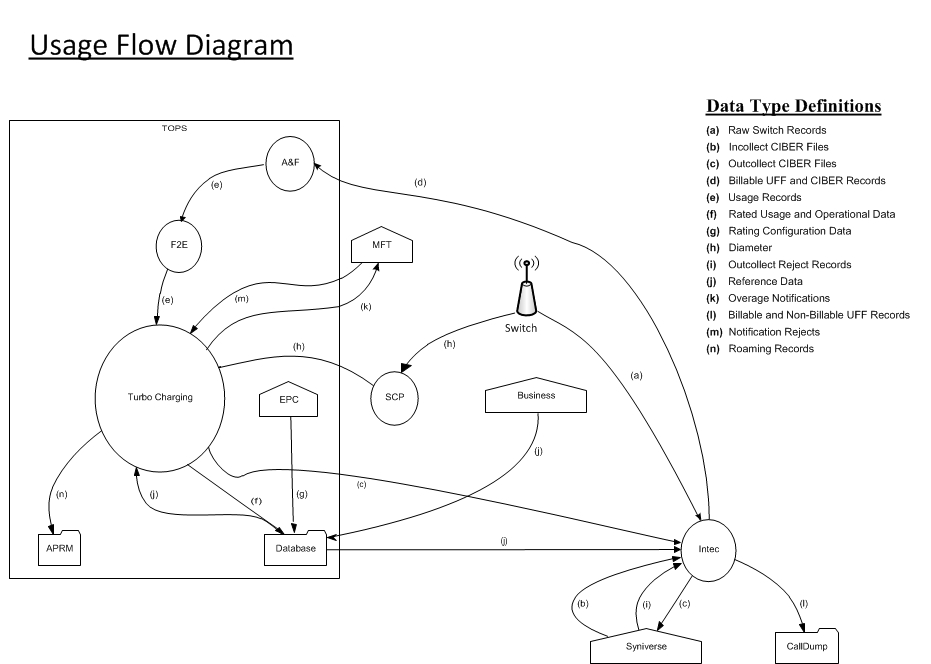
\includegraphics[width=20cm]{Pictures/usage_flow.jpg}
\end{landscape} 
\newpage
\begin{landscape}  
\subsection{Pre-Pay and Data Roaming}
\label{sec-2-5}

    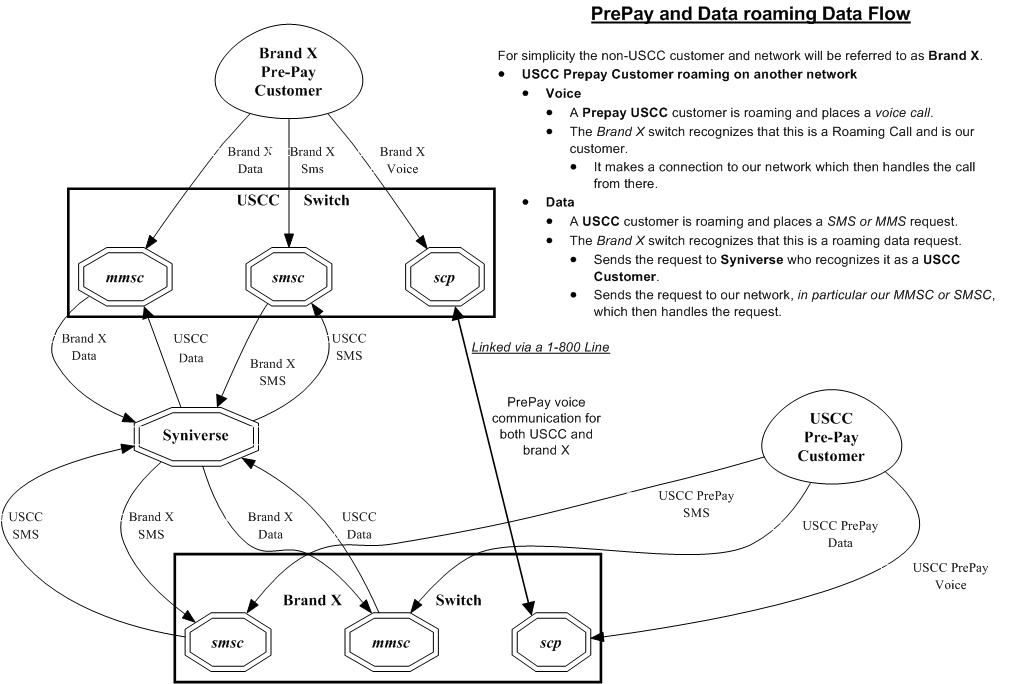
\includegraphics[width=23cm]{Pictures/roamingPrePay.png}
\end{landscape} 
\newpage
\section{TOPS Usage Processing Operations}
\label{sec-3}
\subsection{Acquisition and Formating (A\&F)}
\label{sec-3-1}

  \textbf{A\&F} is to the new system what \textbf{MAF and RBMS} was to the old. Since
  the majority of rules will be moved to \textbf{INTEC, A\&F's} primary
  function in the \textbf{post-TOPS} world will be to move the data from the
  \textbf{UFF} to the usage record\footnote{\textbf{CIBER} - InCollect processing is still handled by \textbf{A\&F} and \textbf{RBMS}
 }.  If an \textbf{A\&F} error does
  occur the record will be dumped into a file to be later processed by
  the \textbf{AEM} \emph{(Amdocs Error Manager)}.
  
\subsection{TurboCharging}
\label{sec-3-2}

  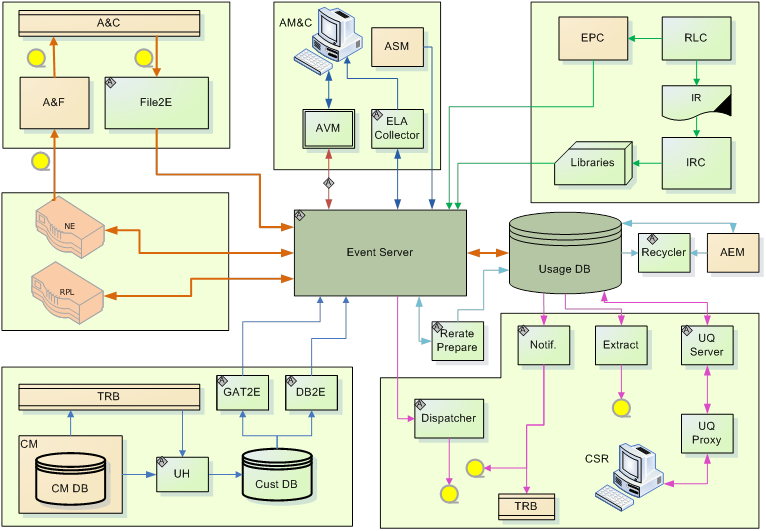
\includegraphics[width=17.5cm]{Pictures/TC.png}
  Though the overall architecture seems to be the same, with some name changes like \textbf{MAF} is now A\&F\footnote{Acquisitions and Formatting
 }, as \textbf{CARES} the major change has been the addition of the new real-time rater which \textbf{Amdocs} calls \textbf{Turbo Charging} that can handle both PRE and POST pay customers.\\
\begin{itemize}
\item All interaction is done through the network interface.
\item All tables are now in memory to improve performance.
\item We can re-rate continuously by running re-rating in daemon mode.
\item We can rate in other units beside minutes like \textbf{Content, Volume, Qos}.
\item Rating can be by step or tiered.
\item \textbf{Event flow:}
\begin{enumerate}
\item An event comes in to via a network element
\item Transforms data into a conical form which also includes the network element.
\item Gets Rated
\begin{itemize}
\item For \textbf{Pre-Pay} the HLR\footnote{Home Location Register
 }. is handled by the \textbf{SCP}
\end{itemize}
\item The response is sent back to the calling network element.
\end{enumerate}
\item \textbf{International Calls} are rated to the country not the individual city/town.
\item Find that in \textbf{LD\_COUNTRY\_RATES} table.
\item For \textbf{Pre-Pay} roaming customers still get a record which needs to go through \textbf{CIBER} process.
\item Major problem for \textbf{CCMI}. It was decided to remove it but the \textbf{LERG} does not give us the granularity that we might need.
\item For \textbf{Pre-Pay} \textbf{MMS} we will not charge each recipient only the sender.
\item We convert everything to the \textbf{Home SID time} for bill presentment.
\item Limiting or \emph{choking} usage can be handled by \textbf{Diameter} for real-time and \textbf{Turbo-Charging} for \textbf{Post-Pay}
\end{itemize}
\subsubsection{RLC (Rating Logic configurator)}
\label{sec-3-2-1}

\begin{itemize}
\item The \textbf{RLC} has a repository that keeps it rules as an \textbf{XML} string
     in a \emph{database column}.
\item Though they are stored as \textbf{XML} you can view them as \textbf{Product Catalog UI}.
\begin{itemize}
\item \textbf{Customer} defines set of attributes possibly having different values for different \textbf{customers/subscribers}.These attributes are further used in qualification criteria to define guiding to service functionality, and in event handlers to personalize pricing logic for specific customer/subscriber
\item \textbf{Performance Indicator} defines set of attributes (counters) to keep accumulated usage for some specific pricing item Its attributes are used and modified by the event handlers logic.
\item \textbf{Item Parameters} define a set of attributes that are the parameters of the Pricing Item Type Their values are set in the Product Catalog UI tool while creating a Pricing Item based on a given Pricing Item Type
\item \textbf{External record} defines a set of attributes associated with a specific extract record layout.
\item \textbf{Variables} define a set of attributes (variables) are used by handlers statements.
\end{itemize}
\item \textbf{PIT} \emph{Pricing Item Type}
\item We can define a number of different \textbf{Rating roles} and rating events.
\item Incoming calls are not dropped but instead are zero rated.
\end{itemize}
\begin{itemize}

\item Configuration Tools\\
\label{sec-3-2-1-1}%
The tool is a split screen application. On the left side contains
    all the rating schemes which are then dragged and dropped to
    create a tree structure on the right side.

\begin{itemize}
\item \textbf{RLC - Rating Logic configurator} \emph{Used to configure the rating engine}
\item Uses the \textbf{EPC} to create the rating logic, not the price
       plans. Once your finished with the configurator you the compile
       with the \textbf{ICC (Implementation Compiler configurator)} which
       then creates C++ code thats added to the rater.
\item \textbf{TCC (Turbo-Charging configurator)} - Used to configure the
       Turbo-Charging rater.
\item \textbf{Replenishment Manager} - Used for \textbf{Pre-Pay}.
\end{itemize}
\end{itemize} % ends low level
\subsection{Production Servers/EpsMonitors}
\label{sec-3-3}

\small
\begin{itemize}
\item \textbf{Batch1} - \textbf{kprl1batch.uscc.com (10.176.177.177)}
\begin{itemize}
\item \//pkgbl01\//inf\//aimsys\//prdwrk1\//eps\//monitors
\end{itemize}
\item \textbf{Batch2} - \textbf{kprl2batch.uscc.com (10.176.177.178)}
\begin{itemize}
\item \//pkgbl02\///inf\//aimsys\//prdwrk2\//eps\//monitors
\end{itemize}
\item \textbf{Batch3} - \textbf{kprl3batch.uscc.com (10.176.177.179)}
\begin{itemize}
\item \//pkgbl03\//inf\//aimsys\//prdwrk3\//eps\//monitors
\end{itemize}
\item \textbf{Batch4} – \textbf{kprl6batch.uscc.com (10.176.181.123)}
\item \textbf{Event1} – \textbf{kprl1event.uscc.com (10.176.181.116)}
\item \textbf{Event2} – \textbf{kprl2event.uscc.com (10.176.181.117)}
\item \textbf{Event3} – \textbf{kprl3event.uscc.com (10.176.181.118)}
\item \textbf{Event4} – \textbf{kprl4event.uscc.com (10.176.181.119)}
\item \textbf{Event5} – \textbf{kprl5event.uscc.com (10.176.181.120)}
\item \textbf{Event6} – \textbf{kprl6event.uscc.com (10.176.181.121)}
\item \textbf{APRM} - \textbf{kprl1batch.uscc.com (10.176.177.179)}
\begin{itemize}
\item \//inf\_nas\//apm1\//prod\//aprmoper\//eps\//monitors\textbackslash{}
\end{itemize}
\end{itemize}
\normalsize
\subsection{Event Servers}
\label{sec-3-4}

   There are multiple Event Servers which coresspond to bill cycle and run on the event servers.   
   Their status can be viewed using the following query on the \textbf{PRDAF} database. 
\begin{verbatim}
    SELECT * FROM ADJ3_JOBS_INST_CTRL WHERE JOB_NAME = 'ADJ1EVENTSRV';
\end{verbatim}
   From the output if the column \textbf{event status = Y} then that particular server is in use. 
   If your job requires an event server that is already in use you can change it to one that is not by using \textbf{SQL} below on the \textbf{PRDCUST} database logged in as \textbf{PRDOPRC}. 

   In this example we are setting the job rec to run using the \textbf{ES\_EOC1045} event server 

\begin{verbatim}
    Update OP_APP_DATA set data = 'ES_EOC1045'
           where JOB_REC = '{Your Job Rec}' and field_seq_num = 1 
           and table_NAME IN ('ADJ1EVENTSRV');
\end{verbatim}
\subsection{Rerate Servers}
\label{sec-3-5}

   There are three \textbf{Rerate Servers} they are:
\small
\begin{enumerate}
\item \textbf{RRP\_EOC1056}
\item \textbf{RRP\_EOC1068}
\item \textbf{RRP\_EOC1192}
\end{enumerate}
\normalsize
\subsection{OutCollect Operational Jobs (CIBER Processing)}
\label{sec-3-6}

  \textbf{CIBER} files are a collection of roaming records, these can be
  either a foreign carrier on our network or one of our customers
  on another network. More succinctly there are two
  types of roaming scenarios.
\begin{enumerate}
\item \textbf{OutCollects}\\ Non-USCC customers using our network, eventually
       the records created become part of the \textbf{OutCollect} process.
\item \textbf{InCollects}\\ USCC customers roaming on another carriers
       network. These records are sent to Syniverse which in turn
       sends them to us and become part of our \textbf{InCollect} process. All though InCollects come pre-rated they are still re-rated according to their plan.
\end{enumerate}

   The OutCollect process runs twice a day \textbf{1:00 a.m/p.m.}
\small
\begin{itemize}
\item \textbf{OUTCOL} \\ Extracts from the \textbf{APE1\_RATED\_EVENT} table and creates files for \textbf{MAS}.
\item \textbf{ADJ9MAS OUTCOL}\\ Creates files for \textbf{SPL1}.
\item \textbf{SPL1} - \emph{Daemon}\\ Processes files as it sees them and creates files for \textbf{RGD}.
\item \textbf{RGD} - \emph{Daemon}\\ Processes files as it sees them and creates files for \textbf{APP}.
\item \textbf{APP} - \emph{Daemon}\\ Processes files in RD after 12 hours of the last files processed. Output files for \textbf{Syniverse}.
\item \textbf{MF9FTDTAX}\\ Loads data into \textbf{MF9\_OUTCOL\_TAXES} table
\item \textbf{AR9OUTCLTAX}\\ End-day after \textbf{MF9FTDTAX}.
\end{itemize}
\normalsize
\subsubsection{OutCollect Files}
\label{sec-3-6-1}

   These are the file that are created by \textbf{TOPS} that will be sent to \textbf{Syniverse}.
\begin{itemize}
\item \textbf{aprout (OutCollect Directory)} \\
\end{itemize}
   \textbf{\//pkgbl02\//inf\//aimsys\//prdwrk2\//var\//usc\//projs\//apr\//interfaces\//output}
\subsubsection{Operational Tables}
\label{sec-3-6-2}
\begin{itemize}

\item \textbf{AC1\_CONTROL}\\
\label{sec-3-6-2-1}%
The Outbound Syniverse files
\begin{verbatim}
       select * from ac1_control
       where nxt_pgm_name = 'CBRRPT'
       and cur_pgm_name = 'APP'
      
       FILE_NAME
       ---------
       CIBER_CIBER_20130917090101_1312027_0001.dat
       CIBER_CIBER_20131012092425_1237215_0013.dat
       CIBER_CIBER_20130927090046_1027159_0012.dat
       ...
       CIBER_CIBER_20131011211952_1237215_0012.dat
\end{verbatim}

\item \textbf{MF1\_CIBER\_BATCH\_SEQ}\\
\label{sec-3-6-2-2}%
Contain the CIBER batch sequence numbers \emph{(See Database Section)}.
\end{itemize} % ends low level
\subsection{Overage Protection}
\label{sec-3-7}

   Overage notifications are detected on an event by event basis. As events are processed by \textbf{TC} and added to 
   the \textbf{APE1\_ACCUMULATORS} table a check is made against the \textbf{L9\_FIRST\_THRESHOLD/L9\_SECOND\_THRESHOLD} fields. If an overage is detected the ***FIELD*** CTN is added to file (segregated by unique \textbf{TC} file?) in the NTF directory. MFT then pulls these files and delivers to DMI for distribution. A note is added to the NOTIFICATION\_HUB.SMS\_NOTIFICATION table (ODS) indicating the message was sent by DMI.
\subsubsection{Overage process flow}
\label{sec-3-7-1}

   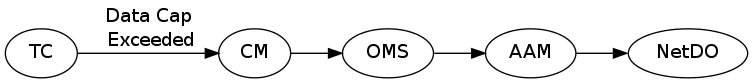
\includegraphics[width=15cm]{Pictures/overage.png}
\subsubsection{Output Location}
\label{sec-3-7-2}

\begin{verbatim}
   select notif_desc, file_path from CM9_NOTIFICATION_DEF
   where  FILE_PATH = '$ABP_APR_ROOT/interfaces/output/NTF'
   and FILE_ALIAS = 'SMSNTF'
\end{verbatim}
\footnotesize

\begin{center}
\begin{tabular}{ll}
\hline
 \textbf{NOTIF\_DESC}                     &  \textbf{FILE\_PATH}                     \\
\hline
 Overage cap notification on group level  &  \$ABP\_APR\_ROOT/interfaces/output/NTF  \\
 Disclaimer notification on group level   &  \$ABP\_APR\_ROOT/interfaces/output/NTF  \\
 Bucket notification on group level       &  \$ABP\_APR\_ROOT/interfaces/output/NTF  \\
\hline
\end{tabular}
\end{center}




\begin{center}
\begin{tabular}{l}
 \textbf{prdwrk1@kprl1batch:/pkgbl01/inf/aimsys/prdwrk1/var/usc/projs/apr/interfaces/output/NTF}  \\
\end{tabular}
\end{center}


\footnotesize
\subsubsection{Fields of Interest}
\label{sec-3-7-3}

    S - SMS, M - MMS, V - Voice, D - Data, L - LTE => L3\_CALL\_SOURCE
\subsection{Billing Process}
\label{sec-3-8}

  The billing process follows a map which is created by the job \textbf{ADJ3\_APR\_CycleBillRun\_Sh}. If it completes successfully it will create a billing map that will look something like the following:


  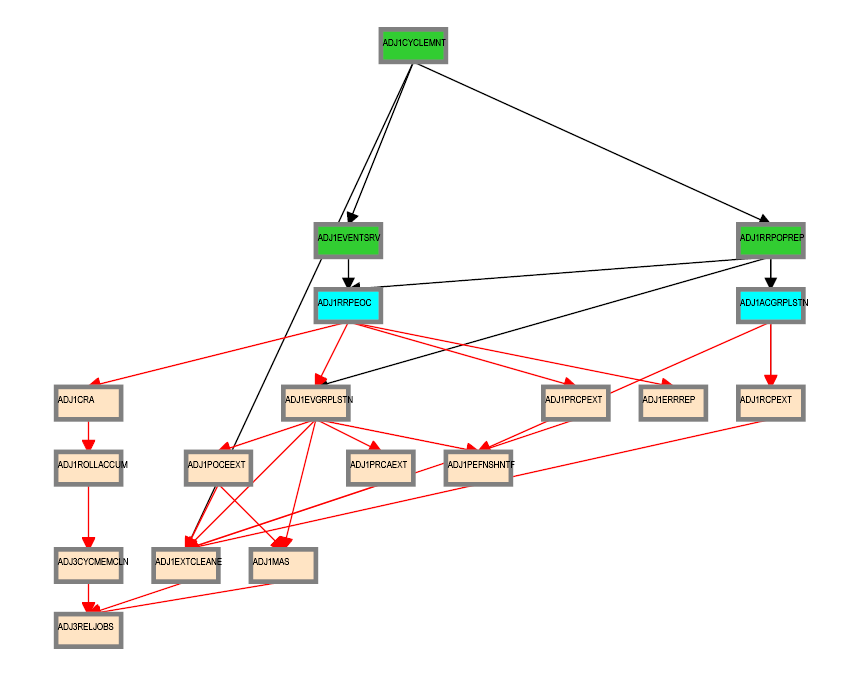
\includegraphics[width=15.5cm]{Pictures/billing_tc_map-27124108.png}
\subsection{Log File Location}
\label{sec-3-9}
\subsubsection{Batch 1}
\label{sec-3-9-1}

\begin{itemize}
\item cdlog - \//pkgbl01\//inf\//aimsys\//prdwrk1\//var\//usc\//log
\item A\&F | ssh prdwrk2@kpr02batch | MF1\_MD\_MD\_USC
\item F2E | ssh prdwrk4@kpr02batch | ADJ1\_File2E\_Daemon\_Shell\_Sh\_F2E
\end{itemize}
\subsection{Alias}
\label{sec-3-10}

\begin{itemize}
\item \textbf{cdlog} - cd to the logfile directory.
\item \textbf{cdswitch (Batch1 Only)} - cd to the switch directory.
\item \textbf{aprout} - cd to the \textbf{CIBER} out directories.
\end{itemize}
\subsection{Operational Terms and Definitions}
\label{sec-3-11}

\begin{itemize}
\item \textbf{Front-end Processes}
\begin{itemize}
\item \textbf{CRM:} Customer Relationship Manager
\begin{itemize}
\item \textbf{Smart Client Designer}
\item \textbf{ASCF Designer - Amdocs Smart Client Designer}
\item \textbf{APM - Amdocs Process manager}
\end{itemize}
\item \textbf{RIM:}  Retail Interaction Manager
\begin{itemize}
\item \textbf{POS:} Point of sale provided by \textbf{Microtelecom}
\item \textbf{Pricing Studio}
\item \textbf{ASM Amdocs Security Module}
\end{itemize}
\end{itemize}
\item \textbf{Provisioning}
\begin{itemize}
\item \textbf{AM or AAM - Activation Manager:} Provision Tool
\begin{itemize}
\item \textbf{APM:} The Gui front end to \textbf{AM}
\end{itemize}
\end{itemize}
\item \textbf{Usage Acquisition and Rating}
\begin{itemize}
\item \textbf{A\&F} Acquisition and formatting
\item \textbf{Turbo-Charging} Real-time rater
\begin{itemize}
\item \textbf{SCP} - Session Control Protocol
\end{itemize}
\item \textbf{MAF now called Acquisition and Formatting}
\item \textbf{AMC - Amdocs Monitoring and control}
\item \textbf{AEM - Amdocs Error Manager} \emph{replaces EMS}
\item \textbf{RLC} - Rating Logic Configurator
\end{itemize}
\item \textbf{Billing}
\begin{itemize}
\item \textbf{Billing Configurator}
\item \textbf{Invoicing Configurator}
\item \textbf{Replenishment Manager}
\item \textbf{Designer Studio} \emph{for bill layout}
\item \textbf{Pooling} - Everyone brings there services to be shared within
     everyone in the pool. Pooling is customization.
\item \textbf{Sharing} - A finite set of resources are set-up and everyone can
     use it.
\item \textbf{MRC - Monthly Recurring Charge}
\end{itemize}
\item \textbf{Integration sub-systems}
\begin{itemize}
\item \textbf{AIF - Amdocs Integration Framework}
\item \textbf{\index{ASM}ASM - Amdocs Security Manager}
\item \textbf{APM - Amdocs Process Manager}
\item \textbf{MMI - Multimedia Integrator}
\item \textbf{OM - Order Manager}
\item \textbf{OMS - Order Management System}
\end{itemize}
\end{itemize}
\newpage
\section{TC Oncall Daily Duties:}
\label{sec-4}
\subsection{Check the Monitors}
\label{sec-4-1}
\subsubsection{Batch Tab}
\label{sec-4-1-1}

\begin{itemize}
\item Open Remedy against Amdocs - Tier 2 Billing to restart the scripts when any of the Batch1, Batch2, Batch3, or APRM columns are missing indicating they are down.
\item Open Remedy against Amdocs - Tier 2 Billing to restart the script when any of these scripts are red indicating they are down.\\
\textbf{Batch 1 APPS}\\

\begin{center}
\begin{tabular}{lll}
\hline
 Aged\_reject\_to\_close\_prdcust  &  Up  &  Jul23  \\
 AnFReport                         &  Up  &  Jul23  \\
 BillingTasks                      &  Up  &  Jul26  \\
 cpni\_auto                        &  Up  &  Jul23  \\
 ovpDmiRejectsWA                   &  Up  &  Jul26  \\
 ovpMonitorAuto                    &  Up  &  Jul24  \\
\hline
\end{tabular}
\end{center}


    \textbf{Batch 2 APPS}\\

\begin{center}
\begin{tabular}{lll}
\hline
 af\_fixer                     &  Up  &  Jul27  \\
 auto\_error\_handle\_PRDUSG1  &  Up  &  Jul27  \\
 auto\_error\_handle\_PRDUSG2  &  Up  &  Jul27  \\
 auto\_error\_handle\_PRDUSG3  &  Up  &  Jul27  \\
 auto\_error\_handle\_PRDUSG4  &  Up  &  Jul27  \\
 large\_charge                 &  Up  &  Jul27  \\
 Log\_Monitoring               &  Up  &  14:19  \\
 pseudoCron                    &  Up  &  Jul27  \\
 pseudoCron1day                &  Up  &  Jul27  \\
\hline
\end{tabular}
\end{center}


    \textbf{Batch 2 Filesystem}\\

\begin{center}
\begin{tabular}{lllll}
\hline
 \textbf{Folder}  &  \textbf{Size}  &  \textbf{Used}  &  \textbf{Available}  &  \textbf{Used}  \\
\hline
 /var             &  1.9G           &  267M           &  1.6G                &  15\%           \\
 /tmp             &  5.7G           &  1.8G           &  3.6G                &  34\%           \\
 /af              &  9.4T           &  2.1T           &  7.4T                &  23\%           \\
 /JP\_FS          &  5.9T           &  2.8T           &  3.2T                &  47\%           \\
\hline
\end{tabular}
\end{center}


\end{itemize}
\subsubsection{Event Tab}
\label{sec-4-1-2}

\begin{itemize}
\item Open Remedy against Amdocs - Tier 2 Billing to restart the scripts when any of the Event1 through Event6 columns are missing indicating they are down.
\item Open Remedy against Amdocs - Infra Environments to investigate available space when any of the File system \% Used sections are red.
\end{itemize}
\subsubsection{AC1 Control Tab}
\label{sec-4-1-3}

\begin{itemize}
\item Open Remedy against Amdocs  for AF and stuck in IU or RD files when creation date and is less than current date.
\item Use the A\&F monitor report for <MM/DD/YYYY> and APRM monitor report for <MM/DD/YYYY> emails as supporting evidence, which run every hour.
\end{itemize}
\subsubsection{AEM Tab}
\label{sec-4-1-4}

\begin{itemize}
\item Ignore – monitor  was turn off due a conflict with prepaid event transactions.
\end{itemize}
\subsubsection{Other Tab}
\label{sec-4-1-5}

\begin{itemize}
\item Open Remedy against Amdocs - Tier 2 Billing to check on going rerating when rows are in red for more than one day.
\end{itemize}
\subsection{Check Overage Protection Monitor.}
\label{sec-4-2}

\begin{itemize}
\item Go to the MPS mailbox and look for the Overage Notification Count for <MM-DD-YYYY> email.\\
When received with counts similar to these there are no issues.
\end{itemize}
\begin{verbatim}
    Total Files: 42987
    Total Records: 154323
    75%: 84418
    100%: 69830
    Disclaimer: 60
    Balance: 15
\end{verbatim}
\begin{itemize}
\item When count are significantly low open a Sev 3 ticket against Amdocs.
\end{itemize}
\begin{verbatim}
    Total Files: 2607
    Total Records: 9458
    75%: 5365
    100%: 4092
    Disclaimer: 0
    Balance: 1
\end{verbatim}
\begin{itemize}
\item Open a Sev 2 ticket against Amdocs when Overage Notification Count FAILED for <MM-DD-YYYY>! is received.
\begin{itemize}
\item Call IS Support at 608-828-5812 to inform them of a Sev 2 or above ticket.
\item Escalate ticket in Remedy, call Amdocs T2.5 on call at 217-766-1979.
\item Email applicable teams the ticket number and description.
\end{itemize}
\end{itemize}
\begin{verbatim}
    To:  GSSUSCCTier25RA@amdocs.com
    Cc:  USCDLISOps-BillingandAROperations@uscellular.com; MPS@uscellular.com
\end{verbatim}
 
\subsection{Check .LOG file monitor.}
\label{sec-4-3}

\begin{itemize}
\item Go to the MPS mailbox and look for the Log Monitoring Count for <MM-DD-YYYY> ! email
\item When received with No LOG files where found for  <MM-DD-YYYY> there are no issues.
\item When received with ``Log files found for <MM-DD-YYYY> Total Log Files:  <XXXXXX> open a sev 3 Remedy ticket against Amdocs.
\begin{itemize}
\item Escalate ticket in Remedy, call Amdocs T2.5 on call at 217-766-1979.
\item Email applicable teams the ticket number and description.
\end{itemize}
\begin{verbatim}
 To:  GSSUSCCTier25RA@amdocs.com
      Cc:  USCDLISOps-BillingandAROperations@uscellular.com; MPS@uscellular.com
\end{verbatim}
\end{itemize}
\subsection{Check AC1\_CONTROL Fixer Status.}
\label{sec-4-4}

\begin{itemize}
\item Go to the MPS mailbox and look for the AC1\_CONTROL Fixer Status emails.  There are two.  One at \~{}12:04AM and on at \~{}4:03AM.
\item The output is similar to what is shown below.  The only action needed is when a Sid is removed other than \textbf{SIDS} 45696, 49697, and 49698.  When a Sid other than the aforementioned \textbf{SIDS} is removed open a Sev 4 Remedy against Inter-carrier Services, email the ticket number, description, and details to Zachary.Gutter@uscellular.com asking him to validate the Sid.
 
\begin{verbatim}
     Results for the AC1_CONTROL Fixer:
\end{verbatim}
 
\begin{verbatim}
     Fixed /pkgbl02/inf/aimsys/prdwrk2/var/usc/projs/up/physical/
           switch/DIRI/SDIRI_FCIBER_ID000069_T20150802185115.DAT 
     and replaced it with /pkgbl02/inf/aimsys/prdwrk2/var/usc/projs
           /up/physical/switch/DIRI/SDIRI_FCIBER_ID000069_T20150802185199
\end{verbatim}

\begin{verbatim}
     Sid:  was removed
\end{verbatim}
 
\begin{verbatim}
     There were 0 CIBER AF files with wr_rec_quantity of 2
\end{verbatim}
 
\begin{verbatim}
     There were 0 out of sequence CIBER files
\end{verbatim}
 
\begin{verbatim}
     There were 0 OutColllects files stuck IU and set to RD
\end{verbatim}
 
\begin{verbatim}
     There were 0 File2E stuck IU/AF files and set to RD
\end{verbatim}
 
\begin{verbatim}
     There were 0 Files stuck FR files and set to RD
\end{verbatim}
 
\begin{verbatim}
     There were 21 ORG records updated at prdusg1c.ape1_subscriber_rerate
     from num_of_rerate_tries=3 to 1
\end{verbatim}
 
\begin{verbatim}
     There were 14 ORG records updated at prdusg2c.ape1_subscriber_rerate 
     from num_of_rerate_tries=3 to 1
\end{verbatim}
 
\begin{verbatim}
     There were 28 ORG records updated at prdusg3c.ape1_subscriber_rerate 
     from num_of_rerate_tries=3 to 1
\end{verbatim}
 
\begin{verbatim}
     There were 28 ORG records updated at prdusg4c.ape1_subscriber_rerate 
     from num_of_rerate_tries=3 to 1
\end{verbatim}
\end{itemize}
\subsection{Check Large Charge monitor.}
\label{sec-4-5}

\begin{itemize}
\item Go to the MPS mailbox and look for the Large Charge email.
\item When the subject line is other than Large Charge Not Detected - No Action Required open a sev 3 Remedy against Amdocs.
\begin{itemize}
\item Escalate ticket in Remedy, call Amdocs T2.5 on call at 217-766-1979.
\item Email applicable teams the ticket number and description.
\end{itemize}
\begin{verbatim}
 To:  GSSUSCCTier25RA@amdocs.com
      Cc:  USCDLISOps-BillingandAROperations@uscellular.com; MPS@uscellular.com
\end{verbatim}
\end{itemize}
\subsection{Check out of sequence CIBER records monitor.}
\label{sec-4-6}

\begin{itemize}
\item Go to the MPS mailbox and look for the out of sequence CIBER records email.
\item When the subject line is other than No out of sequence CIBER records for <YYYYMMDD> open a sev 4 Remedy against Amdocs.
\begin{itemize}
\item Email applicable teams the ticket number and description.
\end{itemize}
\end{itemize}
\begin{verbatim}
    To:  GSSUSCCTier25RA@amdocs.com
    Cc:  USCDLISOps-BillingandAROperations@uscellular.com; MPS@uscellular.com
\end{verbatim}
\subsection{When Notified Nonfictions.}
\label{sec-4-7}

\begin{itemize}
\item kpr01ebiap maintenance.
\begin{itemize}
\item Login to the EBI server with your LAN ID and password.
\item Check if AEM and KPI scripts are running.
\end{itemize}
\end{itemize}
\begin{verbatim}
    [md1dsmi1@kpr01ebiap eps]$ ps -ef | grep perl | grep md1dsmi1 | grep -v grep
    md1dsmi1   16566       1  0 Jul30 ?        00:00:00 perl ./aem_purge_trending_split.pl 1 0
    md1dsmi1 2345044       1  0 Jul28 ?        00:00:00 perl ./aem_error_trending_auto.pl
    md1dsmi1 2345048       1  0 Jul28 ?        00:00:00 perl ./aem_purge_trending_auto.pl
    md1dsmi1 2345050       1  0 Jul28 ?        00:00:00 perl ./em1_errors_trending_auto.pl
    md1dsmi1 2345052       1  0 Jul28 ?        00:00:00 perl ./em1_errors_write_off_auto.pl
    md1dsmi1 2345053       1  0 Jul28 ?        00:00:00 perl ./remedy_reports_auto.pl
    md1dsmi1 2345054       1  0 Jul28 ?        00:00:43 perl ./tc_kpi_auto.pl 2 2 1 1
    md1dsmi1 2345055       1  0 Jul28 ?        00:00:02 perl ./tc_kpi_datain_auto.pl 2 2 1 1
\end{verbatim}
\begin{itemize}
\item Check if Business Report scripts are running.
\end{itemize}
\begin{verbatim}
    [md1dsmi1@kpr01ebiap eps]$ ps -ef | grep MainLoop | grep -v grep
    md1dsmi1 2188567       1  0 Jul28 ?        00:00:00 HS1H MainLoop - next: 
    md1dsmi1 2188568       1  0 Jul28 ?        00:00:00 CancelLineIL MainLoop - next:
    md1dsmi1 2188569       1  0 Jul28 ?        00:00:00 MADISON MainLoop - next: 
    md1dsmi1 2188570       1  0 Jul28 ?        00:00:00 CancelLineWI MainLoop - next:
    md1dsmi1 2188571       1  0 Jul28 ?        00:00:00 daily_counts MainLoop - next:
\end{verbatim}
\subsection{Restart AEM and KPI scripts.}
\label{sec-4-8}

\begin{itemize}
\item Login to the EBI server with your LAN ID and password.
\item cd to /home/common/eps/das
\item Run from the command line nohup ./StartAllErrorAndKPI.sh \&
\end{itemize}
 
\subsection{Restart Business Report scripts.}
\label{sec-4-9}

\begin{itemize}
\item Login to the EBI server with your LAN ID and password.
\item cd to /home/common/eps/reports
\item Run from the command line nohup ./StartAllReportCron.sh \&
\end{itemize}
 
   Note all scripts use Dave Smith's LAN ID password and when the failure is due to the password being expired please notify him immediately and if he is out of the office wait until he returns to the office to reset his password and update the scripts.

\newpage
\section{Voice Overview}
\label{sec-5}

\normalsize
  One major undertaking in the transition to \textbf{TOPS} is moving most of
  the voice mediation to the \textbf{INTEC} platform. To help facilitate this
  move, the current rules system \textbf{(RBMS)} was studied and
  documented. The following provides a brief overview of the processes
  used. 
\subsection{Call Types}
\label{sec-5-1}

\small
\begin{enumerate}
\item \textbf{M-M} - Mobile to Mobile
\item \textbf{M-L} - Mobile to Land Line
\item \textbf{L-M} - Land Line to Mobile
\item \textbf{L-L} - Land Line to Land Line
\end{enumerate}
\normalsize
  The call records can come in four possible states. 
\small
\begin{enumerate}
\item Mobile Terminating (Incoming)
\item Mobile Originating (Outgoing)
\item \textbf{NTI ONLY}
\begin{itemize}
\item \textbf{Both} \\ \textbf{(NTI Mobile to Mobile)} in which for every voice event, two records
       are created, a \textbf{Mobile Originated} and \textbf{Mobile Terminated} record.
       For \textbf{APLX} this is taken care of automatically. In the case of an
       \textbf{NTI} switch, depending on the call scenario, it is up to the
       mediation platform to create one if needed.
\item \textbf{Neither} \\ (per example \textbf{L-L} )
\end{itemize}
\end{enumerate}
\normalsize

\begin{landscape}  
\subsection{Incoming}
\label{sec-5-2}

   An \textbf{Incoming} call is a \emph{mobile terminated} call where one of our customers receives a call from some caller to a \textbf{USCC} switch.\\
   \textbf{The diagram below shows the data flow for an incoming call:}\\ \\
   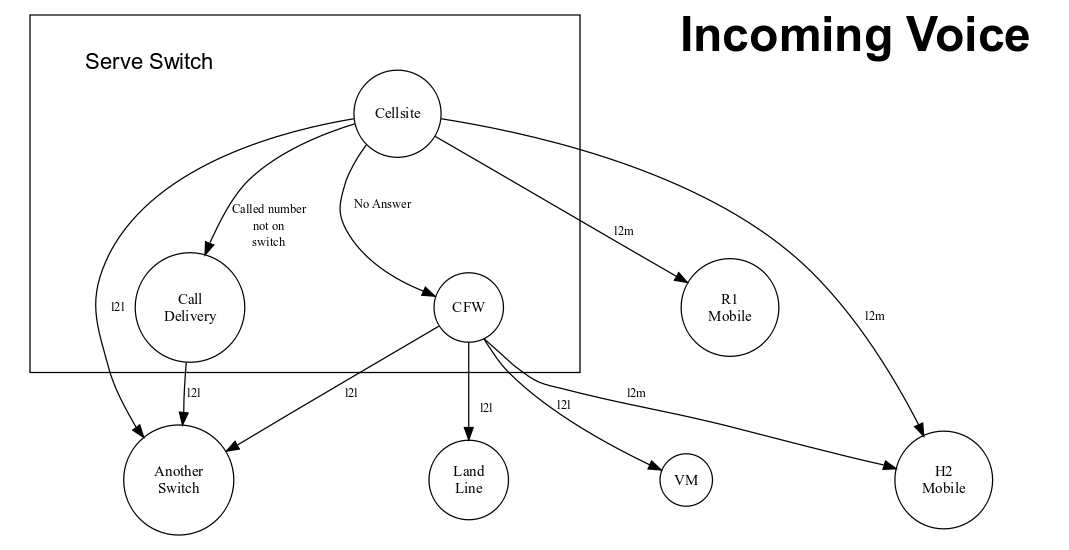
\includegraphics[width=20cm]{Pictures/incoming.png}

\end{landscape} 
\newpage
\begin{landscape}  
\subsection{Outgoing}
\label{sec-5-3}

   An \textbf{outgoing} call is a \emph{mobile originating} call from a \textbf{USCC}
   customer in which the following can occur. \\
   \textbf{The diagram below shows the data flow for an outgoing call:} \\ \\


    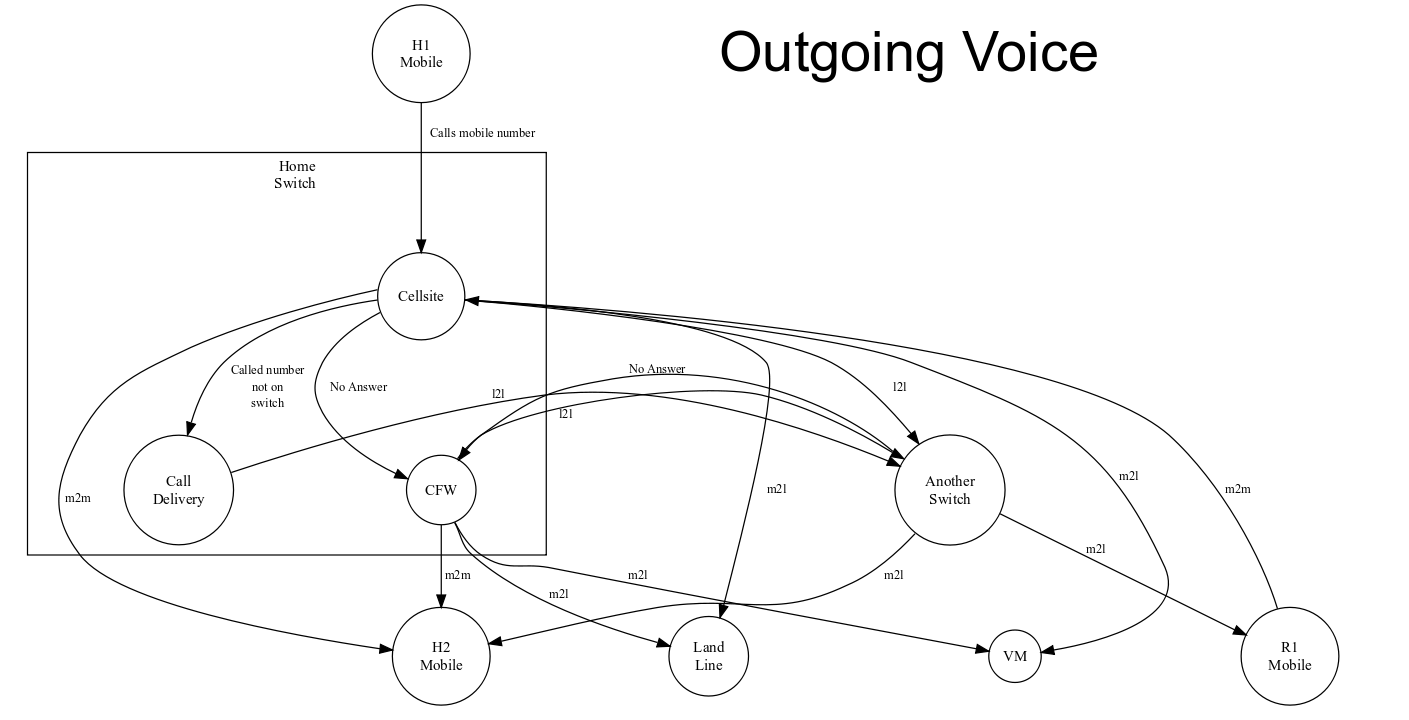
\includegraphics[width=23cm]{Pictures/outgoing.png}

\end{landscape} 
\newpage
\section{CIBER File Format}
\label{sec-6}
\subsection{Ciber Record Types}
\label{sec-6-1}

   The \textbf{Ciber} standard defines the following record Types:
\begin{itemize}
\item \textbf{01} Header
\item \textbf{22} Voice (main Record type)
\item \textbf{32} Data \emph{Need more info}
\item \textbf{52} One time charge
\item \textbf{98} Trailer
\end{itemize}
\subsection{CIBER 01 Record}
\label{sec-6-2}

\footnotesize
\begin{longtable}{lrr}

\hline
 \textbf{Field}                  &  \textbf{Position}  &  \textbf{Description} \\
\hline
\endhead
\hline\multicolumn{3}{r}{Continued on next page}\
\endfoot
\endlastfoot
 Record Type                     &                1-2  &                        \\
 Batch Creation Date             &                3-8  &                        \\
 Batch Sequence Number           &               9-11  &                        \\
 Sending Carrier SID/BID         &              12-16  &                        \\
 Receiving Carrier SID/BID       &              17-21  &                        \\
 CIBER Record Release Number     &              22-23  &                        \\
 Original/Return Indicator       &              24-24  &                        \\
 Currency Type                   &              25-26  &                        \\
 Settlement Period               &              27-32  &                        \\
 Clearinghouse ID                &              33-33  &                        \\
 CIBER Batch Reject Reason Code  &              34-35  &                        \\
 Batch Contents                  &              36-36  &                        \\
 Local Carrier Reserved          &              37-56  &                        \\
 System Reserved Filler          &             57-200  &                        \\
\hline
\end{longtable}

\normalsize
\subsection{CIBER 22 Record}
\label{sec-6-3}

\footnotesize
\begin{longtable}{lrl}

\hline
 \textbf{FIELD NAME}                       &  \textbf{POSITION}  &  \textbf{Description} \\
\hline
\endhead
\hline\multicolumn{3}{r}{Continued on next page}\
\endfoot
\endlastfoot
 Record Type                               &                1-2  &                        \\
 Return Code                               &                3-3  &                        \\
 CIBER Record Return Reason Code           &                4-5  &                        \\
 Invalid Field Identifier                  &                6-8  &                        \\
 Home Carrier SID/BID                      &               9-13  &                        \\
 MSID Indicator                            &              14-14  &                        \\
 \textbf{MSID}                             &              15-29  &                        \\
 MSISDN/MDN Length                         &              30-31  &                        \\
 \textbf{MSISDN/MDN}                       &              32-46  &                        \\
 \textbf{ESN/UIMID/IMEI/MEID Indicator}    &              47-47  &  0 = NA                \\
                                           &                     &  1 = ESN               \\
                                           &                     &  2 = IMEI              \\
                                           &                     &  3 = MEID              \\
                                           &                     &  4 = pESN              \\
 \textbf{ESN/UIMID/IMEI/MEID}              &              48-66  &                        \\
 \textbf{Serving Carrier SID/BID}          &              67-71  &                        \\
 \textbf{Total Charges and Taxes}          &              72-81  &                        \\
 System Reserved Filler                    &              82-82  &                        \\
 \textbf{Total State/Province Taxes}       &              83-92  &                        \\
 System Reserved Filler                    &              93-93  &                        \\
 \textbf{Total Local/Other Taxes}          &             94-103  &                        \\
 System Reserved Filler                    &            104-104  &                        \\
 \textbf{Call Date}                        &            105-110  &                        \\
 \textbf{Call Direction}                   &            111-111  &                        \\
 Call Completion Indicator                 &            112-112  &                        \\
 Call Termination Indicator                &            113-113  &                        \\
 Caller ID Length                          &            114-115  &                        \\
 Caller ID                                 &            116-130  &                        \\
 Called Number Length                      &            131-132  &                        \\
 \textbf{Called Number Digits}             &            133-147  &                        \\
 Location Routing Number Length Indicator  &            148-149  &                        \\
 Location Routing Number                   &            150-164  &                        \\
 TLDN Length                               &            165-166  &                        \\
 TLDN                                      &            167-181  &                        \\
 Currency Type                             &            182-183  &                        \\
 System Reserved Filler                    &            184-185  &                        \\
 Original Batch Sequence Number            &            186-188  &                        \\
 Initial Cell Site                         &            189-199  &                        \\
 Time Zone Indicator                       &            200-201  &                        \\
 Daylight Savings Indicator                &            202-202  &                        \\
 Message Accounting Digits                 &            203-212  &                        \\
 Air Connect Time                          &            213-218  &                        \\
 Air Chargeable Time                       &            219-224  &                        \\
 Air Elapsed Time                          &            225-230  &                        \\
 Air Rate Period                           &            231-232  &                        \\
 Air Multi-Rate Period                     &            233-233  &                        \\
 \textbf{Air Charge}                       &            234-243  &                        \\
 System Reserved Filler                    &            244-244  &                        \\
 Other Charge No. 1 Indicator              &            245-246  &                        \\
 \textbf{Other Charge No. 1}               &            247-256  &                        \\
 System Reserved Filler                    &            257-257  &                        \\
 System Reserved Filler                    &            258-270  &                        \\
 Printed Call                              &            271-285  &                        \\
 Fraud Indicator                           &            286-287  &                        \\
 Fraud Sub-Indicator                       &            288-288  &                        \\
 \textbf{Special Features Used}            &            289-293  &                        \\
 \textbf{Called Place}                     &            294-303  &                        \\
 \textbf{Called State/Province}            &            304-305  &                        \\
 \textbf{Called Country}                   &            306-308  &                        \\
 \textbf{Serving Place}                    &            309-318  &                        \\
 \textbf{Serving State/Province}           &            319-320  &                        \\
 \textbf{Serving Country}                  &            321-323  &                        \\
 Toll Connect Time                         &            324-329  &                        \\
 Toll Chargeable Time                      &            330-335  &                        \\
 Toll Elapsed Time                         &            336-341  &                        \\
 Toll Tariff Descriptor                    &            342-343  &                        \\
 Toll Rate Period                          &            344-345  &                        \\
 Toll Multi-Rate Period                    &            346-346  &                        \\
 Toll Rate Class                           &            347-347  &                        \\
 Toll Rating Point Length Indicator        &            348-349  &                        \\
 Toll Rating Point                         &            350-359  &                        \\
 \textbf{Toll Charge}                      &            360-369  &                        \\
 System Reserved Filler                    &            370-370  &                        \\
 \textbf{Toll State/Province Taxes}        &            371-380  &                        \\
 System Reserved Filler                    &            381-381  &                        \\
 \textbf{Toll Local Taxes}                 &            382-391  &                        \\
 System Reserved Filler                    &            392-392  &                        \\
 Toll Network Carrier ID                   &            393-397  &                        \\
 Local Carrier Reserved                    &            398-472  &                        \\
 System Reserved Filler                    &            473-547  &                        \\
\hline
\end{longtable}


\normalsize
\subsection{CIBER 32 Record}
\label{sec-6-4}

\footnotesize
\begin{longtable}{lrr}

\hline
 \textbf{Field}                            &  \textbf{Position}  &  \textbf{Description} \\
\hline
\endhead
\hline\multicolumn{3}{r}{Continued on next page}\
\endfoot
\endlastfoot
 Record Type                               &                1-2  &                        \\
 Return Code                               &                3-3  &                        \\
 CIBER Record Return Reason Code           &                4-5  &                        \\
 Invalid Field Identifier                  &                6-8  &                        \\
 Home Carrier SID/BID                      &               9-13  &                        \\
 MSID Indicator                            &              14-14  &                        \\
 MSID                                      &              15-29  &                        \\
 MSISDN/MDN Length                         &              30-31  &                        \\
 MSISDN/MDN                                &              32-46  &                        \\
 ESN/UIMID/IMEI/MEID Indicator             &              47-47  &                        \\
 ESN/UIMID/IMEI/MEID                       &              48-66  &                        \\
 Serving Carrier SID/BID                   &              67-71  &                        \\
 Total Charges and Taxes                   &              72-81  &                        \\
 System Reserved Filler                    &              82-82  &                        \\
 Total State/Province Taxes                &              83-92  &                        \\
 System Reserved Filler                    &              93-93  &                        \\
 Total Local Taxes                         &             94-103  &                        \\
 System Reserved Filler                    &            104-104  &                        \\
 Call Date                                 &            105-110  &                        \\
 Call Direction                            &            111-111  &                        \\
 Call Completion Indicator                 &            112-112  &                        \\
 Call Termination Indicator                &            113-113  &                        \\
 Caller ID Length                          &            114-115  &                        \\
 Caller ID                                 &            116-130  &                        \\
 Called Number Length                      &            131-132  &                        \\
 Called Number Digits                      &            133-147  &                        \\
 Location Routing Number Length Indicator  &            148-149  &                        \\
 Location Routing Number                   &            150-164  &                        \\
 TLDN Length                               &            165-166  &                        \\
 TLDN                                      &            167-181  &                        \\
 Currency Type                             &            182-183  &                        \\
 System Reserved Filler                    &            184-185  &                        \\
 Original Batch Sequence Number            &            186-188  &                        \\
 Initial Cell Site                         &            189-199  &                        \\
 Time Zone Indicator                       &            200-201  &                        \\
 Daylight Savings Indicator                &            202-202  &                        \\
 Message Accounting Digits                 &            203-212  &                        \\
 Charge No. 1 Indicator                    &            213-214  &                        \\
 Charge No. 1 Connect Time                 &            215-220  &                        \\
 Charge No. 1 Chargeable Time              &            221-226  &                        \\
 Charge No. 1 Elapsed Time                 &            227-232  &                        \\
 Charge No. 1 Rate Period                  &            233-234  &                        \\
 Charge No. 1 Multi-Rate Period            &            235-235  &                        \\
 Charge No. 1 Tax/Surcharge Indicator      &            236-236  &                        \\
 Charge No. 1                              &            237-246  &                        \\
 System Reserved Filler                    &            247-247  &                        \\
 Charge No. 2 Indicator                    &            248-249  &                        \\
 Charge No. 2 Connect Time                 &            250-255  &                        \\
 Charge No. 2 Chargeable Time              &            256-261  &                        \\
 Charge No. 2 Elapsed TIme                 &            262-267  &                        \\
 Charge No. 2 Rate Period                  &            268-269  &                        \\
 Charge No. 2 Multi-Rate Period            &            270-270  &                        \\
 Charge No. 2 Tax/Surcharge Indicator      &            271-271  &                        \\
 Charge No. 2                              &            272-281  &                        \\
 System Reserved Filler                    &            282-282  &                        \\
 Charge No. 3 Indicator                    &            283-284  &                        \\
 Charge No. 3 Connect Time                 &            285-290  &                        \\
 Charge No. 3 Chargeable Time              &            291-296  &                        \\
 Charge No. 3 Elapsed Time                 &            297-302  &                        \\
 Charge No. 3 Rate Period                  &            303-304  &                        \\
 Charge No. 3 Multi-Rate Period            &            305-305  &                        \\
 Charge No. 3 Tax/Surcharge Indicator      &            306-306  &                        \\
 Charge No. 3                              &            307-316  &                        \\
 System Reserved Filler                    &            317-317  &                        \\
 Charge No. 4 Indicator                    &            318-319  &                        \\
 Charge No. 4 Connect Time                 &            320-325  &                        \\
 Charge No. 4 Chargeable Time              &            326-331  &                        \\
 Charge No. 4 Elapsed Time                 &            332-337  &                        \\
 Charge No. 4 Rate Period                  &            338-339  &                        \\
 Charge No. 4 Multi-Rate Period            &            340-340  &                        \\
 Charge No. 4 Tax/Surcharge Indicator      &            341-341  &                        \\
 Charge No. 4                              &            342-351  &                        \\
 System Reserved Filler                    &            352-352  &                        \\
 Blank Fill Serving Place                  &            353-362  &                        \\
 Serving State/Province                    &            363-364  &                        \\
 Serving Country                           &            365-367  &                        \\
 Special Features Used                     &            368-372  &                        \\
 Other Charge No. 1 Indicator              &            373-374  &                        \\
 Other Charge No. 1                        &            375-384  &                        \\
 System Reserved Filler                    &            385-385  &                        \\
 System Reserved Filler                    &            386-398  &                        \\
 Printed Call                              &            399-413  &                        \\
 Fraud Indicator                           &            414-415  &                        \\
 Fraud Sub-Indicator                       &            416-416  &                        \\
 Features Used After Handoff Indicator     &            417-417  &                        \\
 Local Carrier Reserved                    &            418-492  &                        \\
 System Reserved Filler                    &            493-567  &                        \\
\hline
\end{longtable}

\normalsize
\subsection{CIBER 52 Record}
\label{sec-6-5}

\footnotesize
\begin{longtable}{lrr}

\hline
 \textbf{FIELD}                       &  \textbf{POSITION}  &  \textbf{Description} \\
\hline
\endhead
\hline\multicolumn{3}{r}{Continued on next page}\
\endfoot
\endlastfoot
 Return Code                          &                3-3  &                        \\
 CIBER Record Return Reason Code      &                4-5  &                        \\
 Invalid Field Identifier             &                6-8  &                        \\
 Home Carrier SID/BID                 &               9-13  &                        \\
 MSID Indicator                       &              14-14  &                        \\
 \textbf{MSID}                        &              15-29  &                        \\
 MSISDN/MDN Length                    &              30-31  &                        \\
 MSISDN/MDN                           &              32-46  &                        \\
 ESN/UIMID/IMEI/MEID Indicator        &              47-47  &                        \\
 ESN/UIMID/IMEI/MEID                  &              48-66  &                        \\
 Serving Carrier SID/BID              &              67-71  &                        \\
 \textbf{Total Charges and Taxes}     &              72-81  &                        \\
 System Reserved Filler               &              82-82  &                        \\
 \textbf{Total State/Province Taxes}  &              83-92  &                        \\
 System Reserved Filler               &              93-93  &                        \\
 \textbf{Total Local Taxes}           &             94-103  &                        \\
 System Reserved Filler               &            104-104  &                        \\
 \textbf{OCC Charge/Start Date}       &            105-110  &                        \\
 Connect Time                         &            111-116  &                        \\
 OCC End Date                         &            117-122  &                        \\
 OCC Interval Indicator               &            124-133  &                        \\
 \textbf{OCC Charge}                  &            134-134  &                        \\
 System Reserved Filler               &            135-159  &                        \\
 OCC Description Currency Type        &            160-161  &                        \\
 System Reserved Filler               &            123-123  &                        \\
 Original Batch Sequence Number       &            164-166  &                        \\
 Initial Cell Site                    &            167-177  &                        \\
 Time Zone Indicator                  &            178-179  &                        \\
 Daylight Savings Indicator           &            180-180  &                        \\
 Message Accounting Digits            &            181-190  &                        \\
 Record Use Indicator                 &            191-191  &                        \\
 Serving Place                        &            192-201  &                        \\
 Serving State/Province               &            202-203  &                        \\
 Serving Country                      &            204-206  &                        \\
 Other Charge No. 1 Indicator         &            207-208  &                        \\
 Other Charge No. 1                   &            209-218  &                        \\
 System Reserved Filler               &            219-219  &                        \\
 System Reserved Filler               &            220-232  &                        \\
 Fraud Indicator                      &            233-234  &                        \\
 Fraud Sub-Indicator                  &            235-235  &                        \\
 Record Create Date                   &            236-241  &                        \\
 System Reserved Filler               &            220-232  &                        \\
 Fraud Indicator                      &            233-234  &                        \\
 Fraud Sub-Indicator                  &            235-235  &                        \\
 Record Create Date                   &            236-241  &                        \\
\hline
\end{longtable}

\normalsize
\subsection{CIBER 98 Record}
\label{sec-6-6}

\footnotesize
\begin{longtable}{lrr}

\hline
 \textbf{FIELD}                            &  \textbf{POSITION}  &  \textbf{Description} \\
\hline
\endhead
\hline\multicolumn{3}{r}{Continued on next page}\
\endfoot
\endlastfoot
 Record Type                               &                1-2  &                        \\
 Batch Creation Date                       &                3-8  &                        \\
 Batch Sequence Number                     &               9-11  &                        \\
 Sending Carrier SID/BID                   &              12-16  &                        \\
 Receiving Carrier SID/BID                 &              17-21  &                        \\
 \textbf{Total Number Records in Batch}    &              22-25  &                        \\
 \textbf{Batch Total Charges \& Taxes}     &              26-37  &                        \\
 Settlement Period                         &              38-43  &                        \\
 Clearinghouse ID                          &              44-44  &                        \\
 System Reserved Filler                    &              45-49  &                        \\
 Original Total Number of Records          &              50-53  &                        \\
 \textbf{Original Total Charges \& Taxes}  &              54-65  &                        \\
 System Reserved Filler                    &              66-73  &                        \\
 Currency Type                             &              74-75  &                        \\
 Local Carrier Reserved                    &              76-95  &                        \\
 System Reserved Filler                    &             96-200  &                        \\
\hline
\end{longtable}

\normalsize
\subsection{US Territories}
\label{sec-6-7}

   These calls are identified as international but are charged domestic rates.
\footnotesize

\begin{center}
\begin{tabular}{rrll}
\hline
 Country Code  &  Area Code  &  ISO Country Code  &  Description                   \\
\hline
            1  &        340  &  VIR               &  United States Virgin Islands  \\
            1  &        670  &  MNP               &  Northern Mariana Islands      \\
            1  &        671  &  GUM               &  Guam                          \\
            1  &        684  &  ASM               &  American Samoa                \\
            1  &    787/939  &  PRI               &  Puerto Rico                   \\
\hline
\end{tabular}
\end{center}


\normalsize
\\
\subsection{Interfaces}
\label{sec-6-8}
\subsubsection{Roamex/Fraudex}
\label{sec-6-8-1}

    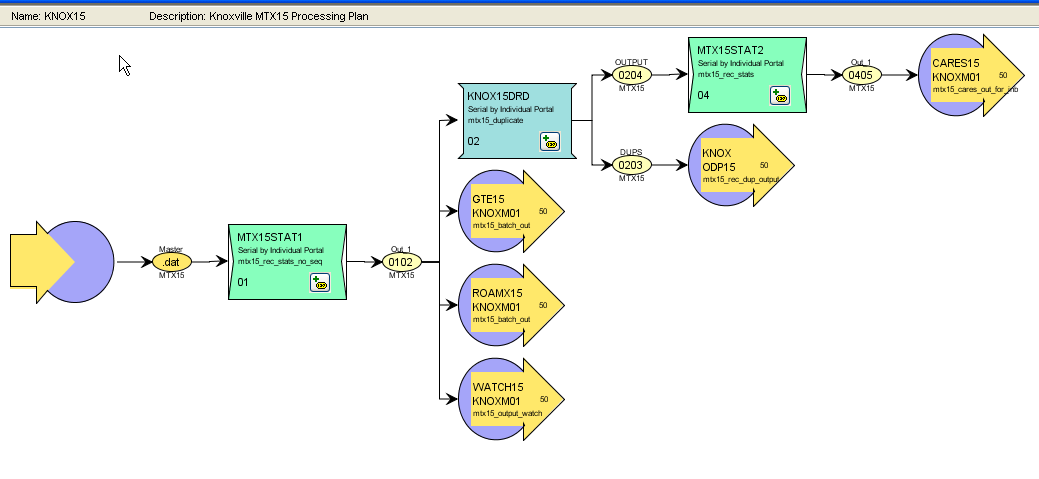
\includegraphics[width=13cm]{Pictures/NDC.png}
\begin{itemize}
\item \textbf{Business Process -} Mediation
\item \textbf{Type -} Batch
\item \textbf{Category -} Batch Redesign
\item \textbf{Service -}   On all \textbf{Nortel} switches switch records are
           copied to \textbf{mad1rom1}. Then through out the day \textbf{Syniverse}
           comes in and finds all the roaming records and runs it
           against there \textbf{Fraudx} application to find evidence of
           fraud.
\item \textbf{Thoughts and other random musings} \\ For the most part
           the process is a black box and everything is handled by
           \textbf{Syniverse}. The file that is sent is raw switch data and at this time
           only \textbf{NTI (Nortel)} is supported. For all NDC processes the source,
           compilation and processing occur on the NDC machines where
           the base language is C.
\item \textbf{Questions}
\begin{itemize}
\item $\Box$ What are the names of the NDC machines.
\item $\Box$ Where is the source code kept.
\end{itemize}
\item \textbf{Contacts}
\begin{itemize}
\item Kyle Matte
\item Roberto Amezcua
\end{itemize}
\end{itemize}
\subsubsection{OutCollects}
\label{sec-6-8-2}

    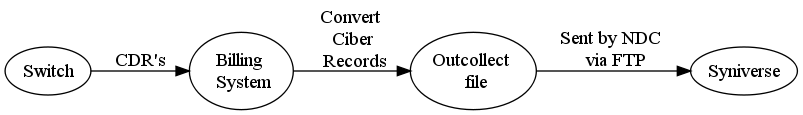
\includegraphics[width=13cm]{Pictures/outcoll.png}
\begin{itemize}
\item \textbf{Business Process -} Mediation
\item \textbf{Type -} Batch
\item \textbf{Category -} Batch Redesign
\item \textbf{Service -}  Send OutCollect data to \textbf{Syniverse}.
\item \textbf{Process Flow}
\begin{enumerate}
\item Switch records are passed through the billing system and any
        record that does not belong to a customer gets placed into a file.
\item Twice a day the \emph{Ciber\_Create} job is run which takes these
        files and converts them to CIBER records.
\item Five times a day \textbf{NDC} starts a job which sends these files to
        \textbf{Syniverse}.
\item It also when it looks for CIBER files coming back from
        \textbf{Syniverse} of our customers who are roaming on other networks.
\end{enumerate}
\item \textbf{Thoughts and other random musings} \\ A pretty simple batch
     interface it is here where we can use the new batch standards to
     make sure the transfer is complete.
\item \textbf{Contacts}
\begin{itemize}
\item Kyle Matte
\item Roberto Amezcua
\end{itemize}
\end{itemize}
\subsection{CIBERNET - Specification/Reference}
\label{sec-6-9}

   \href{https://www.one1clear.net/mxp/Login.asp}{https://www.one1clear.net/mxp/Login.asp}
\begin{itemize}
\item Mobile-X Code: USA-MPS-0001
\item Login: Skeup/SyFAGh
\end{itemize}
\begin{verbatim}
     <\\chil-data1\Share\Common\TOPS\outcollects>
\end{verbatim}
\newpage
\section{Unified File Format (UFF)}
\label{sec-7}

  In \textbf{TOPs} system all \textbf{CDRs}, excluding \textbf{InCollect/OutCollect CIBER},
  will be reformatted into a \emph{Unified File Format} (\textbf{UFF}). This
  format will be a standard \textbf{Unix/ASCII} formatted \textbf{CSV} file using
  `|' \textbf{(pipe)} as the delimiter. 
\subsection{UFF File Record Format}
\label{sec-7-1}

\footnotesize
\begin{longtable}{cll}

\hline
 \textbf{Field}  &  \textbf{Field Name}      &  \textbf{Description}                                                  \\
\hline
\endhead
\hline\multicolumn{3}{r}{Continued on next page}\
\endfoot
\endlastfoot
              1  &  Record Type              &  HR - Header Record                                                     \\
                 &                           &  DR - Data Record                                                       \\
                 &                           &  TR - Trailer Record                                                    \\
              2  &  Service Type             &  Initial record type of Usage Record \textbf{MOT, PTX, ALU, QIS},       \\
                 &                           &  \textbf{AAA, TPC, APLX, NTI, PMG, PGW}                                 \\
              3  &  Record sequence Number   &  A unique numeric identifier for the record.                            \\
              4  &  File Number              &  A unique identifier that shows the original file                       \\
                 &                           &  that the record came in from. \emph{(ex. ID044803})                    \\
              5  &  Record Disposition       &  The disposition shows the destination of the record                    \\
                 &                           &  in the Mediation process.                                              \\
                 &                           &  0 = Rated                                                              \\
                 &                           &  1 = Dropped                                                            \\
                 &                           &  2 = Error                                                              \\
              6  &  Record Code              &  The Drop or Error code. The drop and error codes will be defined       \\
                 &                           &  using present day \textbf{AMDOCS} codes as a template. (presently a 3  \\
                 &                           &  digit integer but will bump to 5 for extra growth)                     \\
              7  &  Source System            &  Switch identifier (See Switch Name and type tab for a complete         \\
                 &                           &  listing) (Possible Voice values include:                               \\
                 &                           &  madi, scha etc.) (Data values can include aaa1, vali etc.              \\
              8  &  Start Date               &  Start date for this event \{YYYYMMDD\}                                 \\
              9  &  Start Time               &  Start Time for this event \{HHMMSSss\}                                 \\
             10  &  Start TimeZone           &  Offset in seconds from \textbf{GMT}                                    \\
             11  &  Home Sid                 &  Home Switch ID                                                         \\
             12  &  Serve SID                &  Serving Switch ID                                                      \\
             13  &  Originating Cell Trunk   &  Initial cell trunk                                                     \\
             14  &  Terminating Cell Trunk   &  Termination Cell trunk                                                 \\
             15  &  BSID                     &  Broadcast Station ID                                                   \\
             16  &  Carrier ID               &  The carrier that handled the events identification symbol.             \\
                 &                           &  Mostly USCC but may contain others especially in                       \\
                 &                           &  data roaming situations.                                               \\
             17  &  Protocol                 &  \textbf{EVDO, LTE, CDMA}                                               \\
             18  &  Event Type               &  \textbf{QIS} event type used for reporting and drop logic              \\
             19  &  Call Direction           &  One of two types:                                                      \\
                 &                           &  \textbf{Mobile Originating (MO)} or \textbf{Mobile Terminating (MT)}.  \\
             20  &  Originating MSID         &  10-Digit Mobile Identification Number 16 digits for                    \\
                 &                           &  possible future use/Blanks if mobile terminated                        \\
             21  &  Identity                 &  MEID/ESN                                                               \\
             22  &  Originating MDN          &  In a Mobile Originating call It's the originating callers              \\
                 &                           &  phone number.                                                          \\
             23  &  Originating Address      &  IP or Email                                                            \\
             24  &  Terminating MSID         &  Called MSID this is on Mobile to Mobile records only.                  \\
             25  &  Terminating Number       &  Normalized number \emph{(example 6085551212 instead of 411}            \\
             26  &  Dialed Digits            &  The untranslated dialed number \emph{(e.g. 441 instead of 555-1212)}   \\
             27  &  Terminating Address      &  IP Address/Email Name Client IP for \textbf{PMG}                       \\
             28  &  Termination Code         &  \textbf{SMS.CALL\_TERMINATION\_CODE}                                   \\
             29  &  Service Feature          &  MPS Service feature codes                                              \\
             30  &  Call Forwarding Ind      &  If the call has been forwarded than true, false otherwise.             \\
                 &                           &  0 = False                                                              \\
                 &                           &  1 = True                                                               \\
             31  &  Call Delivery Ind        &  If the call has been through call delivery than true,                  \\
                 &                           &  false otherwise                                                        \\
                 &                           &  0 = False                                                              \\
                 &                           &  1 = True                                                               \\
                 &                           &  2 = CDLX                                                               \\
             32  &  Call Waiting Ind         &  If the call has been through call waiting than true,                   \\
                 &                           &  false otherwise                                                        \\
                 &                           &  0 = False                                                              \\
                 &                           &  1 = True                                                               \\
             33  &  3 way Calling Ind        &  If the call has been through 3 way calling, false otherwise            \\
                 &                           &  0 = False                                                              \\
                 &                           &  1 = True                                                               \\
             34  &  Call Answered Ind        &  If the call has been answered than true, false otherwise.              \\
                 &                           &  0 = False                                                              \\
                 &                           &  1 = True                                                               \\
             35  &  Ring Time                &  Total ring time in seconds                                             \\
             36  &  Call Duration            &  Call duration minus ring-time in seconds.                              \\
                 &                           &  Includes the duration in seconds of the data session                   \\
             37  &  Roaming Ind              &  Data roaming indicator 0 = False 1 = True                              \\
             38  &  Session ID               &  Primary Key for AAA, Transaction ID for                                \\
                 &                           &  PSMS AAA.SESSION\_ID <= 64 Chars                                       \\
                 &                           &  PSMS.TRANS\_ID <= 50 Chars                                             \\
                 &                           &  QIS.EVENT\_ID <= 50 chars Used to find the charge code                 \\
             39  &  Session Type             &  For QIS 0 = Charge (only) For PSMS there are two possible values:      \\
                 &                           &  0 = Charge                                                             \\
                 &                           &  1 = Adjustment                                                         \\
                 &                           &  For \textbf{PTX} and \textbf{SMS} we can have the following values:    \\
                 &                           &  \textbf{SMSTXT and SMSEMIL}                                            \\
             40  &  Bytes In                 &  Total of incoming bytes associated                                     \\
                 &                           &  this event can also be negative.                                       \\
                 &                           &  Using this field and the ``Bytes Out'' field                           \\
                 &                           &  we can derive the total bytes.                                         \\
             41  &  Bytes Out                &  Total of outgoing bytes associated with this event contains            \\
                 &                           &  a signed byte (+-) Using this field and the ``Bytes In'' field         \\
                 &                           &  we can derive the total bytes.                                         \\
             42  &  Application ID           &  QIS = Part ID AAA = AppID PSMS = Short Code                            \\
             43  &  Application Type         &  QIS = (Download or Subscription) PSMS = (One-Off or Subscription)      \\
             44  &  Application Name         &                                                                         \\
             45  &  Purchase Category Code   &  Used by PSMS                                                           \\
             46  &  Application Description  &  Will be used for both QIS and PSMS for QIS it will come from the       \\
                 &                           &  AE field directly on the record for PSMS it will be a                  \\
                 &                           &  combination of the <short code> <description> <content provider>       \\
                 &                           &  if it is a ``Subscription'', ``Subscription -'' is displayed.          \\
                 &                           &  If it is a one-off, it is not                                          \\
                 &                           &  presented in the invoice line item.                                    \\
             47  &  Content Amount           &  Combines Pre-rated usage amount for QIS and PSMS                       \\
             48  &  Orig\_trans\_ID          &  Orig Trans ID PSMS.TRANS\_ID                                           \\
             49  &  Network Flag             &  Used by QIS to calculate the charge code.                              \\
                 &                           &  0 = not a 1 = is a network application..                               \\
                 &                           &  Default is 0                                                           \\
             50  &  Femto-cell-ringtime      &  Will not be needed until after \textbf{TOPS} implementation            \\
             51  &  Femto-cell-ringpluse     &  Will not be needed until after \textbf{TOPS} implementation            \\
             52  &  LTE Handoff              &  This maybe needed after the move to LTE,                               \\
                 &                           &  so is just used as a placeholder                                       \\
             53  &  Market/Sub-market        &  The Market and Sub-market for a customer this can also be blank.       \\
                 &                           &  This field is populated by using a MSID against the MIN\_LR            \\
             54  &  Originating IMSI         &  The IMSI assigned to the SIM card originating a LTE or eHRPD           \\
                 &                           &  data session. This can be a routing parameter                          \\
                 &                           &  for LTE or eHRPD traffic.                                              \\
             55  &  Adjustment Reason Code   &  The Adjustment Reason Code for a PSMS adjustment                       \\
             56  &  External Reference ID    &  The External Reference ID for a PSMS record                            \\
             57  &  Partner ID               &  The Partner ID for PSMS record                                         \\
             58  &  Campaign ID              &  The Campaign ID for a PSMS record                                      \\
             59  &  Initiator Type           &  The Initiator Type for PSMS record                                     \\
             60  &  Initiator ID             &  The Initiator ID for PSMS record                                       \\
\hline
\end{longtable}

\normalsize
\subsection{Header}
\label{sec-7-2}

\footnotesize

\begin{center}
\begin{tabular}{rlll}
\hline
 \textbf{Field}  &  \textbf{Field Name}  &  \textbf{Description}                       &  \textbf{Data Type}              \\
\hline
              1  &  Record Type          &  The record type for Header is HR           &  4 character alpha-numeric       \\
              2  &  File Number          &  file Identifier A unique identifier        &  alpha-numeric <= 24 chars and   \\
                 &                       &  that shows the original file that          &  have the pattern IDxxxxxxx..    \\
                 &                       &  the record name in from. (ex. ID044803)    &  Where xxxx is a number that's   \\
                 &                       &                                             &  no greater then 16 char         \\
              3  &  Source System        &  Switch identifier  (See Switch Name        &  alpha-numeric <= 16 characters  \\
                 &                       &  and type tab for a complete listing)       &                                  \\
                 &                       &  (Possible Voice values include: madi,      &                                  \\
                 &                       &  scha etc.) (Data values can include        &                                  \\
                 &                       &  aaa1, vali etc.                            &                                  \\
              4  &  Start Date           &  Start date of file creation \{YYYYMMDD\}   &  Event Date YYYYMMDD             \\
                 &                       &                                             &  1900 <= YYYY <=9999             \\
                 &                       &                                             &  01 <= MM <= 12                  \\
                 &                       &                                             &  01 <= DD <= 31                  \\
              5  &  Start Time           &  Start Time for file creation \{HHMMSSss\}  &  Switch Time HHMMSSss            \\
                 &                       &                                             &  00 <= HH <= 23                  \\
                 &                       &                                             &  00 <= MM <= 59                  \\
                 &                       &                                             &  00 <= SS <= 59                  \\
                 &                       &                                             &  00 <= ss <= 59                  \\
\hline
\end{tabular}
\end{center}



\normalsize
\subsection{Trailer}
\label{sec-7-3}

\footnotesize

\begin{center}
\begin{tabular}{rlll}
\hline
 \textbf{Field}  &  \textbf{Field Name}  &  \textbf{Description}                      &  \textbf{Data Type}                       \\
\hline
              1  &  Record Type          &  The record type for Trailer is TR         &  4 character alpha-numeric                \\
              2  &  File Number          &  File Identifier A unique identifier       &  alpha-numeric <= 24 chars and have the   \\
                 &                       &  that shows the original file that         &  pattern IDxxxxxxx.. Where xxxx is        \\
                 &                       &  the record came in from. (ex. ID044803)   &  a number that's no greater then 16 char  \\
              3  &  Source System        &  Switch identifier  (See Switch Name       &  alpha-numeric <= 16 chars                \\
                 &                       &  and type tab for a complete listing)      &                                           \\
                 &                       &  (Data values can include aaa1, vali etc.  &                                           \\
              4  &  End Date             &  End date of file creation \{YYYYMMDD\}    &  Event Date YYYYMMDD                      \\
                 &                       &                                            &  1900 <= YYYY <=9999                      \\
                 &                       &                                            &  01 <= MM <= 12                           \\
                 &                       &                                            &  01 <= DD <= 31                           \\
              5  &  End Time             &  End Time of file creation \{HHMMSSss\}    &  Switch Time HHMMSSss                     \\
                 &                       &                                            &  00 <= HH <= 23                           \\
                 &                       &                                            &  00 <= MM <= 59                           \\
                 &                       &                                            &  00 <= SS <= 59                           \\
                 &                       &                                            &  00 <= ss <= 59                           \\
              6  &  Total Records        &  Total number of records in this file      &  numeric <= 100000000                     \\
                 &                       &                                            &  (Including Header and trailers)          \\
\hline
\end{tabular}
\end{center}



\normalsize
\subsection{Service Feature Codes}
\label{sec-7-4}

\footnotesize

\begin{center}
\begin{tabular}{ll}
\hline
 \textbf{Description}                &  \textbf{Code}  \\
\hline
 (NTI Only)  - Automatic Roaming     &  ARM            \\
 Call Delivery Interconnect          &  CDLX           \\
 Call Forward Immediate              &  CFW            \\
 Call Forward Busy                   &  CFB            \\
 Call Forward No Answer Transfer     &  CFWTRN         \\
 (NTI Only) - Calls to/from hotline  &  HT             \\
 (NTI Only) -Inter system hand-off   &  ISH            \\
 Operator assisted call              &  OPA            \\
 (NTI Only) - Vertical feature flag  &  VFF            \\
 Voice-mail delivery                 &  VMD            \\
 Voice-mail retrieval                &  VMR            \\
 Caller ID Restriction (ID block)    &  CIR            \\
\hline
\end{tabular}
\end{center}


\normalsize
\subsection{Drop Reason Codes}
\label{sec-7-5}

   \emph{See the Drop Reasons Code spreadsheet}

\newpage
\section{Databases}
\label{sec-8}


\footnotesize


\begin{center}
\begin{tabular}{llll}
\hline
 \textbf{USERNAME}  &  \textbf{PASSWORD}  &  \textbf{DB\_INSTANCE}  &  \textbf{Description}   \\
\hline
 PRDAFC             &  con8af8            &  PRDAF                  &  Reference Tables       \\
 PRDCUSTC           &  con8cst8           &  PRDCUST                &  Customer               \\
 PRDRPLC            &  con8rpl8           &  PRDRPL                 &  Replenishment Manager  \\
 PRDOPRC            &  con8opr8           &  PRDCUST                &  Operations             \\
 PRDUSG1C           &  con8usg18          &  PRDUSG1                &  Usage                  \\
 PRDUSG2C           &  con8usg28          &  PRDUSG2                &  Usage                  \\
 PRDUSG3C           &  con8usg38          &  PRDUSG3                &  Usage                  \\
 PRDUSG4C           &  con8usg48          &  PRDUSG4                &  Usage                  \\
\hline
\end{tabular}
\end{center}


\normalsize
\subsection{Usage DB by cycle}
\label{sec-8-1}

\footnotesize

\begin{center}
\begin{tabular}{rll}
\hline
 \textbf{CycleCode}  &  \textbf{Database}  &  \textbf{Description}                             \\
\hline
                  2  &  PRDUSG1            &  General Cycle close on the 1st                   \\
                  4  &  PRDUSG4            &  General Cycle close on the 3rd                   \\
                  6  &  PRDUSG4            &  General Cycle close on the 5th                   \\
                  8  &  PRDUSG1            &  General Cycle close on the 7th                   \\
                 10  &  PRDUSG3            &  General Cycle close on the 9th                   \\
                 12  &  PRDUSG2            &  General Cycle close on the 11th                  \\
                 14  &  PRDUSG4            &  General Cycle close on the 13th                  \\
                 16  &  PRDUSG3            &  General Cycle close on the 15th                  \\
                 18  &  PRDUSG2            &  General Cycle close on the 17th                  \\
                 20  &  PRDUSG1            &  General Cycle close on the 19th                  \\
                 22  &  PRDUSG2            &  General Cycle close on the 21st                  \\
                 24  &  PRDUSG3            &  General Cycle close on the 23rd                  \\
                 26  &  PRDUSG4            &  General Cycle close on the 25th                  \\
                 28  &  PRDUSG3            &  General Cycle close on the 27th                  \\
                 77  &  PRDUSG1            &  Dropped events cycle                             \\
                 80  &  PRDUSG3            &  Rejected events cycle                            \\
                 99  &  PRDUSG2            &  Reserved for OutCollect Cycle close on the 31th  \\
               1002  &  PRDUSG2            &  Reseller Cycle close on the 1st                  \\
               1004  &  PRDUSG1            &  Reseller Cycle close on the 3rd                  \\
               1006  &  PRDUSG1            &  Reseller Cycle close on the 5th                  \\
               1008  &  PRDUSG3            &  Reseller Cycle close on the 7th                  \\
               1010  &  PRDUSG2            &  Reseller Cycle close on the 9th                  \\
               1012  &  PRDUSG4            &  Reseller Cycle close on the 11th                 \\
               1014  &  PRDUSG1            &  Reseller Cycle close on the 13th                 \\
               1016  &  PRDUSG2            &  Reseller Cycle close on the 15th                 \\
               1018  &  PRDUSG4            &  Reseller Cycle close on the 17th                 \\
               1020  &  PRDUSG3            &  Reseller Cycle close on the 19th                 \\
               1022  &  PRDUSG3            &  Reseller Cycle close on the 21st                 \\
               1024  &  PRDUSG1            &  Reseller Cycle close on the 23rd                 \\
               1026  &  PRDUSG4            &  Reseller Cycle close on the 25th                 \\
               1028  &  PRDUSG2            &  Reseller Cycle close on the 27th                 \\
\hline
\end{tabular}
\end{center}



\normalsize
\subsection{DB Preparation}
\label{sec-8-2}

   For each DB instance, except ODS and SIT, You need to alter the session before you can use it.\\ For example  for usage 1 type
\begin{verbatim}
 ALTER SESSION SET CURRENT_SCHEMA=PRDUSG1C
\end{verbatim}
\subsection{Production Database Tables}
\label{sec-8-3}

\scriptsize

\begin{center}
\begin{tabular}{lll}
\hline
 \textbf{Table Name}             &  Database*    &  Description                \\
\hline
 \textbf{AC1\_CONTROL}           &  PRDCUST      &  Check both PRDCUST         \\
 \textbf{AC1\_CONTROL\_HIST}     &  PRDAF        &  and PRDAF                  \\
 SERVICE\_AGREEMENT              &  PRDCUST      &                             \\
 CSM\_OFFER                      &  PRDCUST      &                             \\
 SUBSCRIBER                      &  PRDCUST      &                             \\
 \textbf{CM1\_AGREEMENT\_PARAM}  &  PRDCUST      &  Used for data              \\
                                 &               &  cap issues.                \\
 \textbf{APE1\_RATED\_EVENT}     &  PRDUSG(1-4)  &                             \\
 APE1\_REJECTED\_EVENT           &  PRDUSG(1-4)  &                             \\
 \textbf{APE1\_ACCUMULATORS}     &  PRDUSG(1-4)  &                             \\
 \textbf{AC\_PHYSICAL\_FILES}    &  PRDUSG(1-4)  &                             \\
 \textbf{AC\_SOURCE}             &  PRDCUST      &                             \\
 \textbf{AGD1\_RESOURCES}        &  PRDAF        &                             \\
 ADJ1\_CYCLE\_STATE              &               &                             \\
 APR1\_NOTIFICATIONS\_CTL        &               &                             \\
 AUH1\_CTRL                      &               &                             \\
 APE1\_SUBSCRIBER\_RERATE        &  PRDUSG(1-4)  &                             \\
 APE1\_SUBSCR\_DATA              &  PRDUSG(1-4)  &  \emph{See the BPT}         \\
 \textbf{APE1\_SUBSCR\_OFFERS}   &  PRDUSG(1-4)  &  \emph{for the definition}  \\
 APE1\_SUBSCR\_PARAMS            &  PRDUSG(1-4)  &  \emph{of these tables}     \\
 APE1\_CUST\_CYCLE\_HISTORY      &  PRDUSG(1-4)  &                             \\
 APE3\_EPCEXT\_OFFER\_DETAILS    &  PRDCUST      &                             \\
\hline
\end{tabular}
\end{center}
\subsubsection{CM1\_AGREEMENT\_PARAM}
\label{sec-8-3-1}

    In the PRDCUST database used for data cap and overage protection investigations.
\scriptsize

\begin{center}
\begin{tabular}{lll}
\hline
 Name                 &  Data Type             &  Description        \\
\hline
 AGREEMENT\_KEY       &  NUMBER (9)            &                     \\
 AGREEMENT\_NO        &  NUMBER (10)           &  Is equal to the    \\
                      &                        &  subscriber number  \\
 PARAM\_SEQ\_NO       &  NUMBER (10)           &                     \\
 SYS\_CREATION\_DATE  &  DATE                  &                     \\
 SYS\_UPDATE\_DATE    &  DATE                  &                     \\
 OPERATOR\_ID         &  NUMBER (9)            &                     \\
 APPLICATION\_ID      &  CHAR (6 Byte)         &                     \\
 DL\_SERVICE\_CODE    &  CHAR (5 Byte)         &                     \\
 DL\_UPDATE\_STAMP    &  NUMBER (4)            &                     \\
 PARAM\_NAME          &  VARCHAR2 (255 Byte)   &                     \\
 PARAM\_VALUES        &  VARCHAR2 (4000 Byte)  &                     \\
 EFFECTIVE\_DATE      &  DATE                  &                     \\
 EXPIRATION\_DATE     &  DATE                  &                     \\
 AGR\_LEVEL           &  CHAR (1 Byte)         &                     \\
 SOURCE\_AGR\_NO      &  NUMBER (10)           &                     \\
 TRX\_ID              &  NUMBER (10)           &                     \\
 INS\_TRX\_ID         &  NUMBER (10)           &                     \\
 EFF\_ISSUE\_DATE     &  DATE                  &                     \\
 EXP\_ISSUE\_DATE     &  DATE                  &                     \\
 CONV\_RUN\_NO        &  NUMBER (10)           &                     \\
 OFFER\_INSTANCE\_ID  &  NUMBER (10)           &                     \\
\hline
\end{tabular}
\end{center}


\normalsize
\subsubsection{AC1\_CONTROL (-HIST)}
\label{sec-8-3-2}

    Similar to \textbf{ac\_processing\_accounting} there are two tables with the same name but in different databases, \textbf{PRDAF} (Usage) and \textbf{PRDCUST} (AR). 
\scriptsize
\begin{longtable}{lll}

\hline
 \textbf{Column Name}          &  \textbf{Data Type}  &  Description \\
\hline
\endhead
\hline\multicolumn{3}{r}{Continued on next page}\
\endfoot
\endlastfoot
 \textbf{IDENTIFIER}           &  NUMBER(15,0)        &               \\
 SYS\_CREATION\_DATE           &  DATE                &               \\
 SYS\_UPDATE\_DATE             &  DATE                &               \\
 OPERATOR\_ID                  &  NUMBER(9,0)         &               \\
 APPLICATION\_ID               &  CHAR(6 BYTE)        &               \\
 DL\_SERVICE\_CODE             &  CHAR(5 BYTE)        &               \\
 DL\_UPDATE\_STAMP             &  NUMBER(4,0)         &               \\
 \textbf{FILE\_NAME}           &  VARCHAR2(200 BYTE)  &               \\
 \textbf{FILE\_PATH}           &  VARCHAR2(512 BYTE)  &               \\
 FILE\_SEQ\_NO                 &  NUMBER(6,0)         &               \\
 HOST\_NAME                    &  VARCHAR2(50 BYTE)   &               \\
 DATA\_GROUP                   &  VARCHAR2(64 BYTE)   &               \\
 FILE\_CREATE\_DATE            &  DATE                &               \\
 \textbf{FILE\_STATUS}         &  VARCHAR2(2 BYTE)    &               \\
 \textbf{ORIGIN\_FILE\_IDENT}  &  NUMBER(15,0)        &               \\
 \textbf{PHY\_FILE\_IDENT}     &  NUMBER(15,0)        &               \\
 CUR\_PGM\_NAME                &  VARCHAR2(32 BYTE)   &               \\
 CUR\_FILE\_ALIAS              &  VARCHAR2(10 BYTE)   &               \\
 NXT\_PGM\_NAME                &  VARCHAR2(32 BYTE)   &               \\
 NXT\_FILE\_ALIAS              &  VARCHAR2(10 BYTE)   &               \\
 FILE\_FORMAT                  &  VARCHAR2(10 BYTE)   &               \\
 FILE\_GROUP                   &  CHAR(1 BYTE)        &               \\
 FILE\_TYPE                    &  CHAR(2 BYTE)        &               \\
 REPRO\_IND                    &  CHAR(1 BYTE)        &               \\
 SOURCE\_TYPE                  &  CHAR(10 BYTE)       &               \\
 SOURCE\_FILE\_TYPE            &  CHAR(10 BYTE)       &               \\
 FILE\_DELETED\_IND            &  CHAR(1 BYTE)        &               \\
 SYSTEM\_ID                    &  CHAR(5 BYTE)        &               \\
 ABP\_VAR                      &  VARCHAR2(512 BYTE)  &               \\
 PRIORITY                      &  CHAR(1 BYTE)        &               \\
 WR\_REC\_QUANTITY             &  NUMBER(9,0)         &               \\
 WR\_TIME\_QUANTITY            &  NUMBER(13,2)        &               \\
 WR\_MONEY\_QUANTITY           &  NUMBER(13,2)        &               \\
 WR\_EURO\_QUANTITY            &  NUMBER(13,2)        &               \\
 IN\_REC\_QUANTITY             &  NUMBER(9,0)         &               \\
 IN\_TIME\_QUANTITY            &  NUMBER(13,2)        &               \\
 IN\_MONEY\_QUANTITY           &  NUMBER(13,2)        &               \\
 IN\_EURO\_QUANTITY            &  NUMBER(13,2)        &               \\
 GN\_REC\_QUANTITY             &  NUMBER(9,0)         &               \\
 GN\_TIME\_QUANTITY            &  NUMBER(13,2)        &               \\
 GN\_MONEY\_QUANTITY           &  NUMBER(13,2)        &               \\
 GN\_EURO\_QUANTITY            &  NUMBER(13,2)        &               \\
 DR\_REC\_QUANTITY             &  NUMBER(9,0)         &               \\
 DR\_TIME\_QUANTITY            &  NUMBER(13,2)        &               \\
 DR\_MONEY\_QUANTITY           &  NUMBER(13,2)        &               \\
 DR\_EURO\_QUANTITY            &  NUMBER(13,2)        &               \\
 PROCESSED\_REC\_NO            &  NUMBER(9,0)         &               \\
 REJECTED\_REASON\_CD          &  CHAR(3 BYTE)        &               \\
 OWNER\_NAME                   &  VARCHAR2(50 BYTE)   &               \\
 TABLE\_ALIAS                  &  NUMBER(5,0)         &               \\
 NXT\_PROCESS\_ID              &  NUMBER(9,0)         &               \\
 NXT\_PROCESS\_START\_TIME     &  DATE                &               \\
 CUR\_PROCESS\_ID              &  NUMBER(9,0)         &               \\
 MAX\_EVENT\_TIME              &  DATE                &               \\
 LOGICAL\_FILE\_IDENT          &  NUMBER(15,0)        &               \\
 TABLE\_ISSUE\_CODE            &  NUMBER(9,0)         &               \\
 EXTERNAL\_ID                  &  VARCHAR2(32 BYTE)   &               \\
 DEST\_ROUT\_CRTRIA            &  VARCHAR2(24 BYTE)   &               \\
 STATUS\_CATEGORY              &  VARCHAR2(20 BYTE)   &               \\
 STATUS\_CODE                  &  VARCHAR2(200 BYTE)  &               \\
 APPLICATION\_CODE             &  VARCHAR2(50 BYTE)   &               \\
 FILE\_SIZE                    &  NUMBER(15,0)        &               \\
 RECYCLE\_COUNTER              &  NUMBER(15,0)        &               \\
 GROUP\_SEQUENCE               &  NUMBER(15,0)        &               \\
 OUT\_REQ\_QUANTITY            &  NUMBER(9,0)         &               \\
 BULK\_ID                      &  NUMBER(9,0)         &               \\
 STORE\_MODE                   &  CHAR(2 BYTE)        &               \\
 SESSION\_ID                   &  NUMBER(15,0)        &               \\
 TARGET\_FILE\_PATH            &  VARCHAR2(512 BYTE)  &               \\
 TARGET\_HOST                  &  VARCHAR2(50 BYTE)   &               \\
 EXT\_IDENTIFIER               &  NUMBER(9,0)         &               \\
 EXT\_ORIG\_IDENT              &  NUMBER(9,0)         &               \\
 ADDITIONAL\_ATTR              &  VARCHAR2(300 BYTE)  &               \\
 GROUP\_SIZE                   &  NUMBER(4,0)         &               \\
 MONITOR\_DATA                 &  VARCHAR2(50 BYTE)   &               \\
 WR\_VOLUME\_QUANTITY          &  NUMBER(15,2)        &               \\
 IN\_VOLUME\_QUANTITY          &  NUMBER(15,2)        &               \\
 GN\_VOLUME\_QUANTITY          &  NUMBER(15,2)        &               \\
 DR\_VOLUME\_QUANTITY          &  NUMBER(15,2)        &               \\
 END\_PROCESS\_TIME            &  DATE                &               \\
 FR\_TIME                      &  DATE                &               \\
 ENG\_PRIORITY                 &  NUMBER(1,0)         &               \\
\hline
\end{longtable}

\normalsize

\newpage
\subsubsection{APE1\_RATED\_EVENT}
\label{sec-8-3-3}

    Where all the rateable events are contained. Most data inquires
    usually wind up here.

\scriptsize
\begin{longtable}{lll}

\hline
 \textbf{Column Name}                    &  \textbf{Data Type}   &  \textbf{Description}     \\
\hline
\endhead
\hline\multicolumn{3}{r}{Continued on next page}\
\endfoot
\endlastfoot
 \textbf{CYCLE\_CODE}                    &  NUMBER (4)           &  See usage DB by Cycle     \\
                                         &                       &  for complete list.        \\
 \textbf{CYCLE\_INSTANCE}                &  NUMBER (2)           &  cycle month               \\
 CUSTOMER\_SEGMENT                       &  NUMBER (4)           &                            \\
 \textbf{CUSTOMER\_ID}                   &  NUMBER (10)          &                            \\
 EVENT\_ID                               &  NUMBER (18)          &                            \\
 \textbf{SUBSCRIBER\_ID}                 &  NUMBER (10)          &                            \\
 START\_TIME                             &  DATE                 &                            \\
 \textbf{EVENT\_TYPE\_ID}                &  NUMBER (9)           &  The event type            \\
                                         &                       &  Voice - 62                \\
                                         &                       &  Data - 51                 \\
                                         &                       &  LTE - 69                  \\
                                         &                       &  SMS - 54                  \\
                                         &                       &  MMS - 60                  \\
                                         &                       &  \emph{See wiki table}     \\
                                         &                       &  \emph{for complete list}  \\
 TARGET\_CYCLE\_CODE                     &  NUMBER (4)           &                            \\
 CYCLE\_YEAR                             &  NUMBER (4)           &                            \\
 BILLING\_ARRANGEMENT                    &  NUMBER (18)          &                            \\
 SOURCE\_ID                              &  NUMBER (15)          &                            \\
 EVENT\_STATE                            &  CHAR (1 Byte)        &                            \\
 EVENT\_STATE\_REASON\_CODE              &  CHAR (5 Byte)        &                            \\
 RERATE\_TYPE                            &  CHAR (1 Byte)        &                            \\
 ORIGINAL\_EVENT\_ID                     &  NUMBER (18)          &                            \\
 RESOURCE\_VALUE                         &  VARCHAR2 (63 Byte)   &                            \\
 \textbf{RESOURCE\_TYPE}                 &  VARCHAR2 (16 Byte)   &  0  - MDN                  \\
                                         &                       &  19 - MIN                  \\
                                         &                       &  21 - OutCollects          \\
                                         &                       &  23 - imsi                 \\
 SYS\_CREATION\_DATE                     &  DATE                 &                            \\
 SYS\_UPDATE\_DATE                       &  DATE                 &                            \\
 OPERATOR\_ID                            &  NUMBER (9)           &                            \\
 APPLICATION\_ID                         &  CHAR (6 Byte)        &                            \\
 DL\_SERVICE\_CODE                       &  CHAR (5 Byte)        &                            \\
 DL\_UPDATE\_STAMP                       &  NUMBER (4)           &                            \\
 UPDATE\_ID                              &  NUMBER (9)           &                            \\
 VERSION\_ID                             &  NUMBER (9)           &                            \\
 NETWORK\_START\_TIME                    &  DATE                 &                            \\
 EVENT\_STATUS                           &  CHAR (1 Byte)        &                            \\
 EVENT\_COUNTERS                         &  NUMBER (20)          &                            \\
 TOKEN\_ID                               &  NUMBER (20)          &                            \\
 L3\_ACCOUNT                             &  NUMBER               &                            \\
 L3\_ADDITIONAL\_CHG\_AMT                &  NUMBER               &                            \\
 L3\_AIRTIME\_CHG\_AMT                   &  NUMBER               &                            \\
 L3\_BASIC\_SERVICE\_CODE                &  VARCHAR2 (2 Byte)    &                            \\
 \textbf{L3\_CALLING\_COUNTRY\_CODE}     &  VARCHAR2 (3 Byte)    &                            \\
 \textbf{L3\_CALL\_CATEGORY}             &  VARCHAR2 (1 Byte)    &  Volte = `V'               \\
 \textbf{L3\_CALL\_DIRECTION}            &  VARCHAR2 (1 Byte)    &  1 = incoming              \\
                                         &                       &  2 = outgoing              \\
 L3\_CALL\_SOURCE                        &  VARCHAR2 (4 Byte)    &                            \\
 \textbf{L3\_CHARGE\_AMOUNT}             &  NUMBER               &  The amount charged        \\
 L3\_CHARGE\_CODE                        &  VARCHAR2 (15 Byte)   &                            \\
 L3\_CHG\_AMT\_INC\_FREE\_ALLOW          &  NUMBER               &                            \\
 L3\_CUSTOMER\_OFFER\_CURRENCY           &  VARCHAR2 (3 Byte)    &                            \\
 L3\_DISCOUNT\_AMOUNT                    &  NUMBER               &                            \\
 \textbf{L3\_DURATION}                   &  NUMBER               &                            \\
 \textbf{L3\_IMSI}                       &  VARCHAR2 (15 Byte)   &                            \\
 \textbf{L3\_OFFER\_ID}                  &  NUMBER               &  The price plan            \\
                                         &                       &  the event was             \\
                                         &                       &  rated against.            \\
 L3\_ORIGINAL\_CHARGE\_AMOUNT            &  NUMBER               &                            \\
 L3\_PAYMENT\_CATEGORY                   &  VARCHAR2 (4 Byte)    &                            \\
 L3\_PAY\_CHANNEL                        &  NUMBER               &                            \\
 \textbf{L3\_PHYSICAL\_FILE\_ID}         &  NUMBER               &                            \\
 L3\_PRICING\_ITEM\_ID                   &  NUMBER               &                            \\
 L3\_ROUNDED\_UNIT                       &  NUMBER               &                            \\
 L3\_SPECIAL\_NUMBER\_GROUP              &  VARCHAR2 (10 Byte)   &                            \\
 L3\_STARTING\_PERIOD                    &  VARCHAR2 (10 Byte)   &                            \\
 L3\_TARGET\_CUSTOMER\_ID                &  NUMBER               &                            \\
 L3\_UNAPPLIED\_AMOUNT                   &  NUMBER               &                            \\
 L3\_UOM                                 &  VARCHAR2 (1 Byte)    &                            \\
 L3\_VOLUME                              &  NUMBER               &                            \\
 \textbf{SERVICE\_FILTER}                &  VARCHAR2 (15 Byte)   &                            \\
 L9\_CALL\_TAX\_INDICATOR                &  VARCHAR2 (2 Byte)    &                            \\
 L9\_ORIGINATING\_CELL\_ID               &  VARCHAR2 (16 Byte)   &                            \\
 L9\_NUMBER\_OF\_RECIPIENTS              &  NUMBER               &                            \\
 L9\_CROSS\_TOLL\_PERIOD\_IND            &  VARCHAR2 (1 Byte)    &                            \\
 L9\_CHARGE\_TYPE                        &  VARCHAR2 (4 Byte)    &                            \\
 L9\_FILE\_NUMBER                        &  VARCHAR2 (24 Byte)   &                            \\
 L9\_AIR\_TAX                            &  NUMBER               &                            \\
 L9\_SURCHARGE\_INDICATOR                &  VARCHAR2 (1 Byte)    &                            \\
 L9\_SPECIAL\_FEATURES\_USED             &  VARCHAR2 (2 Byte)    &                            \\
 L9\_ORIGINAL\_TOLL\_CHARGE              &  NUMBER               &                            \\
 \textbf{L9\_CALLED\_NUMBER}             &  VARCHAR2 (256 Byte)  &                            \\
 L9\_ORIGINATING\_CATEGORY               &  VARCHAR2 (6 Byte)    &                            \\
 L9\_VOLUME\_TYPE                        &  VARCHAR2 (2 Byte)    &                            \\
 L9\_TOLL\_TYPE\_INDICATOR               &  VARCHAR2 (2 Byte)    &                            \\
 L9\_ORIGINAL\_ADD\_CHRG\_AMT            &  NUMBER               &                            \\
 L9\_TERMINATION\_REASON                 &  VARCHAR2 (8 Byte)    &                            \\
 L9\_TOLL\_CHRG\_AMT\_INC\_ALWNCE        &  NUMBER               &                            \\
 L9\_AIR\_RERATE\_IND                    &  VARCHAR2 (1 Byte)    &                            \\
 L9\_NETWORK\_FLAG                       &  VARCHAR2 (1 Byte)    &                            \\
 \textbf{L9\_CALLED\_PLACE}              &  VARCHAR2 (10 Byte)   &                            \\
 L9\_SURCHARGE\_TYPE                     &  VARCHAR2 (1 Byte)    &                            \\
 L9\_SPECIAL\_NUMBER\_TYPE               &  VARCHAR2 (32 Byte)   &                            \\
 L9\_PERIOD\_NAME                        &  VARCHAR2 (10 Byte)   &                            \\
 L9\_CORRELATION\_ID                     &  VARCHAR2 (14 Byte)   &                            \\
 L9\_ADDITIONAL\_RATE\_OFFER\_ID         &  NUMBER               &                            \\
 L9\_CROSS\_PERIOD\_IND                  &  VARCHAR2 (1 Byte)    &                            \\
 L9\_PRICE\_PLAN\_OFFER\_ID              &  NUMBER               &                            \\
 L9\_TOLL\_RERATE\_IND                   &  VARCHAR2 (1 Byte)    &                            \\
 L9\_SERVING\_PLACE                      &  VARCHAR2 (26 Byte)   &                            \\
 L9\_ORIGINAL\_TAX                       &  NUMBER               &                            \\
 L9\_TOLL\_OFFER\_INSTANCE               &  NUMBER               &                            \\
 L9\_TERMINATING\_CELL\_ID               &  VARCHAR2 (16 Byte)   &                            \\
 L9\_VISITOR\_INDICATOR                  &  VARCHAR2 (1 Byte)    &                            \\
 \textbf{L9\_BAND\_CODE}                 &  VARCHAR2 (1 Byte)    &                            \\
 L9\_VALIDITY\_TIME                      &  NUMBER               &                            \\
 L9\_TOLL\_OFFER\_ID                     &  NUMBER               &                            \\
 L9\_ROUNDED\_TOLL\_DURATION             &  NUMBER               &                            \\
 \textbf{L9\_CARRIER\_ID}                &  VARCHAR2 (16 Byte)   &                            \\
 L9\_SPECIAL\_NUMBER                     &  VARCHAR2 (32 Byte)   &                            \\
 L9\_TOLL\_CHARGE\_AMOUNT                &  NUMBER               &                            \\
 L9\_TOLL\_DURATION                      &  NUMBER               &                            \\
 L9\_AIR\_TIME\_IND                      &  VARCHAR2 (1 Byte)    &                            \\
 L9\_EVENT\_TYPE\_NAME                   &  VARCHAR2 (50 Byte)   &                            \\
 L9\_RECORD\_SEQUENCE\_NUMBER            &  NUMBER               &                            \\
 \textbf{L9\_SERVE\_SID}                 &  VARCHAR2 (5 Byte)    &                            \\
 \textbf{L9\_DOWNLINK\_VOLUME}           &  NUMBER               &                            \\
 \textbf{L9\_CALLING\_NUMBER}            &  VARCHAR2 (256 Byte)  &                            \\
 L9\_CALL\_COMPLETION\_CODE              &  NUMBER               &                            \\
 \textbf{L9\_UPLINK\_VOLUME}             &  NUMBER               &                            \\
 \textbf{L9\_DIALED\_DIGITS}             &  VARCHAR2 (32 Byte)   &                            \\
 L9\_TOLL\_RATE\_CLASS                   &  VARCHAR2 (1 Byte)    &                            \\
 L9\_EHA\_INDICATOR                      &  VARCHAR2 (1 Byte)    &                            \\
 \textbf{L9\_RING\_TIME}                 &  NUMBER               &                            \\
 L9\_TOLL\_TAX                           &  NUMBER               &                            \\
 L9\_CURRENCY\_TYPE                      &  VARCHAR2 (2 Byte)    &                            \\
 L9\_CALLING\_STATE                      &  VARCHAR2 (2 Byte)    &                            \\
 L9\_TOLL\_ITEM\_ID                      &  NUMBER               &                            \\
 L9\_CUSTOMER\_SUB\_TYPE                 &  VARCHAR2 (15 Byte)   &                            \\
 \textbf{L9\_APPLICATION\_ID}            &  VARCHAR2 (64 Byte)   &  Used for Brew             \\
 L9\_ORIG\_TRANS\_ID                     &  VARCHAR2 (64 Byte)   &                            \\
 \textbf{L9\_CALL\_ANSWERED\_INDICATOR}  &  VARCHAR2 (1 Byte)    &                            \\
 L9\_DESTINATION\_CATEGORY               &  VARCHAR2 (6 Byte)    &                            \\
 L9\_SURCHARGE\_AMOUNT                   &  NUMBER               &                            \\
 L9\_DESTINATION\_STATE\_CODE            &  VARCHAR2 (2 Byte)    &                            \\
 L9\_REDIRECT\_NUMBER                    &  VARCHAR2 (32 Byte)   &                            \\
 L9\_TOLL\_CHARGE\_CODE                  &  VARCHAR2 (15 Byte)   &                            \\
 L9\_CUSTOMER\_TYPE                      &  VARCHAR2 (1 Byte)    &                            \\
 \textbf{L9\_HOME\_SID}                  &  VARCHAR2 (5 Byte)    &                            \\
 L9\_STARTING\_CALL\_TOLL\_PERIOD        &  VARCHAR2 (10 Byte)   &                            \\
 L9\_CALLED\_COUNTRY                     &  VARCHAR2 (3 Byte)    &                            \\
 L9\_AIR\_ELAPSED\_TIME                  &  NUMBER               &                            \\
 \textbf{L9\_ORIGINATING\_ADDRESS}       &  VARCHAR2 (26 Byte)   &  Orig Address from UFF     \\
 L9\_ADDITIONAL\_CHARGE\_TAX             &  NUMBER               &                            \\
 L9\_DESTINATION\_CITY\_NAME             &  VARCHAR2 (30 Byte)   &                            \\
 L9\_MEDIA\_TYPE                         &  VARCHAR2 (1 Byte)    &                            \\
 L9\_TOLL\_PERIOD\_NAME                  &  VARCHAR2 (10 Byte)   &                            \\
 \textbf{L9\_CALL\_TYPE}                 &  VARCHAR2 (1 Byte)    &  1 = International         \\
                                         &                       &  L= Local (SMS Only)       \\
 L9\_RERATE\_INDICATOR                   &  VARCHAR2 (1 Byte)    &                            \\
 L9\_NT\_ROAMING\_IND                    &  VARCHAR2 (1 Byte)    &                            \\
 L9\_OFFER\_INSTANCE                     &  NUMBER               &                            \\
 L9\_DAILY\_SURCHARGE\_IND               &  VARCHAR2 (1 Byte)    &                            \\
 \textbf{L9\_INCOLLECT\_INDICATOR}       &  VARCHAR2 (1 Byte)    &  If true then its          \\
                                         &                       &  an InCollect.             \\
 L9\_SESSION\_IDENTIFIER                 &  VARCHAR2 (128 Byte)  &                            \\
 L9\_FREE\_UNIT                          &  NUMBER               &                            \\
 L9\_EXT\_TRX\_ID                        &  VARCHAR2 (18 Byte)   &                            \\
 \textbf{L9\_ROAMING\_IND}               &  VARCHAR2 (1 Byte)    &  Used for Data             \\
                                         &                       &  2 = Roaming               \\
 L9\_BALANCE\_EXP\_DATE                  &  DATE                 &                            \\
 L9\_ORIG\_ADDITIONAL\_CHG\_TAX          &  NUMBER               &                            \\
 L9\_METHOD                              &  VARCHAR2 (50 Byte)   &                            \\
 L9\_RECHARGE\_ID                        &  NUMBER               &                            \\
 L9\_ANNOUNCEMENT\_PARAM                 &  VARCHAR2 (50 Byte)   &                            \\
 L9\_REASON                              &  VARCHAR2 (10 Byte)   &                            \\
 L9\_ACTIVITY\_AMOUNT                    &  NUMBER               &                            \\
 L9\_CHANNEL                             &  VARCHAR2 (100 Byte)  &                            \\
 L9\_BLOCKED\_NUMBER\_IND                &  VARCHAR2 (1 Byte)    &                            \\
 L9\_REMAINING\_BALANCE\_AMT             &  NUMBER               &                            \\
 \textbf{L9\_MIN}                        &  VARCHAR2 (10 Byte)   &  MSID                      \\
 \textbf{L9\_EQUIPMENT\_ID}              &  VARCHAR2 (32 Byte)   &  PostPaid = ESN            \\
                                         &                       &  PrePaid = 0               \\
 L9\_THRESHOLD\_AMOUNT                   &  NUMBER               &                            \\
 \textbf{L9\_SERVICE\_FEATURE}           &  VARCHAR2 (128 Byte)  &                            \\
 L9\_ORIGINAL\_AIR\_TIME\_CHG\_AMT       &  NUMBER               &                            \\
 L9\_BE                                  &  NUMBER               &                            \\
 L9\_CHARG\_BEYOND\_CAP                  &  NUMBER               &                            \\
 \textbf{L9\_IS\_ONLINE}                 &  VARCHAR2 (1 Byte)    &  Y = \textbf{Pre-Pay}      \\
 L9\_VOLUME\_PER\_TYPE                   &  VARCHAR2 (512 Byte)  &                            \\
 L9\_UNITS\_BEYOND\_CAP                  &  NUMBER               &                            \\
 L9\_VOLUME\_COMPLEX                     &  VARCHAR2 (512 Byte)  &                            \\
 \textbf{L9\_M2M\_IND}                   &  VARCHAR2 (2 Byte)    &  Mobile to Mobile          \\
 L9\_BALANCE\_AMOUNT                     &  NUMBER               &                            \\
 L9\_CALLING\_AREA\_NAME                 &  VARCHAR2 (50 Byte)   &                            \\
 \textbf{L9\_TOLL\_FREE\_IND}            &  VARCHAR2 (1 Byte)    &  Y = Toll Free             \\
 L9\_PARTNER\_ID                         &  VARCHAR2 (64 Byte)   &                            \\
 L9\_EXT\_REF\_ID                        &  VARCHAR2 (64 Byte)   &                            \\
 L9\_CAMPAIGN\_ID                        &  VARCHAR2 (64 Byte)   &                            \\
 L9\_APPLICATION\_TYPE                   &  VARCHAR2 (64 Byte)   &                            \\
 L9\_APPLICATION\_DESCRIPTION            &  VARCHAR2 (193 Byte)  &                            \\
 L9\_CHARGE\_CODE\_DESCRIPTION           &  VARCHAR2 (193 Byte)  &                            \\
 L9\_SYSTEM\_SERVICE                     &  VARCHAR2 (4 Byte)    &                            \\
 L9\_INITIATOR\_ID                       &  VARCHAR2 (64 Byte)   &                            \\
 L9\_ADJ\_REASON\_CD                     &  VARCHAR2 (64 Byte)   &                            \\
 L9\_INITIATOR\_TYPE                     &  VARCHAR2 (19 Byte)   &                            \\
\hline
\end{longtable}

\normalsize
\subsubsection{APE1\_ACCUMULATORS}
\label{sec-8-3-4}

    The accumulation tables this is what is presented on the bill.
\scriptsize
\begin{longtable}{lll}

\hline
 \textbf{Column Name}                 &  \textbf{Data Type}   &  Description \\
\hline
\endhead
\hline\multicolumn{3}{r}{Continued on next page}\
\endfoot
\endlastfoot
 \textbf{CYCLE\_CODE}                 &  NUMBER(4,0)          &               \\
 \textbf{CYCLE\_INSTANCE}             &  NUMBER(2,0)          &               \\
 CUSTOMER\_SEGMENT                    &  NUMBER(4,0)          &               \\
 \textbf{CUSTOMER\_ID}                &  NUMBER(10,0)         &               \\
 ACCUM\_TYPE\_ID                      &  NUMBER(9,0)          &               \\
 OWNER\_ID                            &  NUMBER(10,0)         &               \\
 OWNER\_TYPE                          &  CHAR(1 BYTE)         &               \\
 ITEM\_ID                             &  NUMBER(9,0)          &               \\
 OFFER\_INSTANCE                      &  NUMBER(10,0)         &               \\
 DIMENSION\_ID                        &  NUMBER(5,0)          &               \\
 \textbf{CYCLE\_YEAR}                 &  NUMBER(4,0)          &               \\
 SYS\_CREATION\_DATE                  &  DATE                 &               \\
 SYS\_UPDATE\_DATE                    &  DATE                 &               \\
 OPERATOR\_ID                         &  NUMBER(9,0)          &               \\
 APPLICATION\_ID                      &  CHAR(6 BYTE)         &               \\
 DL\_SERVICE\_CODE                    &  CHAR(5 BYTE)         &               \\
 DL\_UPDATE\_STAMP                    &  NUMBER(4,0)          &               \\
 UPDATE\_ID                           &  NUMBER(9,0)          &               \\
 VERSION\_ID                          &  NUMBER(9,0)          &               \\
 GLOBAL\_ACCUM\_IND                   &  CHAR(1 BYTE)         &               \\
 CROSS\_CYCLE\_IND                    &  CHAR(1 BYTE)         &               \\
 ACCUM\_ID                            &  NUMBER(9,0)          &               \\
 RERATE\_TYPE                         &  CHAR(1 BYTE)         &               \\
 ACCOUNT                              &  NUMBER               &               \\
 \emph{ACCUM\_CHARGE}                 &  NUMBER               &               \\
 \emph{ACCUM\_CHG\_INCL\_FREE\_ALLW}  &  NUMBER               &               \\
 \emph{ACCUM\_FREE\_UNIT}             &  NUMBER               &               \\
 ACCUM\_UNIT                          &  NUMBER               &               \\
 BILLING\_ARRANGEMENT                 &  NUMBER               &               \\
 \textbf{CURRENCY\_CODE}              &  VARCHAR2(3 BYTE)     &               \\
 FIRST\_EVENT\_DATE                   &  DATE                 &               \\
 L3\_BALANCE\_AMOUNT                  &  NUMBER               &               \\
 L3\_BALANCE\_STATUS                  &  VARCHAR2(1 BYTE)     &               \\
 LAST\_EVENT\_DATE                    &  DATE                 &               \\
 \textbf{NUMBER\_OF\_EVENTS}          &  NUMBER               &               \\
 \textbf{NUMBER\_OF\_FREE\_EVENTS}    &  NUMBER               &               \\
 \textbf{NUMBER\_OF\_ROLLED\_CYCLES}  &  NUMBER               &               \\
 OFFER\_ID                            &  NUMBER               &               \\
 PI\_ROLE                             &  NUMBER               &               \\
 PI\_STATUS                           &  NUMBER               &               \\
 QUOTA                                &  NUMBER               &               \\
 QUOTA\_PER\_PERIOD                   &  VARCHAR2(512 BYTE)   &               \\
 REMAINING\_QUOTA\_PER\_PERIOD        &  VARCHAR2(512 BYTE)   &               \\
 REMAIN\_QUOTA\_PER\_MONTH\_PERIOD    &  VARCHAR2(512 BYTE)   &               \\
 ROLLED\_PREVIOUS\_CYC\_PER\_PERIOD   &  VARCHAR2(512 BYTE)   &               \\
 ROLLED\_QUOTA\_FROM\_PREVIOUS\_CYC   &  NUMBER               &               \\
 UOM                                  &  VARCHAR2(1 BYTE)     &               \\
 UTILIZED\_QUOTA\_PER\_PERIOD         &  VARCHAR2(512 BYTE)   &               \\
 UTILIZE\_QUOTA\_PER\_MONTH\_PERIOD   &  VARCHAR2(512 BYTE)   &               \\
 BILLING\_RESOURCE\_TYPE              &  VARCHAR2(16 BYTE)    &               \\
 BILLING\_RESOURCE\_ID                &  VARCHAR2(63 BYTE)    &               \\
 TOLL\_TAX                            &  NUMBER               &               \\
 L9\_ACCUM\_CHG\_INCL\_ALLW\_CMPLX    &  VARCHAR2(512 BYTE)   &               \\
 L9\_ACCUM\_CREDIT                    &  NUMBER               &               \\
 L9\_ACCUMULATED\_CHG\_CMPLX          &  VARCHAR2(512 BYTE)   &               \\
 L9\_OVERAGE\_CAP                     &  NUMBER               &               \\
 L9\_ACCUM\_FREE\_UNIT\_CMPLX         &  VARCHAR2(512 BYTE)   &               \\
 L9\_NUMBER\_OF\_EVENTS\_CMPLX        &  VARCHAR2(512 BYTE)   &               \\
 L9\_NUMBER\_FREE\_EVENTS\_CMPLX      &  VARCHAR2(512 BYTE)   &               \\
 L9\_ACCUM\_UNIT\_CMPLX               &  VARCHAR2(512 BYTE)   &               \\
 L9\_CAP\_EXCEED                      &  VARCHAR2(1 BYTE)     &               \\
 L9\_NUMBER\_OF\_CREDIT\_EVENTS       &  NUMBER               &               \\
 AIR\_TAX                             &  NUMBER               &               \\
 L9\_TOT\_UNITS\_ABOVE\_CAP           &  VARCHAR2(512 BYTE)   &               \\
 ACCUM\_DURATION                      &  NUMBER               &               \\
 L9\_CALL\_DIRECTION                  &  VARCHAR2(1 BYTE)     &               \\
 L9\_ROAMING\_IND                     &  VARCHAR2(1 BYTE)     &               \\
 L9\_TAX\_CHANGE\_DATE                &  VARCHAR2(25 BYTE)    &               \\
 L9\_SERVE\_SID                       &  VARCHAR2(5 BYTE)     &               \\
 L9\_EHA\_INDICATOR                   &  VARCHAR2(1 BYTE)     &               \\
 L9\_PAY\_CHANNEL                     &  NUMBER               &               \\
 L9\_CUSTOMER\_SUB\_TYPE              &  VARCHAR2(15 BYTE)    &               \\
 L9\_BE                               &  NUMBER               &               \\
 L9\_CUSTOMER\_TYPE                   &  VARCHAR2(1 BYTE)     &               \\
 L9\_CALLED\_COUNTRY                  &  VARCHAR2(3 BYTE)     &               \\
 L9\_PAYMENT\_CATEGORY                &  VARCHAR2(4 BYTE)     &               \\
 L9\_BILLING\_ARRANGEMENT             &  NUMBER               &               \\
 L9\_VOLUME\_ACCUMULATION             &  NUMBER               &               \\
 L9\_OFFER\_LEVEL                     &  VARCHAR2(1 BYTE)     &               \\
 L9\_FULL\_CAP                        &  NUMBER               &               \\
 L9\_CHARGE\_TYPE                     &  VARCHAR2(3 BYTE)     &               \\
 L9\_PREV\_ADD\_CHG\_CMPLX2           &  VARCHAR2(512 BYTE)   &               \\
 L9\_PREV\_ADD\_CHG\_CMPLX1           &  VARCHAR2(512 BYTE)   &               \\
 L9\_PREV\_ADD\_CHG\_CMPLX3           &  VARCHAR2(512 BYTE)   &               \\
 L9\_PREV\_ADD\_CHG\_CMPLX            &  VARCHAR2(4000 BYTE)  &               \\
 L9\_ACC\_USAGE\_BEFORE\_EOM          &  NUMBER               &               \\
 L9\_ACC\_USAGE\_AFTER\_EOM           &  NUMBER               &               \\
 L9\_MSISDN                           &  VARCHAR2(256 BYTE)   &               \\
 L9\_CAP\_TO\_BE\_USED                &  NUMBER               &               \\
 L9\_CHARGE\_CODE                     &  VARCHAR2(15 BYTE)    &               \\
 L9\_OFFER\_TYPE                      &  VARCHAR2(255 BYTE)   &               \\
 L9\_ACCUM\_CHG\_BEYO\_CAP\_CMPLX     &  VARCHAR2(512 BYTE)   &               \\
 L9\_CTN                              &  VARCHAR2(10 BYTE)    &               \\
 L9\_MEDIA\_TYPE                      &  VARCHAR2(1 BYTE)     &               \\
 L9\_UTILIZED\_QUOTA\_CMPLX           &  VARCHAR2(512 BYTE)   &               \\
 L9\_FIRST\_THRESHOLD\_SENT\_IND      &  VARCHAR2(1 BYTE)     &               \\
 L9\_REMAIN\_QUOTA\_CMPLX             &  VARCHAR2(512 BYTE)   &               \\
 L9\_USED\_QUOTA                      &  NUMBER               &               \\
 L9\_LAST\_THRESHOLD\_SENT            &  NUMBER               &               \\
 L9\_CHARGE\_REV\_CODE                &  VARCHAR2(2 BYTE)     &               \\
 L9\_IS\_NEW\_SCALE                   &  VARCHAR2(1 BYTE)     &               \\
 L9\_IS\_FIRST\_NOTIF                 &  VARCHAR2(1 BYTE)     &               \\
 L9\_NOTIFIED\_CTN                    &  VARCHAR2(32 BYTE)    &               \\
 L9\_UNLIMITED\_IND                   &  VARCHAR2(1 BYTE)     &               \\
 PRORATION\_FACTOR                    &  NUMBER               &               \\
 L9\_CURR\_LEG                        &  NUMBER               &               \\
 L9\_NUM\_OF\_PERIOD                  &  NUMBER               &               \\
 L9\_IS\_NOTIF\_SENT                  &  VARCHAR2(1 BYTE)     &               \\
 L9\_PERIOD\_NAME                     &  VARCHAR2(255 BYTE)   &               \\
 L9\_VOLUME\_PER\_LEG                 &  VARCHAR2(4000 BYTE)  &               \\
 L9\_CYCLE\_START\_DATE\_CMPLX        &  VARCHAR2(512 BYTE)   &               \\
 DISABLE\_NOTIF\_IND                  &  VARCHAR2(1 BYTE)     &               \\
 L9\_NOTIF\_ELIG                      &  VARCHAR2(1 BYTE)     &               \\
 L9\_IS\_SECOND\_NOTIF                &  VARCHAR2(1 BYTE)     &               \\
 L9\_LIMIT\_QUOTA\_CHANGE\_CMPLX      &  VARCHAR2(512 BYTE)   &               \\
 AGR\_LEVEL\_OFFER\_INST              &  VARCHAR2(512 BYTE)   &               \\
 L9\_LAST\_NOTIF\_INDEX               &  NUMBER               &               \\
 L9\_SECOND\_NOTIF\_THRESH            &  NUMBER               &               \\
 OFFER\_EXP\_DATE                     &  DATE                 &               \\
 L9\_SECOND\_THRESHOLD                &  NUMBER               &               \\
 L9\_ACCUM\_FREE\_UNTS\_BEYO\_CAP     &  NUMBER               &               \\
 OFFER\_EFF\_DATE                     &  DATE                 &               \\
 L9\_FIRST\_THRESHOLD                 &  NUMBER               &               \\
 L9\_SECOND\_THRESHOLD\_SENT\_IND     &  VARCHAR2(1 BYTE)     &               \\
 L9\_LIMIT\_QUOTA\_CMPLX              &  VARCHAR2(512 BYTE)   &               \\
 L9\_FIRST\_NOTIF\_THRESH             &  NUMBER               &               \\
 L9\_REMAINING\_BUCKET                &  NUMBER               &               \\
 L9\_CLASS\_CODE                      &  VARCHAR2(12 BYTE)    &               \\
 L9\_IVR\_ANN\_CODE                   &  VARCHAR2(50 BYTE)    &               \\
 L9\_ACCUM\_ADD\_TAX\_AMT             &  NUMBER               &               \\
 L9\_ACCUM\_TAX\_AMT                  &  NUMBER               &               \\
 L9\_DAYS\_OF\_DAILY\_DATA            &  NUMBER               &               \\
 L9\_CALLING\_AREA\_NAME              &  VARCHAR2(50 BYTE)    &               \\
 EXPIRATION\_DATE                     &  DATE                 &               \\
 L9\_DISCLAIMER\_SENT                 &  VARCHAR2(1 BYTE)     &               \\
 L9\_IS\_ROAM\_DATA\_SPEED\_NOTIF     &  VARCHAR2(1 BYTE)     &               \\
 L9\_GEOCODE                          &  VARCHAR2(10 BYTE)    &               \\
 L9\_IS\_TOTAL\_DATA\_SPEED\_NOTIF    &  VARCHAR2(1 BYTE)     &               \\
 L9\_ROAM\_VOLUME\_ACCUMULATION       &  NUMBER               &               \\
 L9\_ROAM\_SPEED\_LIMIT               &  NUMBER               &               \\
 L9\_INDICATOR                        &  VARCHAR2(1 BYTE)     &               \\
 L9\_CHARGE\_ACCUMULATION             &  NUMBER               &               \\
 L9\_PP\_CHANGED\_IND                 &  VARCHAR2(1 BYTE)     &               \\
 L9\_FIRST\_LEVEL                     &  VARCHAR2(512 BYTE)   &               \\
 L9\_GRP\_LEVEL\_OFFER\_INST          &  NUMBER               &               \\
 L9\_GROUP\_OFFER\_ID                 &  NUMBER               &               \\
\hline
\end{longtable}

\normalsize
\subsubsection{AGD1\_RESOURCES}
\label{sec-8-3-5}

\scriptsize

\begin{longtable}{lll}

\hline
 \textbf{Column Name}     &  \textbf{Data Type}  &  Description      \\
\hline
\endhead
\hline\multicolumn{3}{r}{Continued on next page}\
\endfoot
\endlastfoot
 RESOURCE\_SEGMENT        &  NUMBER(4,0)         &                    \\
 RESOURCE\_VALUE          &  VARCHAR2(63 BYTE)   &                    \\
 \textbf{RESOURCE\_TYPE}  &  NUMBER(4,0)         &  0 - MDN           \\
                          &                      &  19 - MIN          \\
                          &                      &  21 - OutCollects  \\
                          &                      &  23 - TIMSI        \\
 EFFECTIVE\_DATE          &  DATE                &                    \\
 SYS\_CREATION\_DATE      &  DATE                &                    \\
 SYS\_UPDATE\_DATE        &  DATE                &                    \\
 OPERATOR\_ID             &  NUMBER(9,0)         &                    \\
 APPLICATION\_ID          &  CHAR(6 BYTE)        &                    \\
 DL\_SERVICE\_CODE        &  CHAR(5 BYTE)        &                    \\
 DL\_UPDATE\_STAMP        &  NUMBER(4,0)         &                    \\
 UPDATE\_ID               &  NUMBER(18,0)        &                    \\
 EXPIRATION\_DATE         &  DATE                &                    \\
 SUBSCRIBER\_ID           &  NUMBER(10,0)        &                    \\
 SUB\_STATUS              &  CHAR(1 BYTE)        &                    \\
 ROUTING\_POLICY\_ID      &  NUMBER(9,0)         &                    \\
 PAYMENT\_CATEGORY        &  CHAR(4 BYTE)        &                    \\
 CUSTOMER\_ID             &  NUMBER(10,0)        &                    \\
 BILL\_CYCLE              &  NUMBER(4,0)         &                    \\
 NEW\_BILL\_CYCLE         &  NUMBER(4,0)         &                    \\
 CHG\_CYC\_REQ\_DATE      &  DATE                &                    \\
 LARGE\_CUST\_IND         &  CHAR(1 BYTE)        &                    \\
 RESOURCE\_HASH\_VALUE    &  NUMBER(10,0)        &                    \\
 SUBSCRIBER\_HASH\_VALUE  &  NUMBER(10,0)        &                    \\
 LOAD\_IND                &  CHAR(1 BYTE)        &                    \\
\hline
\end{longtable}

\normalsize
\begin{itemize}
\item Subscriber Table Status
\begin{itemize}
\item A = Active
\item C = Canceled
\item S = Suspended
\item U = Collection Suspend
\item L = Collection Canceled
\item D = Collection Suspend
\end{itemize}
\end{itemize}
        
\subsubsection{AC\_PHYSICAL\_FILES}
\label{sec-8-3-6}

    Provides information for the physical files that were processed 
\scriptsize
\begin{longtable}{lll}

\hline
 \textbf{Column Name}          &  \textbf{Data Type}  &  Description \\
\hline
\endhead
\hline\multicolumn{3}{r}{Continued on next page}\
\endfoot
\endlastfoot
 \textbf{IDENTIFIER}           &  NUMBER(15,0)        &               \\
 SYS\_CREATION\_DATE           &  DATE                &               \\
 SYS\_UPDATE\_DATE             &  DATE                &               \\
 OPERATOR\_ID                  &  NUMBER(9,0)         &               \\
 APPLICATION\_ID               &  CHAR(6 BYTE)        &               \\
 DL\_SERVICE\_CODE             &  CHAR(5 BYTE)        &               \\
 DL\_UPDATE\_STAMP             &  NUMBER(4,0)         &               \\
 \textbf{FILE\_NAME}           &  VARCHAR2(200 BYTE)  &               \\
 HOST\_NAME                    &  VARCHAR2(50 BYTE)   &               \\
 \textbf{FILE\_PATH}           &  VARCHAR2(512 BYTE)  &               \\
 SERIAL\_NUMBER                &  VARCHAR2(8 BYTE)    &               \\
 SYSTEM\_RCV\_DATE             &  DATE                &               \\
 FSRC\_SRC\_TYPE               &  CHAR(10 BYTE)       &               \\
 FSRC\_TYPE\_ID                &  CHAR(10 BYTE)       &               \\
 RCRDNG\_START\_DATE           &  DATE                &               \\
 RCRDNG\_END\_DATE             &  DATE                &               \\
 \textbf{TRLR\_RECORD\_COUNT}  &  NUMBER(9,0)         &               \\
 TRLR\_BLOCK\_COUNT            &  NUMBER(9,0)         &               \\
 TRLR\_L\_FILE\_COUNT          &  NUMBER(9,0)         &               \\
 PGM\_L\_FILE\_COUNT           &  NUMBER(9,0)         &               \\
 PGM\_TRACER\_IND              &  CHAR(1 BYTE)        &               \\
 DUPL\_ENTRY\_IND              &  CHAR(1 BYTE)        &               \\
 ENTRY\_STATUS                 &  CHAR(2 BYTE)        &               \\
 OLD\_AGE\_IND                 &  CHAR(1 BYTE)        &               \\
 END\_OF\_TREE\_SEQ            &  NUMBER(9,0)         &               \\
 \textbf{BALANCE\_DATE}        &  DATE                &               \\
\hline
\end{longtable}

\normalsize
\subsubsection{AC\_SOURCE}
\label{sec-8-3-7}

\scriptsize
\begin{longtable}{lll}

\hline
 \textbf{Column Name}  &  \textbf{Data Type}  &  Description \\
\hline
\endhead
\hline\multicolumn{3}{r}{Continued on next page}\
\endfoot
\endlastfoot
 SOURCE\_TYPE          &  CHAR(10 BYTE)       &               \\
 FILE\_TYPE            &  CHAR(10 BYTE)       &               \\
 SWITCH\_ID            &  VARCHAR2(32 BYTE)   &               \\
 SYS\_CREATION\_DATE   &  DATE                &               \\
 SYS\_UPDATE\_DATE     &  DATE                &               \\
 OPERATOR\_ID          &  NUMBER(9,0)         &               \\
 APPLICATION\_ID       &  CHAR(6 BYTE)        &               \\
 DL\_SERVICE\_CODE     &  CHAR(5 BYTE)        &               \\
 DL\_UPDATE\_STAMP     &  NUMBER(4,0)         &               \\
 FILE\_SEQ\_NO         &  NUMBER(6,0)         &               \\
 MAX\_FILE\_SEQ\_NO    &  NUMBER(6,0)         &               \\
 MAX\_TIME             &  NUMBER(10,0)        &               \\
 MIN\_TIME             &  NUMBER(10,0)        &               \\
 LAST\_CYCLE\_PROCD    &  DATE                &               \\
 NEXT\_CYCLE\_EXPECT   &  DATE                &               \\
 STATUS\_IND           &  CHAR(2 BYTE)        &               \\
 DUPL\_ENTRY\_IND      &  CHAR(1 BYTE)        &               \\
 HO\_FROM\_TIME        &  DATE                &               \\
 HO\_FROM\_SEQ         &  NUMBER(6,0)         &               \\
 DAYS\_BFR\_PHY\_CLN   &  NUMBER(4,0)         &               \\
 GAP\_PERMITTED        &  NUMBER(6,0)         &               \\
\hline
\end{longtable}

\normalsize
\subsubsection{APE1\_SUBSCRIBER\_RERATE}
\label{sec-8-3-8}

   Customers in this table are scheduled to be re-rated. Then they should be removed once re-rating is complete.
\scriptsize

\begin{center}
\begin{tabular}{lll}
\hline
 \textbf{Column Name}    &  \textbf{Data Type}  &  Description  \\
\hline
 CYCLE\_CODE             &  NUMBER (4)          &               \\
 CYCLE\_INSTANCE         &  NUMBER (2)          &               \\
 CUSTOMER\_SEGMENT       &  NUMBER (4)          &               \\
 CUSTOMER\_ID            &  NUMBER (10)         &               \\
 SUBSCRIBER\_ID          &  NUMBER (10)         &               \\
 SYS\_CREATION\_DATE     &  DATE                &               \\
 SYS\_UPDATE\_DATE       &  DATE                &               \\
 OPERATOR\_ID            &  NUMBER (9)          &               \\
 APPLICATION\_ID         &  CHAR (6 Byte)       &               \\
 DL\_SERVICE\_CODE       &  CHAR (5 Byte)       &               \\
 DL\_UPDATE\_STAMP       &  NUMBER (4)          &               \\
 CYCLE\_YEAR             &  NUMBER (4)          &               \\
 RERATE\_SOURCE          &  VARCHAR2 (20 Byte)  &               \\
 MARK\_TYPE              &  NUMBER (1)          &               \\
 STATUS                  &  CHAR (2 Byte)       &               \\
 ACTIVITY\_SOURCE        &  VARCHAR2 (20 Byte)  &               \\
 NUM\_OF\_RERATE\_TRIES  &  NUMBER (2)          &               \\
\hline
\end{tabular}
\end{center}


\normalsize

  Once re-rating starts you can check the progress with the following query:
\begin{verbatim}
   select * from ape1_rerate_population 
    where cycle_code=2 and cycle_instance=5 
    and cycle_year=2014 and activity_source='R3'
\end{verbatim}
  
\subsubsection{MF1\_CIBER\_BATCH\_SEQ}
\label{sec-8-3-9}

\scriptsize

\begin{center}
\begin{tabular}{lll}
\hline
 \textbf{Column Name}  &  \textbf{Data Type}  &  \textbf{Description}  \\
\hline
 APPLICATION\_ID       &  CHAR (6 Byte)       &                        \\
 DL\_SERVICE\_CODE     &  CHAR (5 Byte)       &                        \\
 DL\_UPDATE\_STAMP     &  NUMBER (4)          &                        \\
 HOME\_SID             &  CHAR (5 Byte)       &                        \\
 LOCKED\_SID           &  NUMBER (10)         &                        \\
 OPERATOR\_ID          &  NUMBER (9)          &                        \\
 SEQ\_NO               &  NUMBER (3)          &                        \\
 SERVE\_SID            &  CHAR (5 Byte)       &                        \\
 STATUS\_IND           &  CHAR (2 Byte)       &                        \\
 SYS\_CREATION\_DATE   &  DATE                &                        \\
 SYS\_UPDATE\_DATE     &  DATE                &                        \\
\hline
\end{tabular}
\end{center}


\normalsize
\newpage
\section{BPT Tables}
\label{sec-9}

  The \textbf{Business Process Tables} are the Tops equivalent to the
  reference tables in \textbf{CARES}. The following is the list of all \textbf{BPT}
  tables that we are responsible for:
\subsection{ADJ1\_OUTCOL\_PROVIDER}
\label{sec-9-1}

   A list of all vendors we have an agreement with for out-collects.
\scriptsize

\begin{center}
\begin{tabular}{lll}
\hline
 \textbf{Column Name}  &  \textbf{Data Type}  &  \textbf{Description}  \\
\hline
 PROVIDER\_ID          &  NUMBER(18,0)        &                        \\
 CUSTOMER\_ID          &  NUMBER(10,0)        &                        \\
 SYS\_CREATION\_DATE   &  DATE                &                        \\
 SYS\_UPDATE\_DATE     &  DATE                &                        \\
 OPERATOR\_ID          &  NUMBER(9,0)         &                        \\
 APPLICATION\_ID       &  CHAR(6 BYTE)        &                        \\
 DL\_SERVICE\_CODE     &  CHAR(5 BYTE)        &                        \\
 DL\_UPDATE\_STAMP     &  NUMBER(4,0)         &                        \\
 CYCLE\_CODE           &  NUMBER(4,0)         &                        \\
 GROUP\_ID             &  NUMBER(9,0)         &                        \\
 MIN\_TIME\_TO\_SEND   &  NUMBER(4,0)         &                        \\
 MAX\_RECS\_IN\_FILE   &  NUMBER(9,0)         &                        \\
 SEND\_EMPTY\_NOTIF    &  CHAR(1 BYTE)        &                        \\
 EXPIRATION\_DATE      &  DATE                &                        \\
 EFFECTIVE\_DATE       &  DATE                &                        \\
 PROVIDER\_DESC        &  VARCHAR2(256 BYTE)  &                        \\
 RESOURCE\_TYPE        &  NUMBER(4,0)         &                        \\
\hline
\end{tabular}
\end{center}


\normalsize
\subsection{ADJ9\_TIME\_ZONE\_REF}
\label{sec-9-2}

   Time zone parameters.
\subsection{AGD1\_RESOURCES\_REF}
\label{sec-9-3}

   Lists \textbf{TOPS} resources used by Turbo charging very important to map \textbf{SIDS} to there offers.
\scriptsize

\begin{center}
\begin{tabular}{lll}
\hline
 \textbf{Column Name}     &  \textbf{Data Type}  &  \textbf{Description}  \\
\hline
 RESOURCE\_SEGMENT        &  NUMBER(4,0)         &                        \\
 RESOURCE\_VALUE          &  VARCHAR2(63 BYTE)   &                        \\
 RESOURCE\_TYPE           &  NUMBER(4,0)         &                        \\
 EFFECTIVE\_DATE          &  DATE                &                        \\
 SYS\_CREATION\_DATE      &  DATE                &                        \\
 SYS\_UPDATE\_DATE        &  DATE                &                        \\
 OPERATOR\_ID             &  NUMBER(9,0)         &                        \\
 APPLICATION\_ID          &  CHAR(6 BYTE)        &                        \\
 DL\_SERVICE\_CODE        &  CHAR(5 BYTE)        &                        \\
 DL\_UPDATE\_STAMP        &  NUMBER(4,0)         &                        \\
 UPDATE\_ID               &  NUMBER(18,0)        &                        \\
 EXPIRATION\_DATE         &  DATE                &                        \\
 SUBSCRIBER\_ID           &  NUMBER(10,0)        &                        \\
 SUB\_STATUS              &  CHAR(1 BYTE)        &                        \\
 ROUTING\_POLICY\_ID      &  NUMBER(9,0)         &                        \\
 PAYMENT\_CATEGORY        &  CHAR(4 BYTE)        &                        \\
 CUSTOMER\_ID             &  NUMBER(10,0)        &                        \\
 BILL\_CYCLE              &  NUMBER(4,0)         &                        \\
 NEW\_BILL\_CYCLE         &  NUMBER(4,0)         &                        \\
 CHG\_CYC\_REQ\_DATE      &  DATE                &                        \\
 LARGE\_CUST\_IND         &  CHAR(1 BYTE)        &                        \\
 RESOURCE\_HASH\_VALUE    &  NUMBER(10,0)        &                        \\
 SUBSCRIBER\_HASH\_VALUE  &  NUMBER(10,0)        &                        \\
\hline
\end{tabular}
\end{center}


\normalsize
 
\newpage
\subsection{APE1\_SUBSCR\_DATA\_REF}
\label{sec-9-4}

   List subscriber reference data. (Customer data)
\scriptsize

\begin{center}
\begin{tabular}{lll}
\hline
 \textbf{Column Name}     &  \textbf{Data Type}  &  \textbf{Description}  \\
\hline
 CYCLE\_CODE              &  NUMBER(4,0)         &                        \\
 CUSTOMER\_SEGMENT        &  NUMBER(4,0)         &                        \\
 SUBSCRIBER\_ID           &  NUMBER(10,0)        &                        \\
 SYS\_CREATION\_DATE      &  DATE                &                        \\
 SYS\_UPDATE\_DATE        &  DATE                &                        \\
 OPERATOR\_ID             &  NUMBER(9,0)         &                        \\
 APPLICATION\_ID          &  CHAR(6 BYTE)        &                        \\
 DL\_SERVICE\_CODE        &  CHAR(5 BYTE)        &                        \\
 DL\_UPDATE\_STAMP        &  NUMBER(4,0)         &                        \\
 UPDATE\_ID               &  NUMBER(18,0)        &                        \\
 CUSTOMER\_ID             &  NUMBER(10,0)        &                        \\
 BE                       &  NUMBER(9,0)         &                        \\
 CURRENCY\_ID             &  CHAR(3 BYTE)        &                        \\
 SUBSCRIBER\_HASH\_VALUE  &  NUMBER(10,0)        &                        \\
\hline
\end{tabular}
\end{center}


\normalsize
\subsection{APE1\_SUBSCR\_OFFERS\_REF}
\label{sec-9-5}

   List subscriber offers. (Customer data)
\scriptsize

\begin{center}
\begin{tabular}{lll}
\hline
 \textbf{Column Name}     &  \textbf{Data Type}  &  \textbf{Description}  \\
\hline
 CYCLE\_CODE              &  NUMBER(4,0)         &                        \\
 CUSTOMER\_SEGMENT        &  NUMBER(4,0)         &                        \\
 SUBSCRIBER\_ID           &  NUMBER(10,0)        &                        \\
 OFFER\_ID                &  NUMBER(9,0)         &                        \\
 OFFER\_INSTANCE          &  NUMBER(10,0)        &                        \\
 OFFER\_EFF\_DATE         &  DATE                &                        \\
 SYS\_CREATION\_DATE      &  DATE                &                        \\
 SYS\_UPDATE\_DATE        &  DATE                &                        \\
 OPERATOR\_ID             &  NUMBER(9,0)         &                        \\
 APPLICATION\_ID          &  CHAR(6 BYTE)        &                        \\
 DL\_SERVICE\_CODE        &  CHAR(5 BYTE)        &                        \\
 DL\_UPDATE\_STAMP        &  NUMBER(4,0)         &                        \\
 UPDATE\_ID               &  NUMBER(18,0)        &                        \\
 OFFER\_EXP\_DATE         &  DATE                &                        \\
 SOURCE\_OFFER\_AGR\_ID   &  NUMBER(10,0)        &                        \\
 SOURCE\_OFFER\_INSTANCE  &  NUMBER(10,0)        &                        \\
 EFF\_ACT\_CODE\_PROR     &  VARCHAR2(25 BYTE)   &                        \\
 EXP\_ACT\_CODE\_PROR     &  VARCHAR2(25 BYTE)   &                        \\
\hline
\end{tabular}
\end{center}


\normalsize
\subsection{M19\_MIN\_LR}
\label{sec-9-6}

   Contains the \textbf{USCC} MIN (MSID) block ranges and there \textbf{SID} code. The Block Ranges are listed in the \textbf{Technical Data Sheet} from \textbf{Syniverse}. This only contains \textbf{USCC} MINS only. For foreign carriers see the \textbf{VISITOR\_MIN\_LR}.
\scriptsize

\begin{center}
\begin{tabular}{lll}
\hline
 \textbf{Column Name}        &  \textbf{Data Type}  &  \textbf{Description}  \\
\hline
 \textbf{MIN\_BLK}           &  NUMBER(6,0)         &                        \\
 \textbf{FROM\_LINE\_RANGE}  &  NUMBER(4,0)         &                        \\
 \textbf{TO\_LINE\_RANGE}    &  NUMBER(4,0)         &                        \\
 EFFECTIVE\_DATE             &  DATE                &                        \\
 SYS\_CREATION\_DATE         &  DATE                &                        \\
 SYS\_UPDATE\_DATE           &  DATE                &                        \\
 OPERATOR\_ID                &  NUMBER(9,0)         &                        \\
 APPLICATION\_ID             &  CHAR(6 BYTE)        &                        \\
 DL\_SERVICE\_CODE           &  CHAR(5 BYTE)        &                        \\
 DL\_UPDATE\_STAMP           &  NUMBER(4,0)         &                        \\
 \textbf{NPA\_TYPE}          &  CHAR(1 BYTE)        &  C = Postpaid          \\
                             &                      &  T = Prepaid           \\
 \textbf{SIDS}               &  VARCHAR2(5 BYTE)    &                        \\
 EXPIRATION\_DATE            &  DATE                &                        \\
\hline
\end{tabular}
\end{center}


\normalsize
\subsection{VISITOR\_MIN\_LR}
\label{sec-9-7}

   This table is created via  a program and contains all of our roaming partners MIN/SID block ranges. It is located on the \textbf{BRMPRD} database.
\subsection{MI1\_STLMNT\_CONTRACT}
\label{sec-9-8}

   The Settlement Contracts table contains one record for each
   contract. A contract is defined as the entity to which a group of
   \textbf{SIDS} belongs, whose common attribute is the clearinghouse-related
   Net Settlement bank account. This usually means that all the \textbf{SIDS}
   that belong to a settlement contract are part of one operating
   company.
\subsection{MF1\_OUTCOL\_DESTINATION}
\label{sec-9-9}

  This table includes detailed information on every destination. A
  destination represents a target of Out-collect calls (such as a
  clearinghouse). The destination of every roamer call is determined
  according to the Home \textbf{SID} value of that call.
\subsection{MF1\_OUTCOL\_SID\_PAIR}
\label{sec-9-10}

   Defines out-collect roaming agreement between \textbf{SID} pair. Originating
   category is retrieve from the table that is used later on for
   service filter determination. \textbf{INCOL\_SID\_PAIR} and \textbf{SID} tables are also
   used by Acquisition \& Formatting.
\scriptsize

\begin{center}
\begin{tabular}{lll}
\hline
 \textbf{Column Name}      &  \textbf{Data Type}  &  \textbf{Description}  \\
\hline
 SERVE\_SID                &  CHAR(5 BYTE)        &                        \\
 HOME\_SID                 &  CHAR(5 BYTE)        &                        \\
 EFFECTIVE\_DATE           &  DATE                &                        \\
 SYS\_CREATION\_DATE       &  DATE                &                        \\
 SYS\_UPDATE\_DATE         &  DATE                &                        \\
 OPERATOR\_ID              &  NUMBER(9,0)         &                        \\
 APPLICATION\_ID           &  CHAR(6 BYTE)        &                        \\
 DL\_SERVICE\_CODE         &  CHAR(5 BYTE)        &                        \\
 DL\_UPDATE\_STAMP         &  NUMBER(4,0)         &                        \\
 EXPIRATION\_DATE          &  DATE                &                        \\
 OUTCOL\_DEST\_CD          &  CHAR(6 BYTE)        &                        \\
 CRE\_DAILY\_SURCG\_IND    &  CHAR(1 BYTE)        &                        \\
 DAILY\_SURCHARGE\_AMT     &  NUMBER(18,3)        &                        \\
 MISC\_SCHG\_IND           &  CHAR(1 BYTE)        &                        \\
 MISC\_SCHG\_RATE          &  NUMBER(18,3)        &                        \\
 MISC\_SCHG\_MEASURE\_IND  &  CHAR(1 BYTE)        &                        \\
 MISC\_DESCRIPTOR          &  CHAR(2 BYTE)        &                        \\
 MISC\_SCHG\_DESC          &  VARCHAR2(50 BYTE)   &                        \\
 CYCLE\_CODE               &  NUMBER(4,0)         &                        \\
 PRIORITY                  &  NUMBER(5,0)         &                        \\
 NUM\_OF\_REC\_TO\_COMMIT  &  NUMBER(9,0)         &                        \\
 PARTITION\_ID             &  NUMBER(4,0)         &                        \\
 GROUP\_ID                 &  NUMBER(4,0)         &                        \\
 AGREEMENT\_ID             &  NUMBER(9,0)         &                        \\
\hline
\end{tabular}
\end{center}


\normalsize
\subsection{MI1\_RETURN\_RRC}
\label{sec-9-11}

   Used for \textbf{InCollect} \textbf{CIBER} processing. Contains the various
   reasons why an \textbf{InCollect} file can be returned.
\subsection{MI1\_REJECT\_RRC}
\label{sec-9-12}

   Used for \textbf{InCollect} \textbf{CIBER} processing. Contains the various
   reasons why an \textbf{InCollect} file can be rejected.
\subsection{MI9\_NA\_CONV}
\label{sec-9-13}

   This maybe another version of the \textbf{ADJ9\_TIME\_ZONE\_REF} table,
   very similar.
\subsection{EPC Tables}
\label{sec-9-14}

   These tables are included in the \textbf{EPC} dump which happens once or twice a month, no hotfix is needed unless needs to be in production right away.
\subsubsection{PC9\_SID}
\label{sec-9-14-1}

   One of the most important reference tables used, contains all
   the information for all the \textbf{SIDS}\footnote{Switch Identifiers
forgot about this:
 } for all the companies we
   have a contract with.
\scriptsize

\begin{center}
\begin{tabular}{llrl}
\hline
 \textbf{Column Name}   &  \textbf{Data Type}  &  \textbf{ID}  &  \textbf{Description}  \\
\hline
 CINDEX                 &  NUMBER(9,0)         &            1  &                        \\
 \textbf{SIDS}          &  VARCHAR2(5 BYTE)    &            2  &                        \\
 EFFECTIVE\_DATE        &  DATE                &            3  &                        \\
 SID\_DESC              &  VARCHAR2(50 BYTE)   &            4  &                        \\
 SID\_COMMERCIAL\_NAME  &  VARCHAR2(50 BYTE)   &            5  &                        \\
 TIME\_ZONE\_CODE       &  VARCHAR2(2 BYTE)    &            6  &                        \\
 SETLMNT\_CONTRACT\_CD  &  VARCHAR2(3 BYTE)    &            7  &                        \\
 INTRACOMP\_IND         &  VARCHAR2(3 BYTE)    &            8  &                        \\
 SID\_STATE             &  VARCHAR2(2 BYTE)    &            9  &                        \\
 SID\_COUNTRY           &  VARCHAR2(3 BYTE)    &           10  &                        \\
 SID\_CITY              &  VARCHAR2(30 BYTE)   &           11  &                        \\
 SID\_LOCATION\_CD      &  CHAR(1 BYTE)        &           12  &                        \\
 OUTCOL\_DEST\_CD       &  VARCHAR2(6 BYTE)    &           13  &                        \\
 CURRENCY\_CODE         &  VARCHAR2(2 BYTE)    &           14  &                        \\
 BAND\_CODE             &  CHAR(1 BYTE)        &           15  &                        \\
 GEO\_CODE              &  VARCHAR2(9 BYTE)    &           16  &                        \\
 ORIGINATING\_CATEGORY  &  VARCHAR2(6 BYTE)    &           17  &                        \\
 EXPIRATION\_DATE       &  DATE                &           18  &                        \\
 INCORPORATE\_IND       &  CHAR(1 BYTE)        &           19  &                        \\
\hline
\end{tabular}
\end{center}


\normalsize
\subsubsection{PC9\_SID\_LIST}
\label{sec-9-14-2}

   A description of each \textbf{SID} found in the \textbf{PC9\_SID} table. When the
   \textbf{SID} table is updated this table needs to be updated as well. 
\subsubsection{PC9\_SPECIAL\_NUMBER}
\label{sec-9-14-3}

   Contains a list of all the special numbers, numbers that can be
   dropped (no charge), toll or air time free.
\scriptsize

\begin{center}
\begin{tabular}{llrl}
\hline
 \textbf{Column Name}          &  \textbf{Data Type}  &  \textbf{ID}  &  \textbf{Description}  \\
\hline
 SPECIAL\_NUMBER               &  VARCHAR2(10 BYTE)   &            1  &                        \\
 CALL\_DIRECTION               &  CHAR(1 BYTE)        &            2  &  1 = Incoming          \\
                               &                      &               &  2 = Outgoing          \\
                               &                      &               &  5 = both              \\
 HOME\_ROAM\_IND               &  CHAR(1 BYTE)        &            3  &  1 = Home              \\
                               &                      &               &  2 = Roam              \\
                               &                      &               &  3 = Both              \\
 CALL\_SOURCE                  &  VARCHAR2(4 BYTE)    &            4  &  V = Voice             \\
 EFFECTIVE\_DATE               &  DATE                &            5  &                        \\
 \textbf{AIR\_TIME\_IND}       &  CHAR(1 BYTE)        &            6  &  N = Air Time          \\
                               &                      &               &  is free               \\
 TOLL\_SPECIAL\_NUMBER\_GROUP  &  VARCHAR2(255 BYTE)  &            7  &                        \\
 \textbf{DROP\_CALL\_IND}      &  CHAR(1 BYTE)        &            8  &  Y = This record       \\
                               &                      &               &  Will be dropped       \\
 SPECIAL\_NUMBER\_TYPE         &  CHAR(1 BYTE)        &            9  &                        \\
 SERVICE\_FILTER               &  VARCHAR2(15 BYTE)   &           10  &                        \\
 \textbf{TOLL\_FREE\_IND}      &  CHAR(1 BYTE)        &           11  &  Y = No Toll           \\
                               &                      &               &  will be charged       \\
 BL\_CALL\_DEST\_STATE         &  VARCHAR2(2 BYTE)    &           12  &                        \\
 BL\_CALL\_DEST\_CITY          &  VARCHAR2(30 BYTE)   &           13  &                        \\
 AUTOMATICALLY\_AUTHORIZED     &  CHAR(1 BYTE)        &           14  &                        \\
 DESCRIPTION                   &  VARCHAR2(50 BYTE)   &           15  &                        \\
 EXPIRATION\_DATE              &  DATE                &           16  &                        \\
\hline
\end{tabular}
\end{center}




\normalsize
\subsubsection{PC9\_SERVE\_AREA\_TO\_SID}
\label{sec-9-14-4}

   Maps the service area to (\emph{all maybe to strong a term})  supported \textbf{SIDS}.
\scriptsize

\begin{center}
\begin{tabular}{lll}
\hline
 \textbf{Column Name}  &  \textbf{Data Type}  &  \textbf{Description}  \\
\hline
 SERVE\_AREA           &  VARCHAR2(50 BYTE)   &                        \\
 \textbf{SIDS}         &  VARCHAR2(5 BYTE)    &                        \\
 EFFECTIVE\_DATE       &  DATE                &                        \\
 EXPIRATION\_DATE      &  DATE                &                        \\
\hline
\end{tabular}
\end{center}


\normalsize
\subsubsection{PC9\_COUNTRY\_CODE}
\label{sec-9-14-5}

  List of country code, country description, NANP indicator.

\scriptsize

\begin{center}
\begin{tabular}{lll}
\hline
 \textbf{Column Name}  &  \textbf{Data Type}  &  \textbf{Description}  \\
\hline
 CINDEX                &  NUMBER(9,0)         &                        \\
 COUNTRY\_CODE         &  VARCHAR2(3 BYTE)    &                        \\
 DESCRIPTION           &  VARCHAR2(30 BYTE)   &                        \\
 NANP\_IND             &  CHAR(1 BYTE)        &                        \\
\hline
\end{tabular}
\end{center}


\normalsize
\subsubsection{PC9\_INCOL\_SID\_PAIR}
\label{sec-9-14-6}

   Defines \textbf{InCollect} roaming agreement between \textbf{SID} pair. Originating
   category is retrieve from the table that is used later on for
   service filter determination. INCOL\_SID\_PAIR and \textbf{SID} tables are also
   used by Acquisition \& Formatting.
\scriptsize

\begin{center}
\begin{tabular}{lll}
\hline
 \textbf{Column Name}          &  \textbf{Data Type}  &  \textbf{Description}  \\
\hline
 SERVE\_SID                    &  VARCHAR2(5 BYTE)    &                        \\
 HOME\_SID                     &  VARCHAR2(5 BYTE)    &                        \\
 EFFECTIVE\_DATE               &  DATE                &                        \\
 ORIGINATING\_CATEGORY         &  VARCHAR2(6 BYTE)    &                        \\
 INCOL\_NOT\_VALID\_ACT        &  CHAR(1 BYTE)        &                        \\
 AGR\_PEAK\_RATE               &  NUMBER(18,3)        &                        \\
 AGR\_OFF\_PEAK\_RATE          &  NUMBER(18,3)        &                        \\
 AGR\_SCHG\_AMT                &  NUMBER(18,3)        &                        \\
 TOLL\_AGR\_TYPE               &  CHAR(1 BYTE)        &                        \\
 AGR\_TOLL\_RATE               &  NUMBER(18,3)        &                        \\
 INCOL\_TL\_NVALID\_AC         &  CHAR(1 BYTE)        &                        \\
 DAILY\_SURCHARGE\_INDICATION  &  CHAR(1 BYTE)        &                        \\
 EXPIRATION\_DATE              &  DATE                &                        \\
\hline
\end{tabular}
\end{center}


\normalsize
\subsubsection{PC9\_CELL\_SITE\_TO\_CELL\_ID}
\label{sec-9-14-7}

   Cell site name to number ID.
\subsubsection{PC9\_SERVICE\_FILTER}
\label{sec-9-14-8}

   This table as well and \textbf{PC3\_SERVICE\_FILTER\_LIST} are used by the \textbf{RLC}.
\scriptsize

\begin{center}
\begin{tabular}{lll}
\hline
 \textbf{Column Name}   &  \textbf{Data Type}  &  \textbf{Description}  \\
\hline
 BE                     &  NUMBER(2,0)         &                        \\
 CALL\_SOURCE           &  VARCHAR2(4 BYTE)    &                        \\
 SERVICE\_TYPE          &  CHAR(1 BYTE)        &                        \\
 ORIGINATING\_CATEGORY  &  VARCHAR2(5 BYTE)    &                        \\
 DESTINATION\_CATEGORY  &  VARCHAR2(5 BYTE)    &                        \\
 CALL\_DIRECTION        &  CHAR(1 BYTE)        &                        \\
 EFFECTIVE\_DATE        &  DATE                &                        \\
 SERVICE\_FILTER        &  VARCHAR2(15 BYTE)   &                        \\
 DESCRIPTION            &  VARCHAR2(30 BYTE)   &                        \\
 EXPIRATION\_DATE       &  DATE                &                        \\
\hline
\end{tabular}
\end{center}



\normalsize
\subsubsection{PC3\_SERVICE\_FILTER\_LIST}
\label{sec-9-14-9}

   This table as well and \textbf{PC3\_SERVICE\_FILTER} are used by the \textbf{RLC}.
\scriptsize

\begin{center}
\begin{tabular}{lll}
\hline
 \textbf{Column Name}  &  \textbf{Data Type}  &  \textbf{Description}  \\
\hline
 SERVICE\_INDEX        &  NUMBER(9,0)         &                        \\
 SERVICE\_FILTER       &  VARCHAR2(15 BYTE)   &                        \\
 DESCRIPTION           &  VARCHAR2(50 BYTE)   &                        \\
\hline
\end{tabular}
\end{center}



\normalsize
\subsubsection{PC9\_DEST\_CATEGORY}
\label{sec-9-14-10}

   Lists all the possible destination categories.
\scriptsize

\begin{center}
\begin{tabular}{lll}
\hline
 \textbf{Column Name}   &  \textbf{Data Type}  &  \textbf{Description}  \\
\hline
 CINDEX                 &  NUMBER(9,0)         &                        \\
 DESTINATION\_CATEGORY  &  VARCHAR2(6 BYTE)    &                        \\
 DESCRIPTION            &  VARCHAR2(101 BYTE)  &                        \\
\hline
\end{tabular}
\end{center}



\normalsize
\subsubsection{PC9\_NUMBER\_ANALYSIS}
\label{sec-9-14-11}

   Used to analyze telephone prefix's. Mostly used to determine
   International calls.
\scriptsize

\begin{center}
\begin{tabular}{lll}
\hline
 \textbf{Column Name}       &  \textbf{Data Type}  &  \textbf{Description}  \\
\hline
 PREFIX                     &  VARCHAR2(30 BYTE)   &                        \\
 STATION\_TYPE              &  VARCHAR2(30 BYTE)   &                        \\
 EFFECTIVE\_DATE            &  DATE                &                        \\
 DESTINATION\_CATEGORY      &  VARCHAR2(6 BYTE)    &                        \\
 AUTOMATICALLY\_AUTHORIZED  &  CHAR(1 BYTE)        &                        \\
 ROAMING\_DEST\_CATEGORY    &  VARCHAR2(6 BYTE)    &                        \\
 DROP\_IND                  &  CHAR(1 BYTE)        &                        \\
 COUNTRY\_CODE              &  VARCHAR2(3 BYTE)    &                        \\
 DESCRIPTION                &  VARCHAR2(30 BYTE)   &                        \\
 NETWORK\_CALL\_TYPE        &  CHAR(1 BYTE)        &                        \\
 EXPIRATION\_DATE           &  DATE                &                        \\
\hline
\end{tabular}
\end{center}



\normalsize
\subsubsection{PC9\_ORIG\_CATEGORY}
\label{sec-9-14-12}

   List all possible originating categories.
\scriptsize

\begin{center}
\begin{tabular}{lll}
\hline
 \textbf{Column Name}   &  \textbf{Data Type}  &  \textbf{Description}  \\
\hline
 CINDEX                 &  NUMBER(9,0)         &                        \\
 ORIGINATING\_CATEGORY  &  VARCHAR2(6 BYTE)    &                        \\
 DESCRIPTION            &  VARCHAR2(101 BYTE)  &                        \\
\hline
\end{tabular}
\end{center}



\normalsize
\subsubsection{PC9\_ROAMING\_DEST\_CATEGORY}
\label{sec-9-14-13}

   List all roaming destination categories.
\scriptsize

\begin{center}
\begin{tabular}{lll}
\hline
 \textbf{Column Name}     &  \textbf{Data Type}  &  \textbf{Description}  \\
\hline
 CINDEX                   &  NUMBER(9,0)         &                        \\
 ROAMING\_DEST\_CATEGORY  &  VARCHAR2(6 BYTE)    &                        \\
 DESCRIPTION              &  VARCHAR2(101 BYTE)  &                        \\
\hline
\end{tabular}
\end{center}



\normalsize
\subsubsection{PC1\_CHARGE\_CODE}
\label{sec-9-14-14}

   Lists and describes the supported charge codes.
\scriptsize

\begin{center}
\begin{tabular}{lll}
\hline
 \textbf{Column Name}  &  \textbf{Data Type}   &  \textbf{Description}  \\
\hline
 CHARGE\_CODE\_SEQ     &  NUMBER(5,0)          &                        \\
 CHARGE\_CODE          &  VARCHAR2(15 BYTE)    &                        \\
 DESCRIPTION           &  VARCHAR2(4000 BYTE)  &                        \\
 CHARGE\_ENTITY        &  VARCHAR2(60 BYTE)    &                        \\
 REVENUE\_TYPE         &  CHAR(2 BYTE)         &                        \\
\hline
\end{tabular}
\end{center}



\normalsize
\subsubsection{PC9\_NANP\_NPA\_LIST}
\label{sec-9-14-15}

   The NPA (Area Code) and the country description.
   
\subsubsection{PC9\_LOCAL\_TOLL\_FREE\_AREA}
\label{sec-9-14-16}

   Lists the relationship between \textbf{SIDS} and NPA ranges where the toll
   is free.
\subsubsection{PC9\_IP\_ADDR\_LIST}
\label{sec-9-14-17}

    This needs to updated periodically.
\scriptsize

\begin{center}
\begin{tabular}{lll}
\hline
 \textbf{Column Name}  &  \textbf{Data Type}  &  \textbf{Description}  \\
\hline
 CINDEX                &  NUMBER(9,0)         &                        \\
 ADDRESS               &  VARCHAR2(256 BYTE)  &  I.P Address           \\
 DESCRIPTION           &  VARCHAR2(101 BYTE)  &                        \\
\hline
\end{tabular}
\end{center}



\normalsize
\subsection{Hot Fix Procedures}
\label{sec-9-15}

\begin{enumerate}
\item Develop, test the \textbf{SQL} to affect the change.
\begin{itemize}
\item \#\{Defect\}.sql \emph{sql script}
\item \#\{Defect\}BO.sql \emph{backout script}
\item \#\{Defect\}VV.sql \emph{verify script}
\end{itemize}
\item If not part of an \textbf{EPC Dump}
\begin{enumerate}
\item Update the  \textbf{BPT Master List}
\item Send \textbf{SQL} and test results to \textbf{Yogesh} and request a hot fix
\item Update \textbf{BPT Hot Fix Tracking} spreadsheet
\item Contact Carolyn/Sandeep/Sali tell them to apply the Hot Fix.
\end{enumerate}
\item Update all databases in the \textbf{DMZ} with the changes
\item Create a \textbf{SMART Ticket}.
\begin{enumerate}
\item Create \textbf{Install Plan}
\item Create \textbf{Test Plan} \emph{use email to Yogesh}
\item Create \textbf{Backout Plan} \emph{point to Install plan}
\item Just add the following sections.
\begin{itemize}
\item Risk
\item Business reason
\item Impact assessment
\end{itemize}
\end{enumerate}
\item If not part of an \textbf{EPC Dump} Email John Kelly with the Install plan and all SQL.
\item If part of an EPC dump. Notify the EPC team so they can include your \textbf{Smart Ticket} with their hot fix.
\item Represent the change in the \textbf{Change Control Meeting}
\end{enumerate}
\normalsize
\subsection{SID Updates}
\label{sec-9-16}

   SID'S or Switch IDentifiers is a unique 5 digit number that correlates to switch. It is with the \textbf{SID} that \textbf{TOPS} defines the all mediation and rating logic and is the first enrichment step on a call record.
\subsubsection{BPT Tables and Process}
\label{sec-9-16-1}

   When a \textbf{SID} is added or changes there is a possibility that the following tables need to be changed:
\begin{enumerate}
\item PC9\_SID
\item PC9\_SID\_LIST
\item PC9\_SERVE\_AREA\_TO\_SID
\item AGD1\_RESOURCES\_REF
\item MI1\_STLMNT\_CONTRACT
\item MF1\_OUTCOL\_SID\_PAIR
\item PC9\_INCOL\_SID\_PAIR
\item APE1\_SUBSCR\_DATA\_REF
\item APE1\_SUBSCR\_OFFERS\_REF
\end{enumerate}
\subsubsection{New SID Contract Rates}
\label{sec-9-16-2}

   All \textbf{SIDS} changes start with the \textbf{SID} table and depending on what needs to be done there determines what needs to be done to the other 7 tables.
   For example if it is a brand new \textbf{SID} all 8 tables need to be updated with the most complicated part setting up InCollect and OutCollect processing for a \textbf{SIDS} contract. The following explains in details on what needs to be done:

\begin{enumerate}
\item Find the entry in the \textbf{PC9\_INCOL\_SID\_PAIR} where the \textbf{SERVE SID} is the contract number and the \textbf{HOME SID} = `175' \emph{(USCC contract number)}.
\begin{enumerate}
\item Expire the date for when you want the new rate to take affect.
\item Use the above row as a template for an insert statement.
\item *For outcollecs do the same as above except use SERVE SID = `175'*
\end{enumerate}
\item Create an Insert statement for the  \textbf{PC9\_INCOL\_SID\_PAIR} with the new rates.
\item For the OutCollect side find all \textbf{SIDS} that that have the \textbf{Settlement Contract Code}, \emph{(In this example we trying to find all *SIDS* with settlement contract code = 287)}
\end{enumerate}
\begin{verbatim}
     SELECT SIDS FROM PC9_SID WHERE SETLMNT_CONTRACT_CD = '287';
\end{verbatim}
\begin{enumerate}
\item For each \textbf{SID} found add `175' to the end and use that as the resource value for the table \textbf{AGD1\_RESOURCES\_REF} then create an insert if it don't exists.
\end{enumerate}
   \footnotesize

\begin{center}
\begin{tabular}{ll}
\hline
 \textbf{Column}                   &  \textbf{Value}                        \\
\hline
 \textbf{RESOURCE\_SEGMENT}        &  \textbf{ResourceSegmentCalc\_Sh}      \\
 \textbf{RESOURCE\_VALUE}          &  SID + `175'                           \\
 \textbf{RESOURCE\_TYPE}           &  21 (for OutCollect)                   \\
 \textbf{SUBSCRIBER\_ID}           &  sequential number \emph{(1, 2, 3,…)}  \\
 \textbf{SUB\_STATUS}              &  A (default)                           \\
 \textbf{ROUTING\_POLICY\_ID}      &  0 (for Postpaid)                      \\
 \textbf{PAYMENT\_CATEGORY}        &  POST (default)                        \\
 \textbf{CUSTOMER\_ID}             &  1 + SID                               \\
 \textbf{BILL\_CYCLE}              &  99                                    \\
 \textbf{LARGE\_CUST\_IND}         &  ‘N’                                   \\
 \textbf{RESOURCE\_HASH\_VALUE}    &  \textbf{ResourceSegmentCalc\_Sh}      \\
 \textbf{SUBSCRIBER\_HASH\_VALUE}  &  \textbf{SubsriberHashValueCalc\_Sh}   \\
\hline
\end{tabular}
\end{center}


   \normalsize
\begin{enumerate}
\item For each \textbf{SID} found add a `1' in front which will get you the \textbf{customer\_id} then do a query against the \textbf{APE1\_SUBSCR\_DATA\_REF} to get the subscriber\_id \emph{(Using the above as an example)}
\end{enumerate}
   \footnotesize

\begin{center}
\begin{tabular}{ll}
\hline
 \textbf{Column}                   &  \textbf{Value}                        \\
\hline
 \textbf{CYCLE\_CODE}              &  99                                    \\
 \textbf{CUSTOMER\_SEGMENT}        &  \textbf{CustomerSegmentCalc\_Sh}      \\
 \textbf{SUBSCRIBER\_ID}           &  Sequential number \emph{(1, 2, 3,…)}  \\
 \textbf{CUSTOMER\_ID}             &  1 + SID                               \\
 \textbf{SUBSCRIBER\_HASH\_VALUE}  &  \textbf{SubscriberHashCalculator}     \\
\hline
\end{tabular}
\end{center}


   \normalsize
\begin{enumerate}
\item Once you have the subscriber you need to point each entries offer ID's from 
       the \textbf{APE1\_SUBSCR\_OFFERS\_REF} table to the correct air and toll charge. \emph{(Again using the above example)}
       To find a suitable offer ID search the \textbf{CSM\_OFFER} table, if you cannot find one have the \textbf{EPC} group create one. (\emph{In this example we are looking for a offer ID with the Air and Toll charge of 0.3})
\end{enumerate}
\begin{verbatim}
     SELECT * FROM CSM_OFFER WHERE SOC_NAME LIKE '%_0.03_Air_0.03_Toll_PP%';
\end{verbatim}
   \footnotesize

\begin{center}
\begin{tabular}{ll}
\hline
 \textbf{Column}             &  \textbf{Value}                        \\
\hline
 \textbf{CYCLE\_CODE}        &  99                                    \\
 \textbf{CUSTOMER\_SEGMENT}  &  *CustomerSegmentCalc\_Sh              \\
 *SUBSCRIBER\_ID*            &  sequential number \emph{(1, 2, 3,…)}  \\
 \textbf{OFFER\_ID}          &  SOC\_ID                               \\
 \textbf{OFFER\_INSTANCE}    &  Subscriber ID                         \\
 SUBSCRIBER\_HASH\_VALUE     &  \textbf{SubsriberHashValueCalc\_Sh}   \\
\hline
\end{tabular}
\end{center}


   \normalsize
\subsubsection{Hash Creation Programs}
\label{sec-9-16-3}

   Some tables require that a unique hash value be created to create those values use these programs:
\begin{verbatim}
 ~/abp_home/core/bin/SubsriberHashValueCalc_Sh  <SUBSCRIBER_ID>

 ~/abp_home/core/bin/ResourceSegmentCalc_Sh     <Resource Type> 21 = (OutCollects)
                                                <Resource Value> 
                                                <Resource value length>

 ~/abp_home/core/bin/CustomerSegmentCalc_Sh     <CUSTOMER_ID>
\end{verbatim}


\normalsize
\vspace{45mm}
    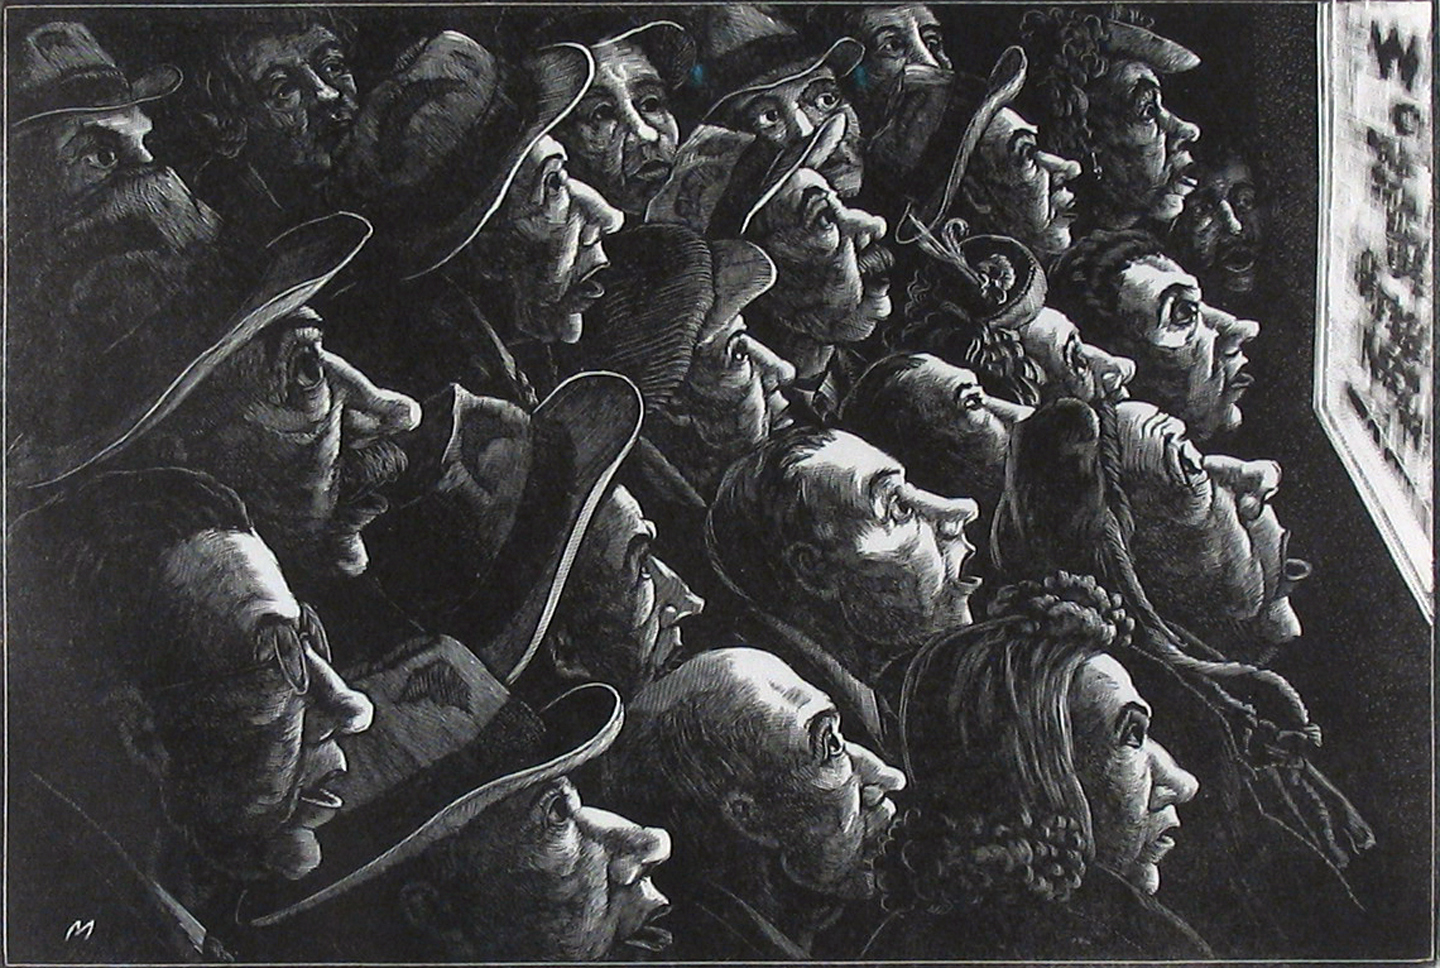
\includegraphics[width=17cm]{Pictures/Meissner_War_Bulletins.jpg}
\newpage
\section{Production Support - SUP1}
\label{sec-10}
\subsection{Support Databases}
\label{sec-10-1}

\scriptsize

\begin{center}
\begin{tabular}{llll}
\hline
 \textbf{USERNAME}  &  \textbf{PASSWORD}  &  \textbf{DB\_INSTANCE}  &  \textbf{Description}   \\
\hline
 PRDAFC             &  PRDAFC             &  SUPAF                  &  Reference Tables       \\
 PRDCUSTC           &  PRDCUSTC           &  SUPCUST                &  Customer               \\
 PRDRPLC            &  PRDRPLC            &  SUPRPL                 &  Replenishment Manager  \\
 PRDUSG1C           &  PRDUSG1C           &  SUPUSG1                &  Usage                  \\
 PRDUSG2C           &  PRDUSG2C           &  SUPUSG2                &  Usage                  \\
 PRDUSG3C           &  PRDUSG3C           &  SUPUSG3                &  Usage                  \\
 PRDUSG4C           &  PRDUSG4C           &  SUPUSG4                &  Usage                  \\
 PRDSELC            &  PRDSELC            &  SUPAPRM                &  APRM                   \\
\hline
\end{tabular}
\end{center}


\normalsize
\subsection{Support Server}
\label{sec-10-2}

   Accessed from Putty in \textbf{TOPS} Production Support Applications.
   Should be able to login on with LAN ID and password (which is same as your LAN ID).

\begin{center}
\begin{tabular}{l}
\hline
 \textbf{SERVER NAME}  \\
\hline
 Ksr01omsap.uscc.com   \\
 ksr01bmrim.uscc.com   \\
 ksr01csmap.uscc.com   \\
 ksr01batch.uscc.com   \\
 ksr01tiger.uscc.com   \\
 ksr01aprma.uscc.com   \\
 ksr01mcsap.uscc.com   \\
 ksr01ebiap.uscc.com   \\
 msr01esadm.uscc.com   \\
 msr01esb01.uscc.com   \\
 msr01esb02.uscc.com   \\
 msr01wladm.uscc.com   \\
 msr01wls01.uscc.com   \\
 msr01wls02.uscc.com   \\
 msr01web01.uscc.com   \\
 msr01web02.uscc.com   \\
\hline
\end{tabular}
\end{center}
\subsection{Development Servers}
\label{sec-10-3}

\footnotesize

\begin{center}
\begin{tabular}{lrlll}
\hline
 \textbf{Environment}  &   \textbf{IP}  &  \textbf{Hostname}  &  \textbf{UserID}  &  \textbf{Password}  \\
\hline
 Development           &   10.106.10.9  &  mdr01bld01         &  md1dbal1         &  \emph{password}    \\
 Testing               &   10.106.10.9  &  mdr01bld01         &  d\_medap         &  Henry*123          \\
 CallDump              &  10.176.179.3  &  kpr01scdap         &  calldmp          &  Henry*128          \\
\hline
\end{tabular}
\end{center}



\newpage
\section{Accounts Receivable}
\label{sec-11}

  Handles Finance, Payments and credits as well Collections. 
\subsection{AR Basics}
\label{sec-11-1}

\begin{itemize}
\item \textbf{Root Directory} - \$ABP\_AR\_ROOT on kpr01batch
\item \textbf{Collection Interface} - /pkgbl01/inf/aimsys/prdwrk1/var/usc/projs/cl/interfaces
\end{itemize}
\subsection{AR Jobs}
\label{sec-11-2}
\subsubsection{AR1JRNLEXT}
\label{sec-11-2-1}

    The Journal Extract process extracts to an output file all financial activities that occurred since the last run of this process.
\begin{itemize}
\item \textbf{LOG FILE} - AR1JRNLEXT.<SYS\_DATE>.log
\item \textbf{Output File} -
\item \textbf{Script Name} - ar1\_JrnlExtract\_Sh
\end{itemize}
\subsection{End of Month}
\label{sec-11-3}
\subsubsection{Email List for Revenue Accounting}
\label{sec-11-3-1}

\begin{verbatim}
        Tabano-lucero Glayn <Glayn.Tabano-lucero@uscellular.com>; 
        Rizwan, Muhammad <Muhammad.Rizwan@uscellular.com>; 
        Vann, John <John.Vann@uscellular.com>;
        Revenue Accounting <RevenueAccounting@uscellular.com>
\end{verbatim}
\subsubsection{Revenue Not confirmed for cycles 24,26 and 28}
\label{sec-11-3-2}

\begin{verbatim}
        select sum(amount),bcc.cycle_year,bcc.cycle_instance,bcc.cycle_code
         from bl1_inv_charge_rel bicr 
          inner join bl1_cycle_control bcc on bicr.cycle_seq_no=bcc.cycle_seq_no 
          inner join bl1_cyc_payer_pop bcpp on bcpp.period_key=bicr.period_key 
          and bcpp.customer_key=bicr.customer_key and bcpp.ba_no=bicr.ba_no
        where bcpp.status<>'CN' and bicr.period_key=20 and bcc.cycle_year=2015 
         and bcc.cycle_instance=8 and bcc.cycle_code in (24,26,28)
         group by bcc.cycle_year,bcc.cycle_instance,bcc.cycle_code
         order by bcc.cycle_year,bcc.cycle_instance,bcc.cycle_code;
\end{verbatim}
\subsubsection{Null GeoCodes}
\label{sec-11-3-3}

\begin{verbatim}
        select s_customer_id, s_fa_id, contact_id, cust.*, fa_rl.*, fa.*,con.*
         from sa.table_customer cust
          inner join sa.table_con_fin_accnt_role fa_rl 
                on fa_rl.fa_role2customer = cust.objid
          inner join sa.table_fin_accnt fa on fa_rl.fin_accnt_role2fin_accnt=fa.objid
          inner join sa.table_contact con on fa_rl.con_accnt_role2contact=con.objid
         where s_fa_id='851316127';
\end{verbatim}
\begin{itemize}

\item Query for the EOM
\label{sec-11-3-3-1}%
\begin{verbatim}
 select  distinct account_id,L9_GEO_CODE from ar1_account where account_id 
 in (select account_id from prdcustc.geo_code_09012014 where GEO_CODE in ('0','00'))
\end{verbatim}
\end{itemize} % ends low level
\subsection{Payment File}
\label{sec-11-4}

   Once in a while payment files break due to either bad sequence numbers or format issues. For the most part you should tell Amdocs to put the file in CN status and have \textbf{Payment Control} to resend.
   If the file is also out of sequence have payment control send it with a new sequence number. If the whole file fails, not just records, then have Payment Control send a new file with a new sequence number.
\begin{verbatim}
 PaymentControl-ImportPaymentFiles@uscellular.com>
\end{verbatim}
\subsection{AR Reports}
\label{sec-11-5}

\begin{itemize}
\item \textbf{LockBox}
\begin{itemize}
\item \emph{File Location} : \$ABP\_AR\_ROOT/interfaces/input/lockbox/MELL\_PYM.*.csv
\end{itemize}
\item \textbf{AGTCASH}
\begin{itemize}
\item \emph{File Location} : \$ABP\_AR\_ROOT/interfaces/input/lockbox/ACP\_PYM*.csv
\end{itemize}
\item \textbf{IMPCOL}
\begin{itemize}
\item \emph{File Location} : \$ABP\_AR\_ROOT/interfaces/input/lockbox/IMPCOL.PAY*.csv
\end{itemize}
\item \textbf{IMPEFT}
\begin{itemize}
\item \emph{File Location} : \$ABP\_AR\_ROOT/interfaces/input/lockbox/IMPEFT.PAY.*csv
\end{itemize}
\item \textbf{IMPPAY}
\begin{itemize}
\item \emph{File Location} : \$ABP\_AR\_ROOT/interfaces/input/lockbox/IMPPAY.PAY.*.csv
\end{itemize}
\item \textbf{Autopay Reports} \\ Both of these reports are derived after the above files have been processed.
\begin{itemize}
\item \textbf{Autopay\_PostPaid}
\begin{itemize}
\item Run both the expected and actual \textbf{SQL}
\end{itemize}
\item \textbf{Autopay\_PrePaid}
\begin{itemize}
\item Run prepaid expected \textbf{SQL}
\end{itemize}
\end{itemize}
\item \textbf{ACH extract file} \\Check to see if the output report and \textbf{SQL} match.
\begin{itemize}
\item \emph{File Location} : \$ABP\_AR\_ROOT/interfaces/output/ACH.ar.DD\_OUT*\\
\end{itemize}
\end{itemize}
\subsection{AR Tables}
\label{sec-11-6}
\subsubsection{AR1\_ACCOUNT}
\label{sec-11-6-1}

\scriptsize

\begin{center}
\begin{tabular}{lll}
\hline
 \textbf{Column Name}             &  \textbf{Data Type}  &  \textbf{Description}  \\
\hline
 \textbf{ACCOUNT\_ID}             &  NUMBER (12)         &  The Financial ID      \\
 ACCOUNT\_STATUS                  &  VARCHAR2 (4 Byte)   &                        \\
 ACCOUNT\_TIMESTAMP               &  NUMBER (19)         &                        \\
 ACCT\_BAL\_POLICY                &  CHAR (1 Byte)       &                        \\
 APPLICATION\_ID                  &  CHAR (6 Byte)       &                        \\
 \textbf{AR\_ACCOUNT\_SUB\_TYPE}  &  CHAR (4 Byte)       &                        \\
 \textbf{AR\_ACCOUNT\_TYPE}       &  CHAR (1 Byte)       &                        \\
 \textbf{AR\_BALANCE}             &  NUMBER (18,2)       &                        \\
 AR\_EXCEPTION\_ACC\_IND          &  CHAR (1 Byte)       &                        \\
 BALANCE\_UPD\_DATE               &  DATE                &                        \\
 BE                               &  NUMBER (9)          &                        \\
 CANDIDATE\_FILE\_EXTRACT\_DATE   &  DATE                &                        \\
 CM\_ACCOUNT\_NUMBER              &  VARCHAR2 (12 Byte)  &                        \\
 COLL\_IND\_UPD\_DATE             &  DATE                &                        \\
 COLLECTION\_INDICATOR            &  CHAR (1 Byte)       &                        \\
 CURRENCY                         &  CHAR (3 Byte)       &                        \\
 \textbf{CUSTOMER\_NO}            &  NUMBER (10)         &                        \\
 DEPOSIT\_BALANCE                 &  NUMBER (18,2)       &                        \\
 DISPUTE\_BALANCE                 &  NUMBER (18,2)       &                        \\
 DL\_SERVICE\_CODE                &  CHAR (5 Byte)       &                        \\
 DL\_UPDATE\_STAMP                &  NUMBER (4)          &                        \\
 DOCUMENT\_TYPE                   &  CHAR (6 Byte)       &                        \\
 L3\_AGREEMENT\_ID                &  NUMBER (9)          &                        \\
 L3\_BOD\_BALANCE                 &  NUMBER (18,2)       &                        \\
 L3\_CREDIT\_LIMIT\_IND           &  CHAR (1 Byte)       &                        \\
 L3\_NEW\_INVOICE\_IND            &  CHAR (1 Byte)       &                        \\
 L3\_SEND\_BALANCE                &  NUMBER (18,2)       &                        \\
 \textbf{L9\_GEO\_CODE}           &  VARCHAR2 (10 Byte)  &                        \\
 LAST\_ACTIVITY\_STATUS\_DATE     &  DATE                &                        \\
 LPC\_WAVING\_IND                 &  CHAR (1 Byte)       &                        \\
 OPERATOR\_ID                     &  NUMBER (9)          &                        \\
 PARTITION\_ID                    &  NUMBER (5)          &                        \\
 PENDING\_CREDIT\_BALANCE         &  NUMBER (18,2)       &                        \\
 SYS\_CREATION\_DATE              &  DATE                &                        \\
 SYS\_UPDATE\_DATE                &  DATE                &                        \\
 UNAPPLIED\_AMOUNT                &  NUMBER (18,2)       &                        \\
 WRITE\_OFF\_STATUS               &  CHAR (1 Byte)       &                        \\
\hline
\end{tabular}
\end{center}


\normalsize
\subsubsection{AR1\_INVOICE}
\label{sec-11-6-2}

\scriptsize
\begin{longtable}{lll}

\hline
 \textbf{Column Name}           &  \textbf{Data Type}   &  \textbf{Description} \\
\hline
\endhead
\hline\multicolumn{3}{r}{Continued on next page}\
\endfoot
\endlastfoot
 \textbf{ACCOUNT\_ID}           &  NUMBER (12)          &                        \\
 APPLICATION\_ID                &  CHAR (6 Byte)        &                        \\
 AR\_INVOICE\_NUMBER            &  VARCHAR2 (60 Byte)   &                        \\
 BILL\_SEQ\_NO                  &  NUMBER (12)          &                        \\
 BILLING\_ARRANGEMENT\_ID       &  NUMBER (12)          &                        \\
 BILLING\_INVOICE\_NUMBER       &  VARCHAR2 (180 Byte)  &                        \\
 CREDIT\_AMOUNT                 &  NUMBER (18,2)        &                        \\
 CREDIT\_NET\_AMOUNT            &  NUMBER (18,2)        &                        \\
 CREDIT\_TAX\_AMOUNT            &  NUMBER (18,2)        &                        \\
 \textbf{CYCLE\_CODE}           &  NUMBER (4)           &                        \\
 \textbf{CYCLE\_MONTH}          &  NUMBER (2)           &                        \\
 CYCLE\_YEAR                    &  NUMBER (4)           &                        \\
 DISCOUNT\_AMOUNT               &  NUMBER (18,2)        &                        \\
 DISCOUNT\_NET\_AMT             &  NUMBER (18,2)        &                        \\
 DISCOUNT\_TAX\_AMT             &  NUMBER (18,2)        &                        \\
 DL\_SERVICE\_CODE              &  CHAR (5 Byte)        &                        \\
 DL\_UPDATE\_STAMP              &  NUMBER (4)           &                        \\
 FINALISE\_DATE                 &  DATE                 &                        \\
 FINALISE\_TRANS\_ID            &  NUMBER (12)          &                        \\
 INVOICE\_AMOUNT                &  NUMBER (18,2)        &                        \\
 INVOICE\_BALANCE               &  NUMBER (18,2)        &                        \\
 INVOICE\_CREATION\_DATE        &  DATE                 &                        \\
 INVOICE\_ID                    &  NUMBER (12)          &                        \\
 INVOICE\_STATUS                &  VARCHAR2 (6 Byte)    &                        \\
 INVOICE\_STATUS\_CHANGE\_DATE  &  DATE                 &                        \\
 INVOICE\_TYPE                  &  VARCHAR2 (6 Byte)    &                        \\
 L3\_CRD\_EXTRACT\_IND          &  CHAR (1 Byte)        &                        \\
 OPERATOR\_ID                   &  NUMBER (9)           &                        \\
 PARTITION\_ID                  &  NUMBER (5)           &                        \\
 PERIOD\_KEY                    &  NUMBER (5)           &                        \\
 REVERSAL\_DATE                 &  DATE                 &                        \\
 REVERSAL\_TRANS\_ID            &  NUMBER (12)          &                        \\
 SUB\_BILL\_SEQ\_NO             &  NUMBER (12)          &                        \\
 SYS\_CREATION\_DATE            &  DATE                 &                        \\
 SYS\_UPDATE\_DATE              &  DATE                 &                        \\
 TAX\_AMOUNT                    &  NUMBER (18,2)        &                        \\
 TRANSACTION\_ID                &  NUMBER (12)          &                        \\
\hline
\end{longtable}

\normalsize
\subsubsection{AR1\_CHARGE\_CODE}
\label{sec-11-6-3}
\subsubsection{AR1\_CHARGE\_GROUP}
\label{sec-11-6-4}
\subsubsection{AR1\_CUSTOMER\_CREDIT}
\label{sec-11-6-5}

\scriptsize
\begin{longtable}{lll}

\hline
 \textbf{Column Name}          &  \textbf{Data Type}  &  \textbf{Description} \\
\hline
\endhead
\hline\multicolumn{3}{r}{Continued on next page}\
\endfoot
\endlastfoot
 ACCOUNT\_ID                   &  NUMBER (12)         &                        \\
 AMOUNT                        &  NUMBER (18,2)       &                        \\
 APPLICATION\_ID               &  CHAR (6 Byte)       &                        \\
 BALANCE\_IMPACT\_CODE         &  CHAR (1 Byte)       &                        \\
 BE                            &  NUMBER (9)          &                        \\
 BILL\_SEQ\_NO                 &  NUMBER (12)         &                        \\
 BILLING\_ARRANGEMENT\_ID      &  NUMBER (12)         &                        \\
 BILLING\_CHARGE\_SEQ\_NO      &  NUMBER (12)         &                        \\
 CHARGE\_CODE                  &  VARCHAR2 (25 Byte)  &                        \\
 CHG\_REVENUE\_CODE            &  CHAR (6 Byte)       &                        \\
 CR\_ATTRIB\_NAME              &  VARCHAR2 (30 Byte)  &                        \\
 CREDIT\_DATE                  &  DATE                &                        \\
 CREDIT\_ID                    &  NUMBER (12)         &                        \\
 CREDIT\_LEVEL\_CODE           &  CHAR (3 Byte)       &                        \\
 CREDIT\_REASON                &  VARCHAR2 (10 Byte)  &                        \\
 DL\_SERVICE\_CODE             &  CHAR (5 Byte)       &                        \\
 DL\_UPDATE\_STAMP             &  NUMBER (4)          &                        \\
 FINALISE\_DATE                &  DATE                &                        \\
 FINALISE\_TRANS\_ID           &  NUMBER (12)         &                        \\
 INVOICE\_ID                   &  NUMBER (12)         &                        \\
 INVOICE\_REVERSAL\_NUMBER     &  NUMBER (12)         &                        \\
 L9\_CANCEL\_IND               &  VARCHAR2 (2 Byte)   &                        \\
 L9\_DF\_ACTIVITY              &  VARCHAR2 (3 Byte)   &                        \\
 L9\_DF\_INDICATOR             &  VARCHAR2 (3 Byte)   &                        \\
 L9\_DF\_PERIOD                &  VARCHAR2 (3 Byte)   &                        \\
 L9\_EVENT\_ID                 &  NUMBER (18)         &                        \\
 L9\_IS\_DISCOUNT              &  VARCHAR2 (1 Byte)   &                        \\
 L9\_LINE\_COUNT               &  NUMBER (5)          &                        \\
 L9\_LOCATION                  &  VARCHAR2 (15 Byte)  &                        \\
 L9\_LT\_AMOUNT                &  NUMBER (18,2)       &                        \\
 L9\_ORIG\_CHARGE\_TYPE        &  VARCHAR2 (3 Byte)   &                        \\
 L9\_ORIG\_CHG\_SEQ\_NO        &  NUMBER (12)         &                        \\
 L9\_REV\_LOCATION             &  VARCHAR2 (15 Byte)  &                        \\
 L9\_REV\_SALES\_CHANNEL       &  VARCHAR2 (15 Byte)  &                        \\
 L9\_SALES\_CHANNEL            &  VARCHAR2 (15 Byte)  &                        \\
 L9\_ST\_AMOUNT                &  NUMBER (18,2)       &                        \\
 OPERATOR\_ID                  &  NUMBER (9)          &                        \\
 PARTITION\_ID                 &  NUMBER (5)          &                        \\
 PERIOD\_KEY                   &  NUMBER (5)          &                        \\
 RESTRICTED\_CHARGE\_ID        &  NUMBER (12)         &                        \\
 RESTRICTED\_INVOICE\_NUMBER   &  NUMBER (12)         &                        \\
 REVERSAL\_BILL\_SEQ\_NO       &  NUMBER (12)         &                        \\
 REVERSAL\_DATE                &  DATE                &                        \\
 REVERSAL\_REASON              &  VARCHAR2 (10 Byte)  &                        \\
 REVERSAL\_SUB\_BILL\_SEQ\_NO  &  NUMBER (12)         &                        \\
 REVERSAL\_TRANS\_ID           &  NUMBER (12)         &                        \\
 SUB\_BILL\_SEQ\_NO            &  NUMBER (12)         &                        \\
 SYS\_CREATION\_DATE           &  DATE                &                        \\
 SYS\_UPDATE\_DATE             &  DATE                &                        \\
 TAX\_AMOUNT                   &  NUMBER (18,2)       &                        \\
 TRANSACTION\_ID               &  NUMBER (12)         &                        \\
 WRITE\_OFF\_ID                &  NUMBER (12)         &                        \\
\hline
\end{longtable}

\normalsize
\subsubsection{AR1\_TAX\_ITEM}
\label{sec-11-6-6}
\subsubsection{AR1\_REFUND\_REQUEST}
\label{sec-11-6-7}

\scriptsize
\begin{longtable}{lll}

\hline
 \textbf{Column Name}           &  \textbf{Data Type}  &  \textbf{Description} \\
\hline
\endhead
\hline\multicolumn{3}{r}{Continued on next page}\
\endfoot
\endlastfoot
 ACCOUNT\_ID                    &  NUMBER (12)         &                        \\
 ACTIVITY\_DATE                 &  DATE                &                        \\
 AMOUNT                         &  NUMBER (18,2)       &                        \\
 APPLICATION\_ID                &  CHAR (6 Byte)       &                        \\
 APPLICATION\_METHOD            &  VARCHAR2 (5 Byte)   &                        \\
 CREDIT\_ID                     &  NUMBER (12)         &                        \\
 CRITERIA\_ID                   &  NUMBER (12)         &                        \\
 DEBIT\_ID                      &  NUMBER (12)         &                        \\
 DL\_SERVICE\_CODE              &  CHAR (5 Byte)       &                        \\
 DL\_UPDATE\_STAMP              &  NUMBER (4)          &                        \\
 EXTRACT\_TO\_AP\_DATE          &  DATE                &                        \\
 L9\_BUY\_BACK\_PREPAID         &  VARCHAR2 (2 Byte)   &                        \\
 L9\_CITY                       &  VARCHAR2 (35 Byte)  &                        \\
 L9\_CUSTOMER\_NAME             &  VARCHAR2 (50 Byte)  &                        \\
 L9\_LOCATION                   &  VARCHAR2 (15 Byte)  &                        \\
 L9\_MERCHANT\_REFERENCE\_CODE  &  NUMBER (8)          &                        \\
 L9\_POSTAL\_CODE               &  VARCHAR2 (10 Byte)  &                        \\
 L9\_REGION                     &  VARCHAR2 (3 Byte)   &                        \\
 L9\_REQUEST\_ID                &  VARCHAR2 (26 Byte)  &                        \\
 L9\_REV\_LOCATION              &  VARCHAR2 (15 Byte)  &                        \\
 L9\_REV\_SALES\_CHANNEL        &  VARCHAR2 (15 Byte)  &                        \\
 L9\_SALES\_CHANNEL             &  VARCHAR2 (15 Byte)  &                        \\
 L9\_STREET                     &  VARCHAR2 (35 Byte)  &                        \\
 MANUAL\_REFUND\_IND            &  CHAR (1 Byte)       &                        \\
 OPERATOR\_ID                   &  NUMBER (9)          &                        \\
 PARTITION\_ID                  &  NUMBER (5)          &                        \\
 REFUND\_ID                     &  NUMBER (12)         &                        \\
 REFUND\_METHOD                 &  VARCHAR2 (3 Byte)   &                        \\
 REFUND\_REASON                 &  VARCHAR2 (10 Byte)  &                        \\
 REFUND\_STATUS                 &  CHAR (1 Byte)       &                        \\
 REVERSAL\_CREDIT\_ID           &  NUMBER (12)         &                        \\
 REVERSAL\_DATE                 &  DATE                &                        \\
 REVERSAL\_REASON               &  VARCHAR2 (10 Byte)  &                        \\
 REVERSAL\_TRANS\_ID            &  NUMBER (12)         &                        \\
 SYS\_CREATION\_DATE            &  DATE                &                        \\
 SYS\_UPDATE\_DATE              &  DATE                &                        \\
 TRANSACTION\_ID                &  NUMBER (12)         &                        \\
\hline
\end{longtable}


\normalsize
\subsubsection{AR1\_DEPOSIT\_REQUEST}
\label{sec-11-6-8}

\scriptsize
\begin{longtable}{lll}

\hline
 \textbf{Column Name}   &  \textbf{Data Type}  &  \textbf{Description} \\
\hline
\endhead
\hline\multicolumn{3}{r}{Continued on next page}\
\endfoot
\endlastfoot
 ACCOUNT\_ID            &  NUMBER (12)         &                        \\
 APPLICATION\_ID        &  CHAR (6 Byte)       &                        \\
 CANCEL\_DATE           &  DATE                &                        \\
 CANCEL\_REASON         &  VARCHAR2 (6 Byte)   &                        \\
 CANCELLED\_AMOUNT      &  NUMBER (18,2)       &                        \\
 DEBIT\_ID              &  NUMBER (12)         &                        \\
 DEPOSIT\_DESIGNATION   &  VARCHAR2 (20 Byte)  &                        \\
 DEPOSIT\_ID            &  NUMBER (12)         &                        \\
 DL\_SERVICE\_CODE      &  CHAR (5 Byte)       &                        \\
 DL\_UPDATE\_STAMP      &  NUMBER (4)          &                        \\
 DUE\_DATE              &  DATE                &                        \\
 EXTERNAL\_DEPOSIT\_ID  &  VARCHAR2 (20 Byte)  &                        \\
 GROUP\_ID              &  VARCHAR2 (20 Byte)  &                        \\
 INTEREST\_AMOUNT       &  NUMBER (18,2)       &                        \\
 L9\_AP\_ID             &  VARCHAR2 (10 Byte)  &                        \\
 L9\_EXT\_CHG\_ID       &  NUMBER (12)         &                        \\
 L9\_LOCATION           &  VARCHAR2 (15 Byte)  &                        \\
 L9\_SALES\_CHANNEL     &  VARCHAR2 (15 Byte)  &                        \\
 OPERATOR\_ID           &  NUMBER (9)          &                        \\
 PAID\_DATE             &  DATE                &                        \\
 PARENT\_DEPOSIT\_ID    &  NUMBER (12)         &                        \\
 PARTITION\_ID          &  NUMBER (5)          &                        \\
 PYMT\_TRIGGERED        &  CHAR (1 Byte)       &                        \\
 RELEASE\_DATE          &  DATE                &                        \\
 RELEASE\_METHOD        &  VARCHAR2 (6 Byte)   &                        \\
 RELEASE\_REASON        &  VARCHAR2 (6 Byte)   &                        \\
 RELEASED\_AMOUNT       &  NUMBER (18,2)       &                        \\
 REQUEST\_AMOUNT        &  NUMBER (18,2)       &                        \\
 REQUEST\_DATE          &  DATE                &                        \\
 REQUEST\_REASON        &  VARCHAR2 (6 Byte)   &                        \\
 REVERSAL\_TRANS\_ID    &  NUMBER (12)         &                        \\
 SYS\_CREATION\_DATE    &  DATE                &                        \\
 SYS\_UPDATE\_DATE      &  DATE                &                        \\
 TRANSACTION\_ID        &  NUMBER (12)         &                        \\
\hline
\end{longtable}

\normalsize
\subsubsection{AR1\_PAYMENT}
\label{sec-11-6-9}

\scriptsize
\begin{longtable}{lll}

\hline
 \textbf{Column Name}         &  \textbf{Data Type}  &  \textbf{Description} \\
\hline
\endhead
\hline\multicolumn{3}{r}{Continued on next page}\
\endfoot
\endlastfoot
 ACCOUNT\_ID                  &  NUMBER (12)         &                        \\
 ACTIVITY\_DATE               &  DATE                &                        \\
 ACTIVITY\_INDICATOR          &  CHAR (5 Byte)       &                        \\
 AMOUNT                       &  NUMBER (18,2)       &                        \\
 APPLICATION\_ID              &  CHAR (6 Byte)       &                        \\
 BILL\_SEQ\_NO                &  NUMBER (12)         &                        \\
 CONVERSION\_RATE             &  NUMBER (11,9)       &                        \\
 CREDIT\_ID                   &  NUMBER (12)         &                        \\
 DL\_SERVICE\_CODE            &  CHAR (5 Byte)       &                        \\
 DL\_UPDATE\_STAMP            &  NUMBER (4)          &                        \\
 L9\_DEP\_REL                 &  CHAR (1 Byte)       &                        \\
 L9\_LOCATION                 &  VARCHAR2 (15 Byte)  &                        \\
 L9\_SALES\_CHANNEL           &  VARCHAR2 (15 Byte)  &                        \\
 OPERATOR\_ID                 &  NUMBER (9)          &                        \\
 ORIGINAL\_AMOUNT             &  NUMBER (18,2)       &                        \\
 ORIGINAL\_CONVERTED\_AMOUNT  &  NUMBER (18,2)       &                        \\
 PARTITION\_ID                &  NUMBER (5)          &                        \\
 PAYMENT\_ID                  &  NUMBER (12)         &                        \\
 PERIOD\_KEY                  &  NUMBER (5)          &                        \\
 PYMDT\_PARTITION\_ID         &  NUMBER (5)          &                        \\
 PYMDT\_PERIOD\_KEY           &  NUMBER (5)          &                        \\
 REVERSAL\_TRANS\_ID          &  NUMBER (12)         &                        \\
 SUB\_BILL\_SEQ\_NO           &  NUMBER (12)         &                        \\
 SYS\_CREATION\_DATE          &  DATE                &                        \\
 SYS\_UPDATE\_DATE            &  DATE                &                        \\
 TRANSACTION\_ID              &  NUMBER (12)         &                        \\
\hline
\end{longtable}



\normalsize
\subsubsection{AR1\_PAYMENT\_DETAILS}
\label{sec-11-6-10}

\scriptsize
\begin{longtable}{lll}

\hline
 \textbf{Column Name}           &  \textbf{Data Type}   &  \textbf{Description} \\
\hline
\endhead
\hline\multicolumn{3}{r}{Continued on next page}\
\endfoot
\endlastfoot
 ACCOUNT\_ID                    &  NUMBER (12)          &                        \\
 AMOUNT                         &  NUMBER (18,2)        &                        \\
 APPLICATION\_ID                &  CHAR (6 Byte)        &                        \\
 BANK\_ACCOUNT\_NUMBER          &  VARCHAR2 (255 Byte)  &                        \\
 BANK\_BRANCH\_NUMBER           &  VARCHAR2 (20 Byte)   &                        \\
 BANK\_CODE                     &  VARCHAR2 (20 Byte)   &                        \\
 BATCH\_LINE\_NUMBER            &  NUMBER (6)           &                        \\
 BATCH\_NUMBER                  &  NUMBER (5)           &                        \\
 BILLING\_ARRANGEMENT           &  NUMBER (12)          &                        \\
 BILLING\_INVOICE\_NUMBER       &  VARCHAR2 (180 Byte)  &                        \\
 CC\_AUTHORISATION\_CODE        &  VARCHAR2 (8 Byte)    &                        \\
 CC\_EXPIRY\_DATE               &  VARCHAR2 (6 Byte)    &                        \\
 CHECK\_DRAWER\_NAME            &  VARCHAR2 (30 Byte)   &                        \\
 CHECK\_NO                      &  VARCHAR2 (15 Byte)   &                        \\
 CONFIRMATION\_NO               &  VARCHAR2 (20 Byte)   &                        \\
 CREDIT\_CARD\_NUMBER           &  VARCHAR2 (255 Byte)  &                        \\
 CURRENCY                       &  CHAR (3 Byte)        &                        \\
 DEPOSIT\_DATE                  &  DATE                 &                        \\
 DEPOSIT\_DESIGNATION           &  VARCHAR2 (20 Byte)   &                        \\
 DIRECT\_DEBIT\_VOUCHER         &  NUMBER (12)          &                        \\
 DL\_SERVICE\_CODE              &  CHAR (5 Byte)        &                        \\
 DL\_UPDATE\_STAMP              &  NUMBER (4)           &                        \\
 FILE\_GENERATION\_DATE         &  DATE                 &                        \\
 FILE\_SEQ\_NO                  &  NUMBER (5)           &                        \\
 FILE\_SOURCE\_ID               &  VARCHAR2 (8 Byte)    &                        \\
 FILE\_SOURCE\_TYPE             &  VARCHAR2 (4 Byte)    &                        \\
 L9\_AUTHORIZATION\_CODE        &  VARCHAR2 (7 Byte)    &                        \\
 L9\_CTN                        &  NUMBER (10)          &                        \\
 L9\_EXT\_PYM\_ID               &  VARCHAR2 (32 Byte)   &                        \\
 L9\_LOCATION                   &  VARCHAR2 (15 Byte)   &                        \\
 L9\_MERCHANT\_ID               &  VARCHAR2 (30 Byte)   &                        \\
 L9\_MERCHANT\_REFERENCE\_CODE  &  NUMBER (8)           &                        \\
 L9\_ORIG\_ACCOUNT              &  NUMBER (12)          &                        \\
 L9\_ORIG\_CHECK\_AMT           &  NUMBER (18,2)        &                        \\
 L9\_ORIGINATOR                 &  VARCHAR2 (20 Byte)   &                        \\
 L9\_ORIGINATOR\_LOCATION       &  VARCHAR2 (20 Byte)   &                        \\
 L9\_PAYMENT\_RECURRANCE        &  CHAR (1 Byte)        &                        \\
 L9\_REQUEST\_ID                &  VARCHAR2 (26 Byte)   &                        \\
 L9\_SALES\_CHANNEL             &  VARCHAR2 (15 Byte)   &                        \\
 MEMO\_ID                       &  NUMBER (12)          &                        \\
 OPERATOR\_ID                   &  NUMBER (9)           &                        \\
 PARTITION\_ID                  &  NUMBER (5)           &                        \\
 PAYMENT\_ID                    &  NUMBER (12)          &                        \\
 PAYMENT\_METHOD                &  CHAR (3 Byte)        &                        \\
 PAYMENT\_SOURCE\_ID            &  VARCHAR2 (15 Byte)   &                        \\
 PAYMENT\_SOURCE\_TYPE          &  VARCHAR2 (3 Byte)    &                        \\
 PAYMENT\_SUB\_METHOD           &  VARCHAR2 (3 Byte)    &                        \\
 PAYMENT\_TYPE                  &  CHAR (1 Byte)        &                        \\
 PERIOD\_KEY                    &  NUMBER (5)           &                        \\
 RECALL\_NUMBER                 &  VARCHAR2 (15 Byte)   &                        \\
 REJECTION\_CODE                &  VARCHAR2 (4 Byte)    &                        \\
 REVERSAL\_REASON               &  VARCHAR2 (10 Byte)   &                        \\
 SUBSCRIBER\_NUMBER             &  VARCHAR2 (11 Byte)   &                        \\
 SYS\_CREATION\_DATE            &  DATE                 &                        \\
 SYS\_UPDATE\_DATE              &  DATE                 &                        \\
 TRANSACTION\_ID                &  NUMBER (12)          &                        \\
\hline
\end{longtable}

\normalsize
\subsubsection{AR1\_PAYMENT\_ACTIVITY}
\label{sec-11-6-11}

    Used in the \textbf{Paid and Prepaid} reports.
\scriptsize
\begin{longtable}{lll}

\hline
 \textbf{Column Name}     &  \textbf{Data Type}  &  \textbf{Description} \\
\hline
\endhead
\hline\multicolumn{3}{r}{Continued on next page}\
\endfoot
\endlastfoot
 ACCOUNT\_ID              &  NUMBER (12)         &                        \\
 ACTIVITY\_DATE           &  DATE                &                        \\
 ACTIVITY\_TYPE           &  CHAR (5 Byte)       &                        \\
 AMOUNT                   &  NUMBER (18,2)       &                        \\
 APPLICATION\_ID          &  CHAR (6 Byte)       &                        \\
 BILL\_SEQ\_NO            &  NUMBER (12)         &                        \\
 CREDIT\_ID               &  NUMBER (12)         &                        \\
 DL\_SERVICE\_CODE        &  CHAR (5 Byte)       &                        \\
 DL\_UPDATE\_STAMP        &  NUMBER (4)          &                        \\
 FUNDS\_TRANSFER\_IND     &  VARCHAR2 (6 Byte)   &                        \\
 FUNDS\_TRANSFER\_REASON  &  VARCHAR2 (10 Byte)  &                        \\
 L9\_BATCH\_LINE\_NUMBER  &  NUMBER (7)          &                        \\
 L9\_BATCH\_NUMBER        &  NUMBER (6)          &                        \\
 L9\_FILE\_NAME           &  VARCHAR2 (50 Byte)  &                        \\
 L9\_LOCATION             &  VARCHAR2 (15 Byte)  &                        \\
 L9\_SALES\_CHANNEL       &  VARCHAR2 (15 Byte)  &                        \\
 MEMO\_ID                 &  NUMBER (12)         &                        \\
 OPERATOR\_ID             &  NUMBER (9)          &                        \\
 PARENT\_CREDIT           &  NUMBER (12)         &                        \\
 PARTITION\_ID            &  NUMBER (5)          &                        \\
 PAYMENT\_ACTIVITY\_ID    &  NUMBER (12)         &                        \\
 PAYMENT\_PERIOD\_KEY     &  NUMBER (5)          &                        \\
 PERIOD\_KEY              &  NUMBER (5)          &                        \\
 REASON\_CODE             &  VARCHAR2 (10 Byte)  &                        \\
 REVERSAL\_DATE           &  DATE                &                        \\
 REVERSAL\_REASON         &  VARCHAR2 (10 Byte)  &                        \\
 REVERSAL\_TRANS\_ID      &  NUMBER (12)         &                        \\
 SUB\_BILL\_SEQ\_NO       &  NUMBER (12)         &                        \\
 SYS\_CREATION\_DATE      &  DATE                &                        \\
 SYS\_UPDATE\_DATE        &  DATE                &                        \\
 TRANSACTION\_ID          &  NUMBER (12)         &                        \\
 TRANSFER\_ACCOUNT        &  NUMBER (12)         &                        \\
\hline
\end{longtable}

\normalsize
\subsection{Credit Cards}
\label{sec-11-7}
\subsubsection{AR9\_CC\_AUTH\_LOG}
\label{sec-11-7-1}

    Credit card transactions from the \textbf{TOPS} side.
\subsubsection{CTLOG}
\label{sec-11-7-2}

    Database from the microtelecom side.
\subsection{GL Tables}
\label{sec-11-8}
\subsubsection{ar1\_gl\_detailed\_data\_info\_v}
\label{sec-11-8-1}
\subsubsection{ar1\_gl\_data\_info\_v}
\label{sec-11-8-2}
\subsubsection{ar1\_transaction\_log}
\label{sec-11-8-3}
\subsubsection{ar1-JGL-control}
\label{sec-11-8-4}
\subsection{Operational SQL}
\label{sec-11-9}

   All of these scripts would be good monitor scripts.
\begin{itemize}
\item Checks to see if all payment files have been processed.(\textbf{PRDAF})
\end{itemize}
\begin{verbatim}
 select  identifier, nxt_pgm_name, file_status, file_format, file_name, file_path,  a.* 
  from ac1_control a
  where nxt_pgm_name like 'AR1PYM%'
  --and file_name like '%_181_%'
  and file_status <> 'CO'
  order by sys_creation_date desc 
\end{verbatim}
\begin{itemize}
\item Gateway Listener (\textbf{PRDCUST})
\end{itemize}
\begin{verbatim}
 select * from ar3_gwls_file_status 
  where sys_creation_date > (sysdate -6)
  and file_process_state <> 'CO' 
  order by sys_creation_date desc
\end{verbatim}
\begin{itemize}
\item More General stuff (\textbf{PRDCUST})
\end{itemize}
\begin{verbatim}
 select  trunc(sys_creation_date), period_key, record_type , 
  decode(record_type, 'PNR' , 'DONE' , 'LNR' , 'IN PROGRESS', 'NNR', 'PENDING') status  
  ,count(*) from ar1_jgl_control 
 where financial_activity_type is null  
  and sys_creation_date > to_date('20150826','yyyymmdd')
  group by  trunc(sys_creation_date), period_key , record_type
  order by 1, 2, 3  
\end{verbatim}
\begin{itemize}
\item Query for Batch Payments
\end{itemize}
\begin{verbatim}
 select count(1),sum(amount),trunc(sys_creation_date),deposit_date,payment_source_id,
  file_seq_no from ar1_payment_details
 where payment_source_id in ( 'LOCKBOX', 'AGTCASH', 'IMPCOL', 'IMPEFT', 'IMPPAY'
  ,'CERLBX') and sys_creation_date like '05-AUG-15%'
  and payment_type='P'
 group by  trunc(sys_creation_date), deposit_date, payment_source_id, file_seq_no
 order by  trunc(sys_creation_date), deposit_date, payment_source_id, file_seq_no
\end{verbatim}
\section{CallDump}
\label{sec-12}
\subsection{Data Directories}
\label{sec-12-1}

\begin{itemize}
\item \textbf{/m04/switchb/ecs} - \textbf{(aaa1)} 3G or lower data usage guide by \textbf{#19}.
\item \textbf{/m06/switch/MMS} - Picture Messaging
\item \textbf{/m06/switch/MMSText} - Picture Messaging Text only.
\item \textbf{/m06/switch/sms\_nsn} - SMS Motorola
\item \textbf{/m06/switchb/sms\_alu} - SMS ALU
\item \textbf{/m04/switch/lte} - \textbf{(aaa3)} P-Gateway 4G usage
\item \textbf{/m04/switchb/valista} - Premium SMS
\item \textbf{/m05/switch/brew} - Brew and Brew data \textbf{(aaa2)}
\item \textbf{/m01/switchb/tas} - Volte
\end{itemize}
\newpage
\section{Telephone Numbers}
\label{sec-13}

\huge
\begin{longtable}{ll}

\hline
 \textbf{Name}    &  \textbf{Cell} \\
\hline
\endhead
\hline\multicolumn{2}{r}{Continued on next page}\
\endfoot
\endlastfoot
 Vanessa          &   608-441-7106  \\
 Alex             &   608-219-7641  \\
 Dexter           &   608-219-5832  \\
 Dr. Smith        &   608-263-7500  \\
 Chuck            &   630-710-5201  \\
 Cindy            &   608-516-4539  \\
 Deb              &   312-810-1111  \\
 DC Operations    &   865-777-8771  \\
 Escalate Ticket  &   217-766-1979  \\
 Steve            &   608-222-5222  \\
 Ron W            &   651-734-8230  \\
 Paul Volpe       &   773-216-5606  \\
 Aunt Patty       &   256-772-7512  \\
 Help Desk:       &   608-828-5889  \\
 Soly             &   630-285-8386  \\
 Traci            &   630-285-8447  \\
\hline
\end{longtable}

\normalsize

\end{document}
